%%%%%%%%%%%%%%%%%%%%%%%%%%%%%%%%%%%%%%%%%%%%%%%%%%%%%%%%%%%%%%%%%
%                                                               %
%        NamedGraphs       encodage : utf8                      %
%                                                               %
%%%%%%%%%%%%%%%%%%%%%%%%%%%%%%%%%%%%%%%%%%%%%%%%%%%%%%%%%%%%%%%%%
%                                                               %
%           Créé par Alain Matthes le 14/03/2007                %
%  Copyright (c) 2007 __Collège Sévigné__ All rights reserved.  %
%        version : 1.0                                          %
%%%%%%%%%%%%%%%%%%%%%%%%%%%%%%%%%%%%%%%%%%%%%%%%%%%%%%%%%%%%%%%%%
% This file may be distributed and/or modified
%
% 1. under the LaTeX Project Public License , either version 1.3
% of this license or (at your option) any later version and/or
% 2. under the GNU Public License.
% See http://www.latex-project.org/lppl.txt for details.    
% graphs from graph theory

\documentclass[DIV         = 12,
               fontsize    = 10,
               headinclude = false,
               index       = totoc,
               footinclude = false,
               twoside,
               headings    = small
               ]{tkz-doc}  
%\usepackage{svn-multi} 
\usepackage{tkz-berge} 

\usepackage[pdftex,
            unicode,
            colorlinks    = true,
            pdfpagelabels, 
            urlcolor      = blue,
            filecolor     = pdffilecolor,
            linkcolor     = blue,
            breaklinks    = false,
            hyperfootnotes= false,
            bookmarks     = false,
            bookmarksopen = false, 
            linktocpage   = true,
            pdfsubject    ={Graph Theory},
            pdfauthor     ={Alain Matthes},
            pdftitle      ={NamedGraphs},
            pdfkeywords   ={graph,berge},
            pdfcreator    ={pdfeTeX}
            ]{hyperref}    
\usepackage{url}
\def\UrlFont{\small\ttfamily}
\usepackage[protrusion = true,
            expansion,
            final,
            verbose    = false
            ]{microtype}

\DisableLigatures{encoding = T1, family = tt*} 

\usepackage[parfill]{parskip}
\gdef\nameofpack{NamedGraphs}
\gdef\versionofpack{v 1.00 c}
\gdef\dateofpack{2011/05/26}
\gdef\nameofdoc{NamedGraphs}
\gdef\dateofdoc{2011/05/26}
\gdef\authorofpack{Alain Matthes}
\gdef\adressofauthor{}
\gdef\namecollection{AlterMundus}
\gdef\urlauthor{http://altermundus.fr}
\gdef\urlauthorcom{http://altermundus.com}
\title{The package : NamedGraphs}
\author{Alain Matthes}
   
\usepackage{shortvrb,fancyvrb}
\usepackage[saved]{tkzexample}
\def\tkzFileSavedPrefix{tkzNamed}
\makeatletter
\renewcommand*\l@subsubsection{\bprot@dottedtocline{3}{3.8em}{4.2em}}
\makeatother
\AtBeginDocument{\MakeShortVerb{\|}}

\pdfcompresslevel=9
\pdfinfo{
    /Title (NamedGraphs.pdf)
    /Creator (TeX)
    /Producer (pdfeTeX)
    /Author (Alain Matthes)
    /CreationDate (26 mai 2011)
    /Subject (Named Graphs)
    /Keywords (pdfeTeX, graph, cyclic, berge, tikz, pdflatex) }
    
\usepackage[english]{babel}
\usepackage[autolanguage]{numprint}  
%<---------------------------------------------------------------------------> 
\begin{document}
\parindent=0pt   
\title{\nameofpack}
\date{\today}

\clearpage
\thispagestyle{empty}
\maketitle

\clearpage
\tkzSetUpColors[background=fondpaille,text=Maroon]   
\colorlet{textcodecolor}{Maroon} 
\pagecolor{fondpaille} 
\color{Maroon}   
\colorlet{graphicbackground}{fondpaille}
\colorlet{codebackground}{Peach!30}
\colorlet{codeonlybackground}{Peach!30}   


\nameoffile{\nameofpack} 

\defoffile{\textbf{NamedGraphs.pdf} is not a beginner or advanced tutorial, not a study of graphs, it's only a gallery of undirected graphs made with  the package \textcolor{red}{tkz-berge.sty v 1.00 c}.  Some of  graphs  have names, sometimes inspired by the graph's topology, and sometimes after their discoverer. \textbf{NamedGraphs.pdf} presents some of them. A lot of references can be found here  \url{http://mathworld.wolfram.com}
}

\presentation

\vspace{1cm}

\tkzHand Firstly, I would like to thank \textbf{Till Tantau} for the  beautiful LATEX package, namely TikZ.

\tkzHand I am grateful to  \textbf{Michel Bovani} for providing the \tkzname{fourier} font.

\tkzHand I received much valuable advice and guidance on Graph Theory from \textbf{Rafael Villarroel}\\ \url{http://graphtheoryinlatex.blogspot.com/}.

\tkzHand The names of  graphs can be found here  \href{http://mathworld.wolfram.com/topics/SimpleGraphs.html}%
           {\textcolor{blue}{MathWorld}} by \href{http://en.wikipedia.org/wiki/Eric_W._Weisstein}%
           {\textcolor{blue}{E.Weisstein}}


\clearpage
\tableofcontents
 
\clearpage\newpage 
   
\setlength{\parskip}{1ex plus 0.5ex minus 0.2ex}
\tkzSetUpColors[background=fondpaille,text=Maroon]       
%!TEX root = /Users/ego/Boulot/TKZ/tkz-berge/NamedGraphs/doc/NamedGraphs-main.tex
\newpage\section{Andrasfai graph}
%<–––––––––––––––––––––––––––––––––––––––––––––––––––––––––––––––––––––––––>
%                               Andrasfai
%<–––––––––––––––––––––––––––––––––––––––––––––––––––––––––––––––––––––––––>
\begin{NewMacroBox}{grAndrasfai}{\oarg{options}\var{$k$}}

\medskip
From MathWord : \url{http://mathworld.wolfram.com/AndrasfaiGraph.html} 

\emph{The k-Andrásfai graph is a circulant graph on $3k-1$ nodes whose indices are given by the integers 1,\dots,$3k-1$  that are congruent to 1 (mod 3).
\href{http://mathworld.wolfram.com/topics/GraphTheory.html}%
           {\textcolor{blue}{MathWorld}} by \href{http://en.wikipedia.org/wiki/Eric_W._Weisstein}%
           {\textcolor{blue}{E.Weisstein}}
}

\medskip
\end{NewMacroBox}

\bigskip

\subsection{\tkzname{Andrásfai graph : k=7, order 20}}

\bigskip
\begin{center}
\begin{tkzexample}[vbox]
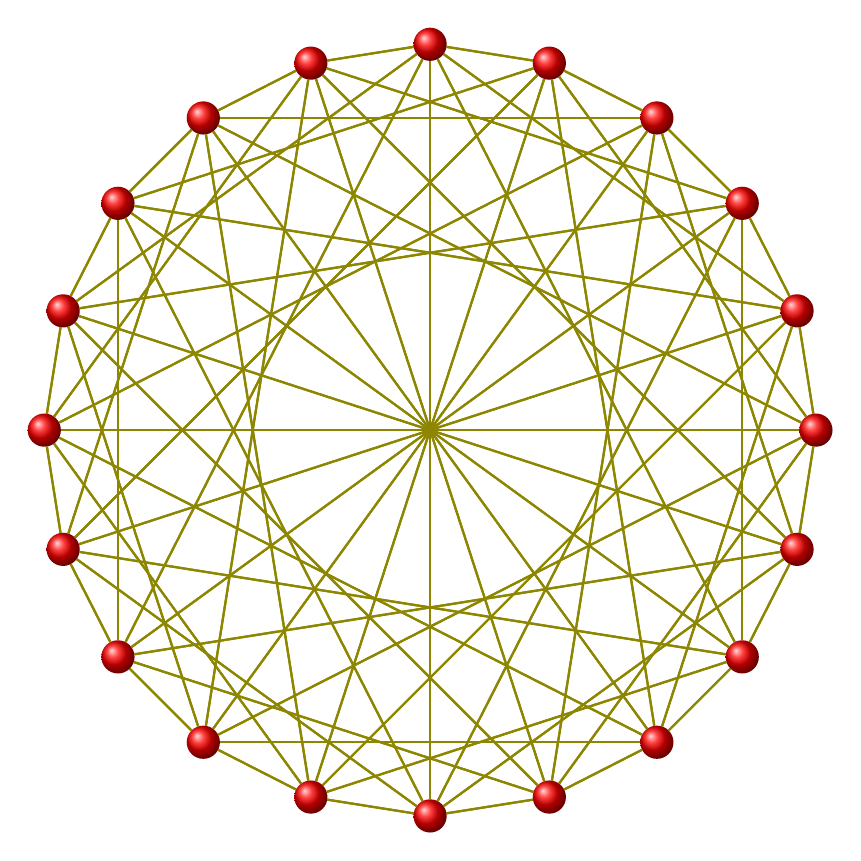
\begin{tikzpicture}[scale=.7]
  \GraphInit[vstyle=Art]
  \SetGraphArtColor{red}{olive}
  \grAndrasfai[RA=7]{7}
 \end{tikzpicture}
\end{tkzexample} 
\end{center}

\vfill\newpage
\subsection{\tkzname{Andrásfai graph :  k=8, order 23}}

\bigskip\begin{center}
\begin{tkzexample}[vbox]
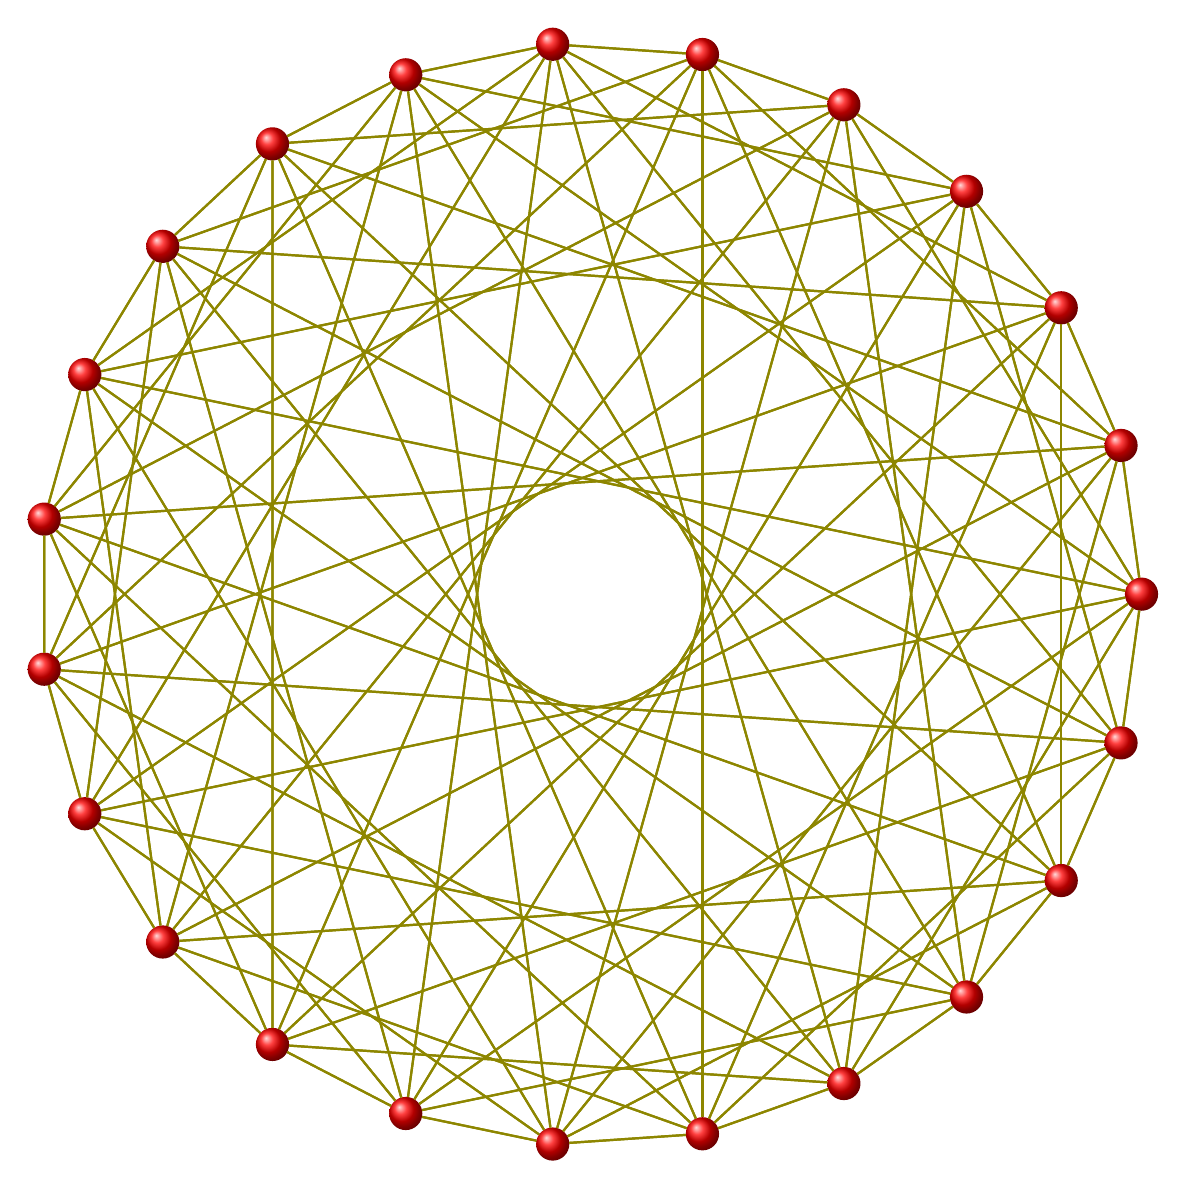
\begin{tikzpicture}
  \GraphInit[vstyle=Art]
  \SetGraphArtColor{red}{olive}
  \grAndrasfai[RA=7]{8}
  \end{tikzpicture}
\end{tkzexample} 
\end{center}


\vfill\newpage
\subsection{\tkzname{Andrásfai graph :  k=9, order 26}}

\bigskip\begin{center}
\begin{tkzexample}[vbox]
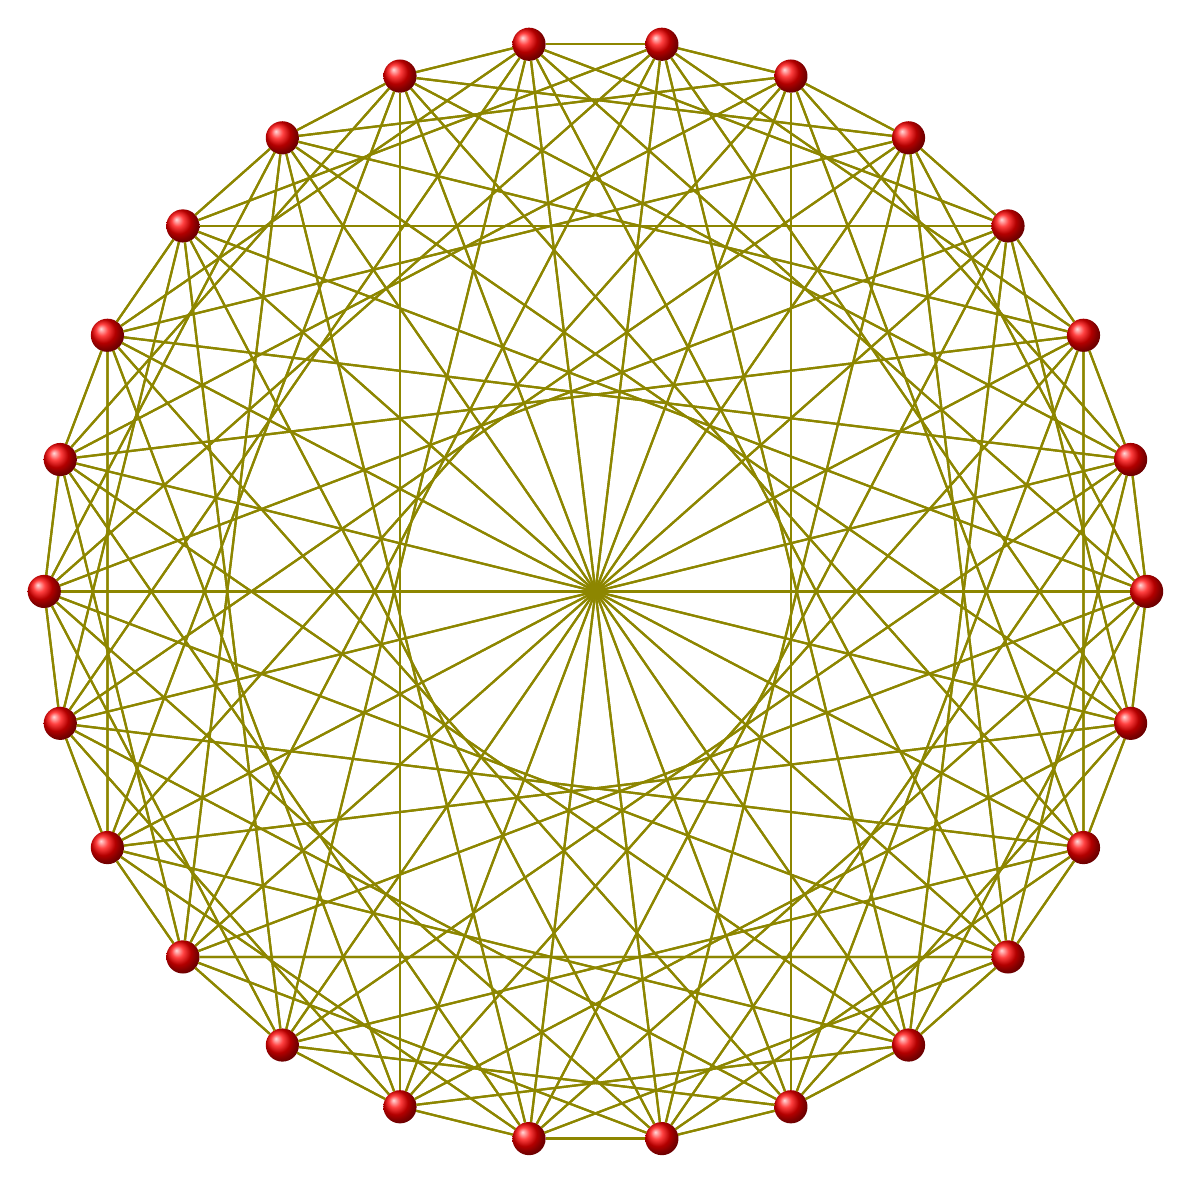
\begin{tikzpicture}
  \GraphInit[vstyle=Art]
  \SetGraphArtColor{red}{olive}
  \grAndrasfai[RA=7]{9}
\end{tikzpicture}
\end{tkzexample}
\end{center}


\endinput

%<–––––––––––––––––––––––––––––––––––––––––––––––––––––––––––––––––––––––––>
\newpage\section{Balaban}\label{balaban}
%<––––––––––––––––––––––––––––––––––––––––––––––––––––––––––––––––––––––––––>
%<––––––––––––––––––––––   Balaban's graph  ––––––––––––––––––––––––––––––––>
%<––––––––––––––––––––––––––––––––––––––––––––––––––––––––––––––––––––––––––>

\begin{NewMacroBox}{grBalaban}{\oarg{options}}

\medskip
From MathWord : \url{http://mathworld.wolfram.com/Balaban10-Cage.html} 

\emph{The Balaban 10-cage is one of the three(3,10)-cage graphs (Read 1998, p. 272). The Balaban (3,10)-cage was the first known example of a 10-cage (Balaban 1973; Pisanski 2001). Embeddings of all three possible (3,10)-cages (the others being the Harries graph and Harries-Wong graph) are given by Pisanski et al. (2001). Several embeddings are illustrated below, with the three rightmost being given by Pisanski and Randić (2000)
It is a Hamiltonian graph and has  Hamiltonian cycles. It has 1003 distinct LCF notations, with four of length two (illustrated above) and 999 of length 1.
\href{http://mathworld.wolfram.com/topics/GraphTheory.html}%
           {\textcolor{blue}{MathWorld}} by \href{http://en.wikipedia.org/wiki/Eric_W._Weisstein}%
           {\textcolor{blue}{E.Weisstein}}
}
\end{NewMacroBox}

\subsection{\tkzname{Balaban graph : first form}}
\begin{center}
\begin{tkzexample}[vbox]
 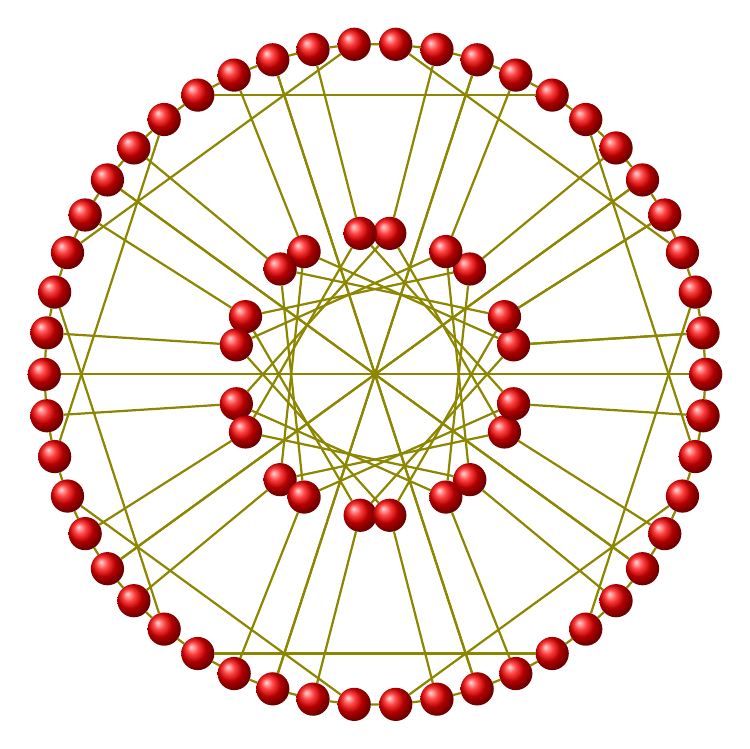
\begin{tikzpicture}[scale=.6]
  \GraphInit[vstyle=Art]
  \SetGraphArtColor{red}{olive}
 \grBalaban[form=1,RA=7,RB=3,RC=3]
 \end{tikzpicture}
\end{tkzexample}

\end{center}


\vfill\newpage
\subsection{\tkzname{Balaban graph : second form}}
\begin{center}
\begin{tkzexample}[vbox]
 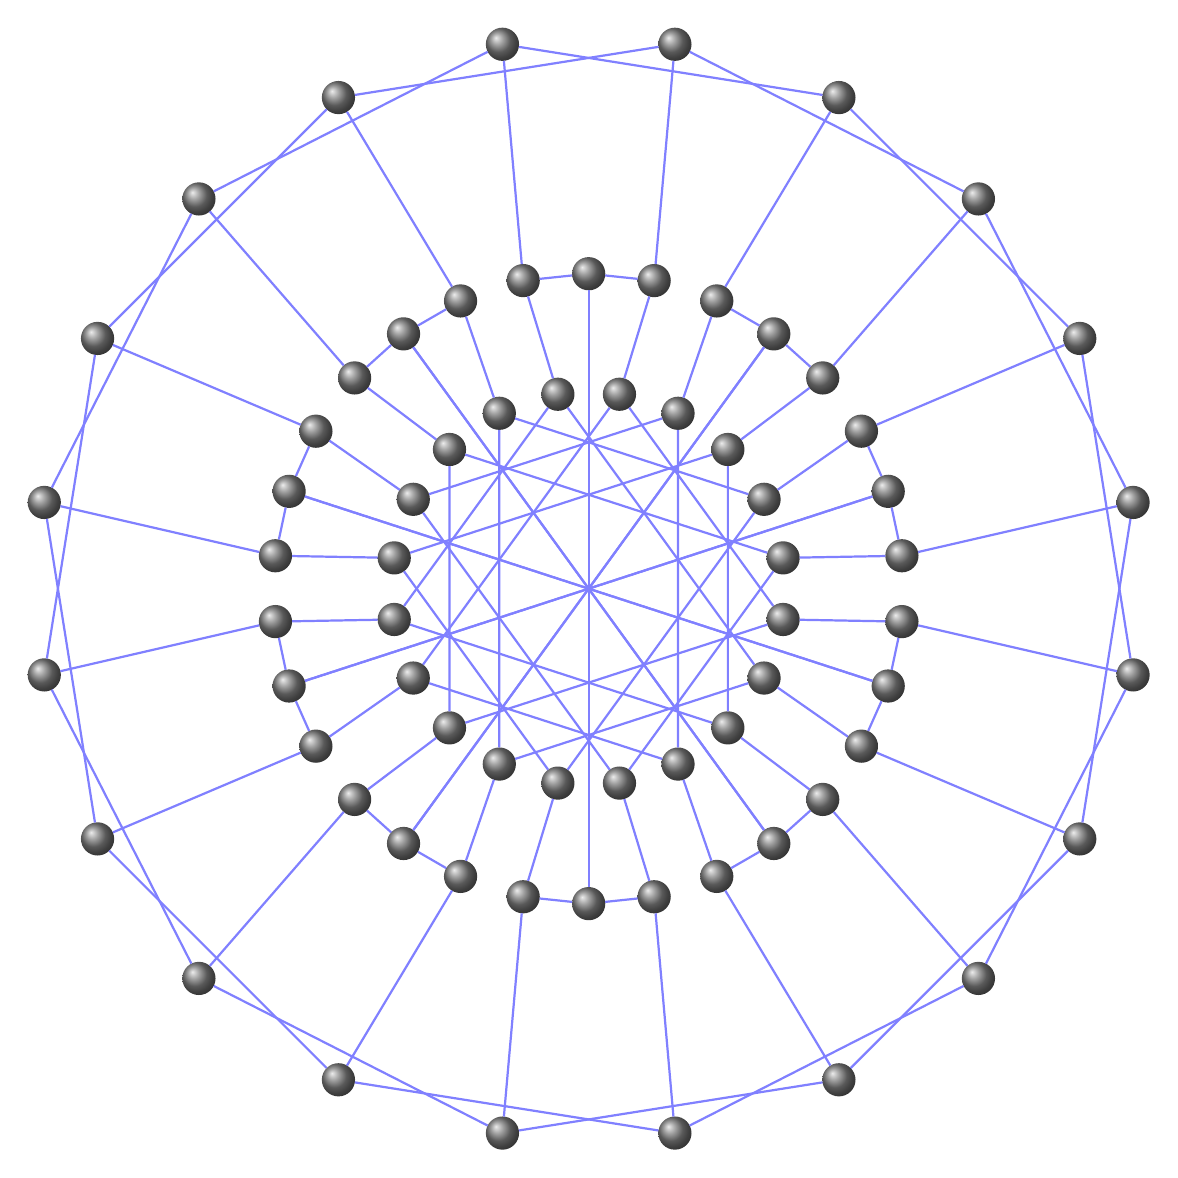
\begin{tikzpicture}
  \GraphInit[vstyle=Art]
  \SetGraphArtColor{gray}{blue!50}
 \grBalaban[form=2,RA=7,RB=7,RC=4,RD=2.5]
 \end{tikzpicture}
\end{tkzexample}

\end{center}

\vfill\newpage
\subsection{\tkzname{Balaban graph : third form} }
\begin{center}
 \begin{tkzexample}[vbox]
  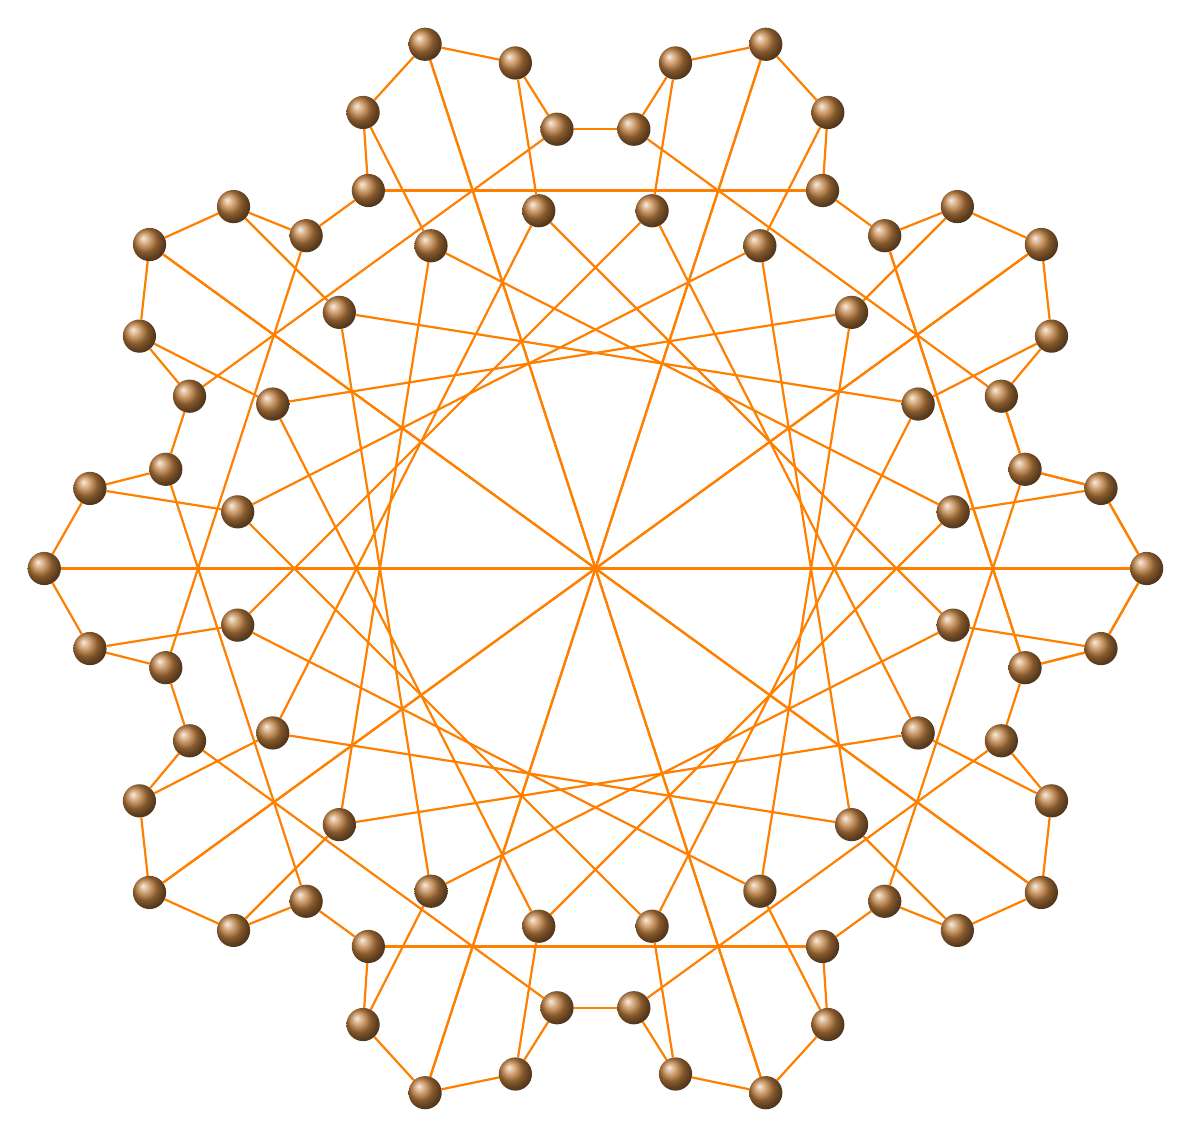
\begin{tikzpicture}
  \GraphInit[vstyle=Art]
  \SetGraphArtColor{brown}{orange}
  \grBalaban[form=3,RA=7,RB=6.5,RC=5.6,RD=5.6,RE=4.6]
  \end{tikzpicture}
 \end{tkzexample}

\end{center}


\vfill\newpage

\subsection{\tkzname{Balaban graph : Balaban 11-Cage}}


The Balaban 11-cage is the unique 11-cage graph, discovered by Balaban (1973) and proven unique by McKay and Myrvold (2003). It has 112 vertices, 168 edges, girth 11 (by definition),  diameter 8 and chromatic number 3.


\begin{center}
\begin{tkzexample}[vbox]
 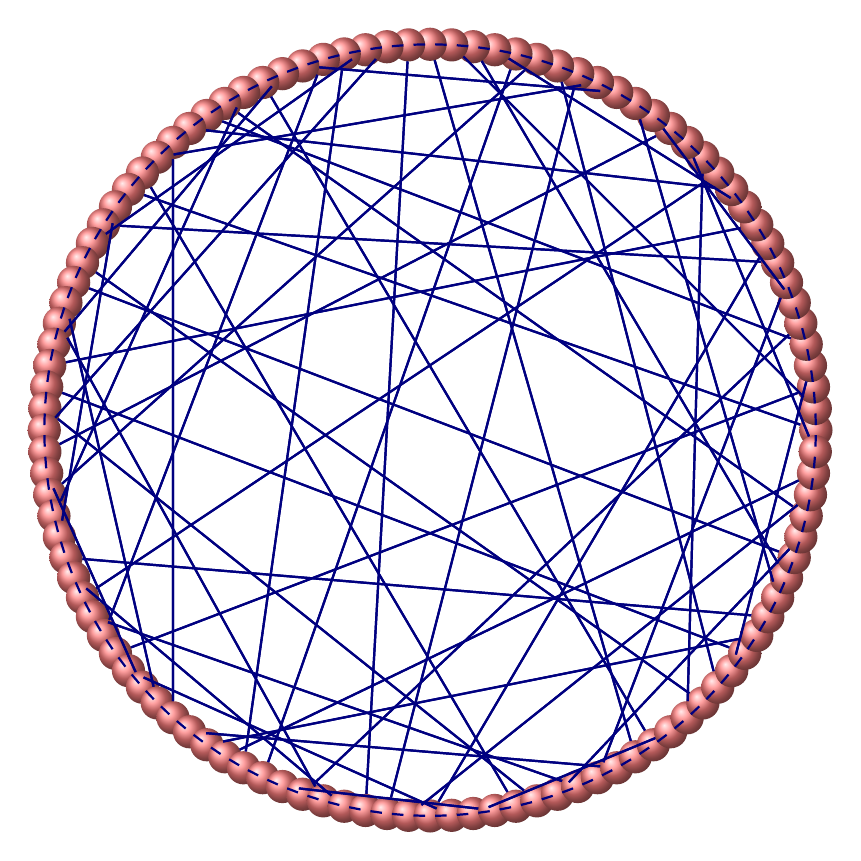
\begin{tikzpicture}[scale=.7]
  \renewcommand*{\VertexInnerSep}{3pt}
  \renewcommand*{\VertexLineWidth}{0.4pt}
  \GraphInit[vstyle=Art]
  \SetGraphArtColor{red!50}{blue!50!black}
 \grLCF[Math,RA=7]{%
 44,26,-47,-15,35,-39,11,-27,38,-37,43,14,28,51,-29,-16,41,-11,%
 -26,15,22,-51,-35,36,52,-14,-33,-26,-46,52,26,16,43,33,-15,%
  17,-53,23,-42,-35,-28,30,-22, 45,-44,16,-38,-16,50,-55,20,28,%
  -17,-43,47, 34,-26,-41,11,-36,-23,-16,41,17,-51,26,-33,47,17,%
  -11,-20 ,-30,21,29,36,-43,-52,10,39,-28,-17,-52,51,26,37,-17,%
  10,-10,-45,-34,17,-26,27,-21,46,53,-10,29,-50,35,15,-47,-29,-41,%
  26,33,55,-17,42,-26,-36,16}{1}
 \end{tikzpicture}
\end{tkzexample}

\end{center}




\endinput
\newpage\section{Complete BiPartite Graph}\label{bipart}
%<––––––––––––––––––––––––––––––––––––––––––––––––––––––––––––––––––––––––––>
%<––––––––––––––––––––––  Complete BiPartite graph  ––––––––––––––––––––––––>
%<––––––––––––––––––––––––––––––––––––––––––––––––––––––––––––––––––––––––––>
\begin{NewMacroBox}{grCompleteBipartite}{\oarg{options}\var{$p$}\var{$q$}}

\medskip
From MathWord : \url{http://mathworld.wolfram.com/CompleteBipartiteGraph.html}

\emph{A complete bipartite graph is a bipartite graph (i.e., a set of graph vertices decomposed into two disjoint sets such that no two graph vertices within the same set are adjacent) such that every pair of graph vertices in the two sets are adjacent. If there are $p$ and $q$ graph vertices in the two sets, the complete bipartite graph (sometimes also called a complete bigraph) is denoted $K_{p,q}$ . The below figures show $K_{3,2}$ and $K_{3,3}$. $K_{3,3}$ is also known as the utility graph (and the circulant graph $Ci_{1,3}(6)$), and is the unique 4-cage graph.} 
\href{http://mathworld.wolfram.com/topics/GraphTheory.html}%
           {\textcolor{blue}{MathWorld}} by \href{http://en.wikipedia.org/wiki/Eric_W._Weisstein}%
           {\textcolor{blue}{E.Weisstein}}

\medskip
From Wikipedia : \url{http://en.wikipedia.org/wiki/Complete_bipartite_graph}

\emph{In the mathematical field of graph theory, a complete bipartite graph or biclique is a special kind of bipartite graph where every vertex of the first set is connected to every vertex of the second set. the graph $K_{1,3}$ is also called a claw.}
\end{NewMacroBox}

\subsection{\tkzname{Complete bipartite graphs $K_{3,2}$ and $K_{3,3}$} }
 %G=LCF_graph(6,[3,-3],3)   
\begin{center}
\begin{tkzexample}[vbox]
 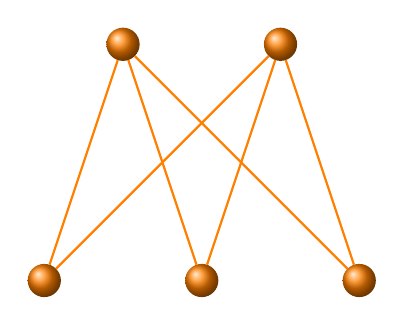
\begin{tikzpicture}
   \GraphInit[vstyle=Art]
   \grCompleteBipartite[RA=2,RB=2,RS=3]{3}{2}
\end{tikzpicture}\hspace*{2cm}
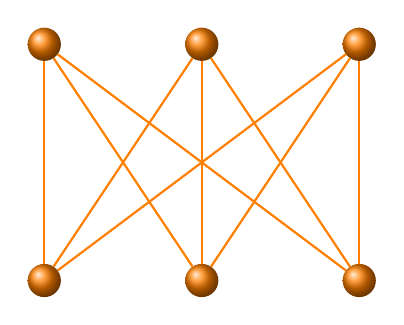
\begin{tikzpicture}
   \GraphInit[vstyle=Art]
   \grCompleteBipartite[RA=2,RB=2,RS=3]{3}{3}
 \end{tikzpicture}
\end{tkzexample}
\end{center}

\subsection{\tkzname{Complete bipartite graphs $K_{3,5}$}}
\begin{center}
\begin{tkzexample}[vbox] 
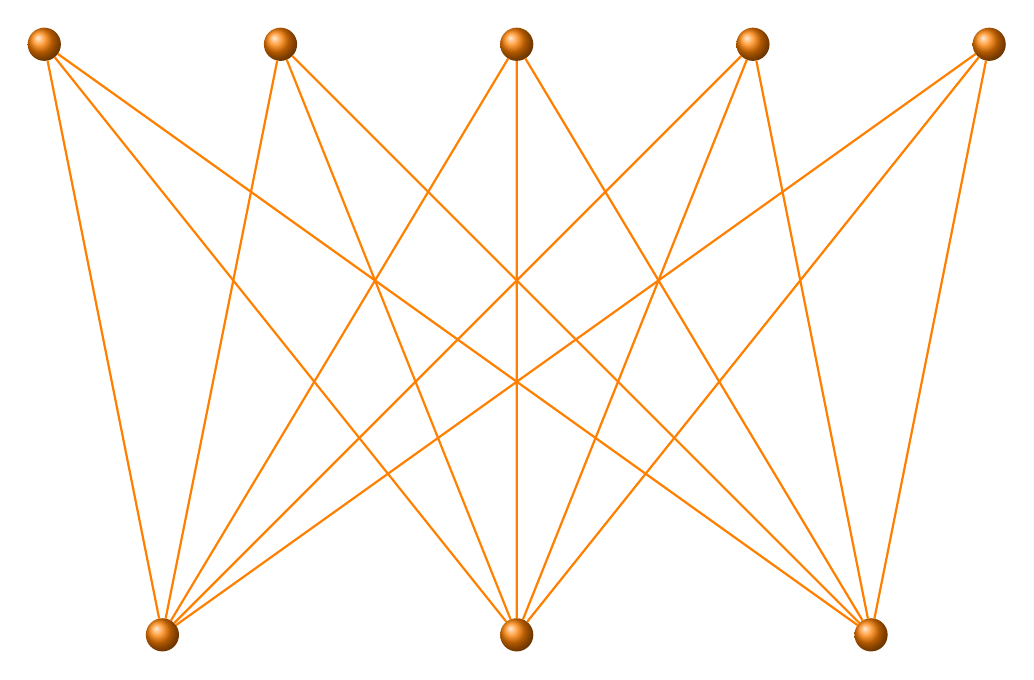
\begin{tikzpicture}[scale=1.5]
  \GraphInit[vstyle=Art]
  \grCompleteBipartite[RA=3,RB=2,RS=5]{3}{5}
\end{tikzpicture}
\end{tkzexample}
\end{center} 

\vfill\newpage

\subsection{\tkzname{Complete bipartite graph : $K_{18,18}$ }}

The complete bipartite graph  illustrated below plays an important role in the novel Foucault's Pendulum by Umberto Eco.

\href{http://mathworld.wolfram.com/CycleGraph.html}%
           {\textcolor{blue}{MathWorld}} by \href{http://en.wikipedia.org/wiki/Eric_W._Weisstein}%
           {\textcolor{blue}{E.Weisstein}}

\vfill
\begin{center}
\begin{tkzexample}[vbox]
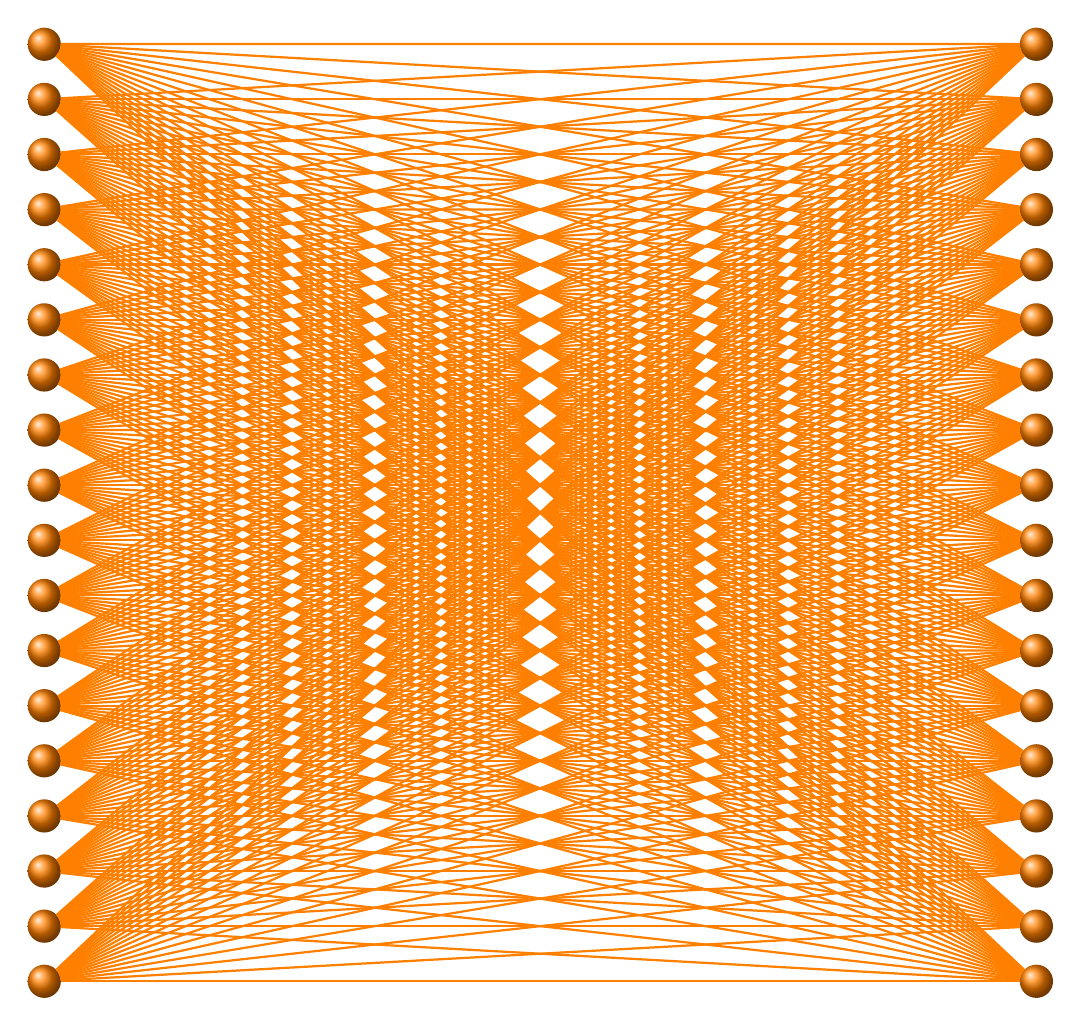
\begin{tikzpicture}[rotate=90,scale=1.4]
  \GraphInit[vstyle=Art]
  \grCompleteBipartite[RA=0.5,RB=0.5,RS=9]{18}{18}
\end{tikzpicture}
\end{tkzexample}
\end{center}

\vfill\newpage
A complete bipartite graph $K_{n,n}$ is a circulant graph (if the order is equal to $2n$ then $L=1,3,\dots,n$).
The code is on the next page

\bigskip
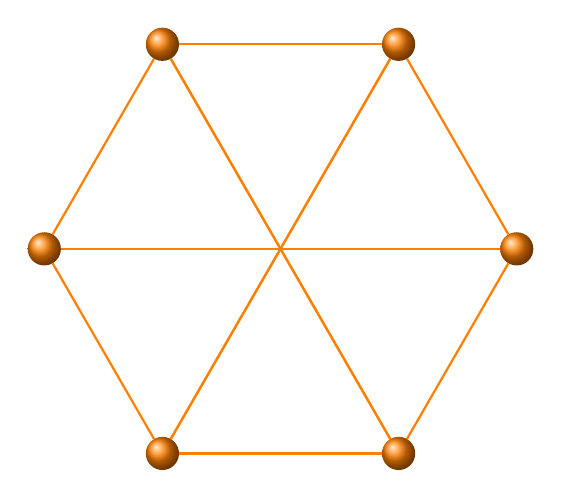
\begin{tikzpicture}
  \GraphInit[vstyle=Art]
  \grCirculant[RA=3]{6}{1,3}
\end{tikzpicture}\hspace*{12pt} 
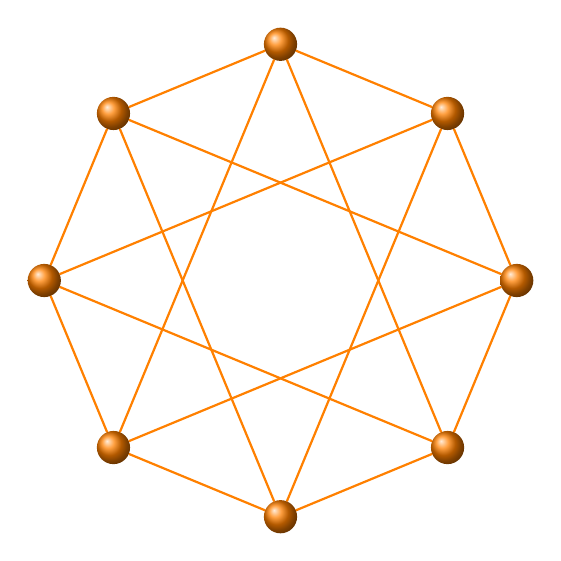
\begin{tikzpicture}
  \GraphInit[vstyle=Art]
  \grCirculant[RA=3]{8}{1,3}
\end{tikzpicture}

\vspace*{12pt} 
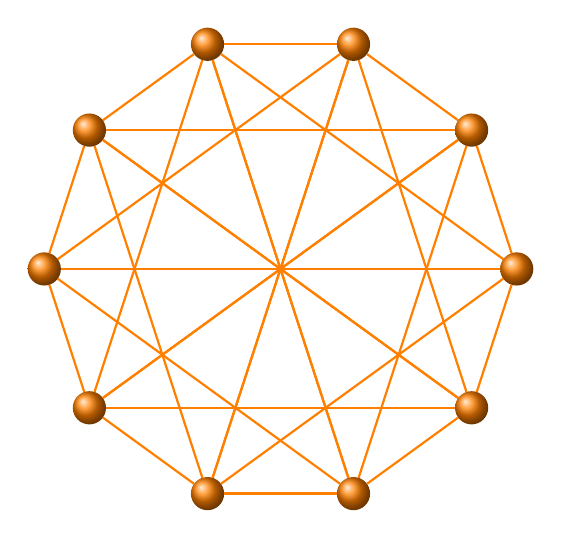
\begin{tikzpicture}
  \GraphInit[vstyle=Art]
  \grCirculant[RA=3]{10}{1,3,5}
\end{tikzpicture}\hspace*{12pt} 
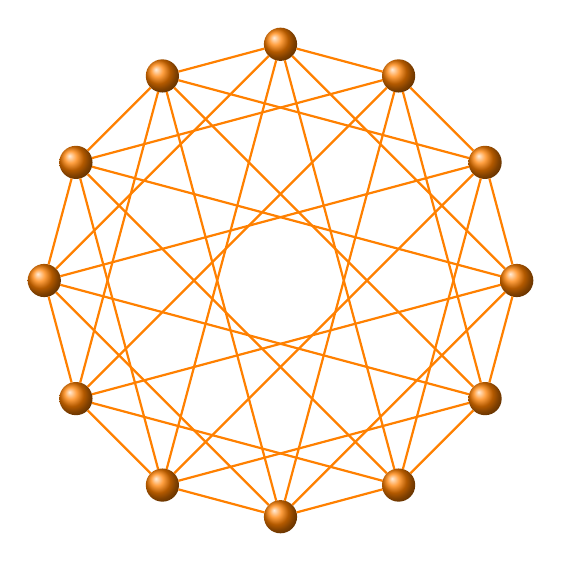
\begin{tikzpicture}
  \GraphInit[vstyle=Art]
  \grCirculant[RA=3]{12}{1,3,5}
\end{tikzpicture}

\vspace*{12pt}
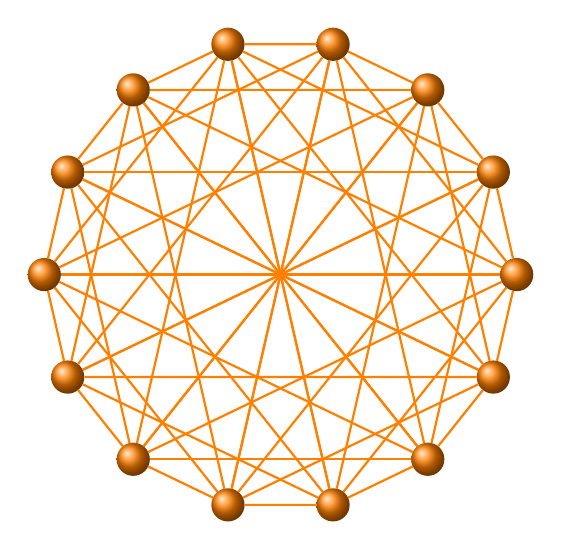
\begin{tikzpicture}
 \GraphInit[vstyle=Art]
 \grCirculant[RA=3]{14}{1,3,5,7}
\end{tikzpicture}\hspace*{12pt} 
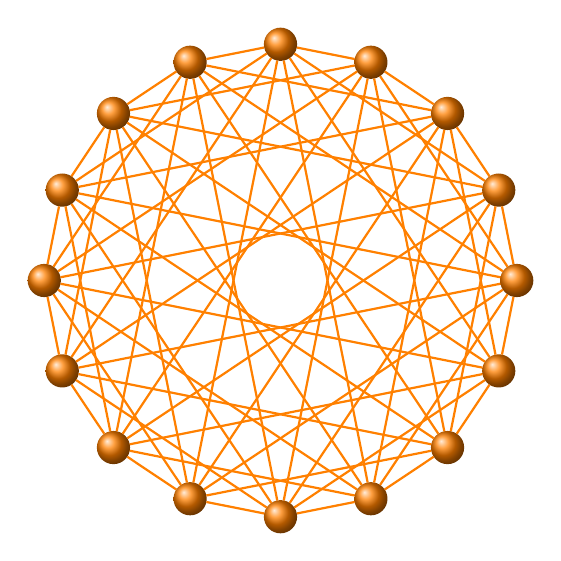
\begin{tikzpicture}
  \GraphInit[vstyle=Art]
 \grCirculant[RA=3]{16}{1,3,5,7}
\end{tikzpicture} 

\vfill\newpage
\begin{tkzexample}[code only]
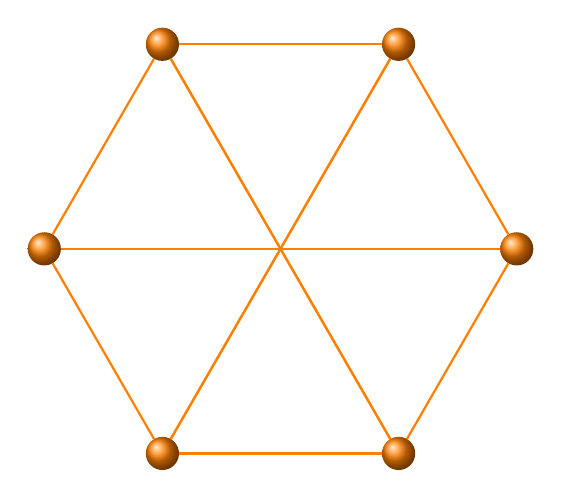
\begin{tikzpicture}
  \GraphInit[vstyle=Art]
  \grCirculant[RA=3]{6}{1,3}
\end{tikzpicture}\hspace*{12pt} 
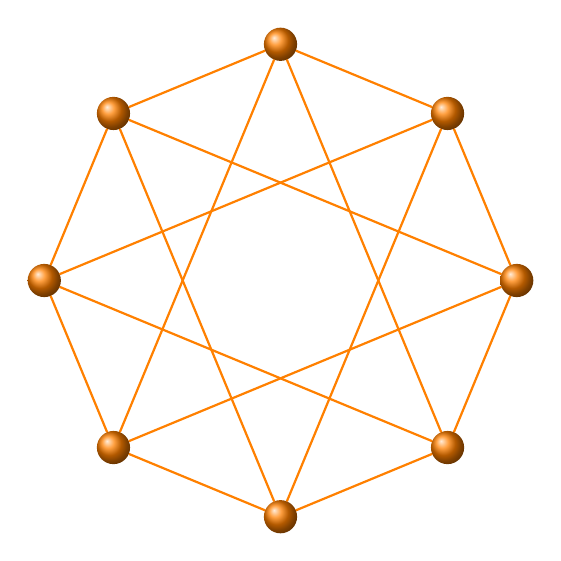
\begin{tikzpicture}
  \GraphInit[vstyle=Art]
  \grCirculant[RA=3]{8}{1,3}
\end{tikzpicture}

\vspace*{12pt} 
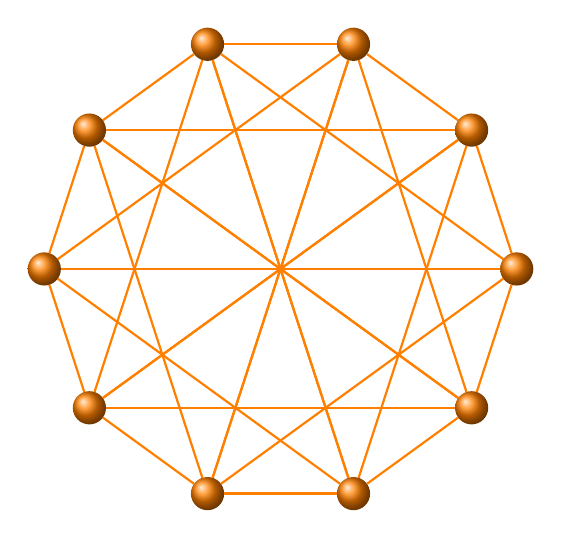
\begin{tikzpicture}
  \GraphInit[vstyle=Art]
  \grCirculant[RA=3]{10}{1,3,5}
\end{tikzpicture}\hspace*{12pt} 
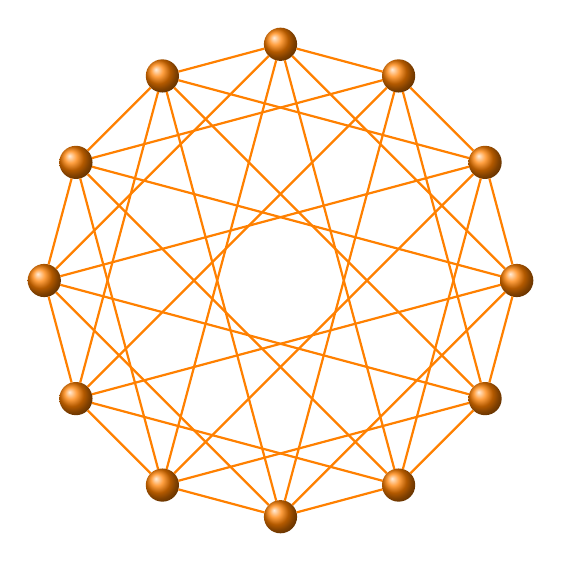
\begin{tikzpicture}
  \GraphInit[vstyle=Art]
  \grCirculant[RA=3]{12}{1,3,5}
\end{tikzpicture}

\vspace*{12pt}
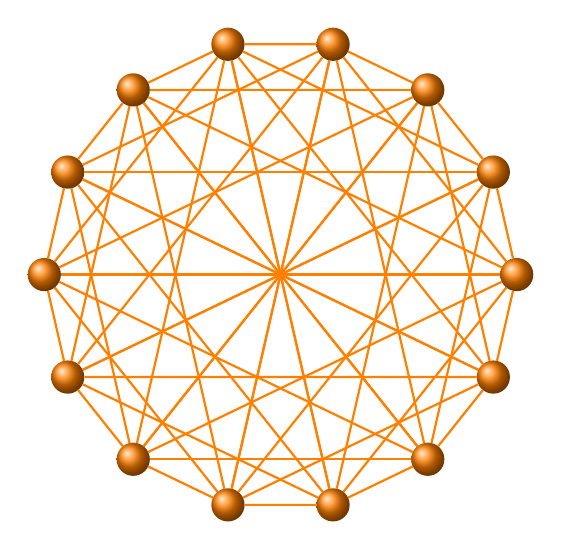
\begin{tikzpicture}
       \GraphInit[vstyle=Art]
\grCirculant[RA=3]{14}{1,3,5,7}
\end{tikzpicture}\hspace*{12pt} 
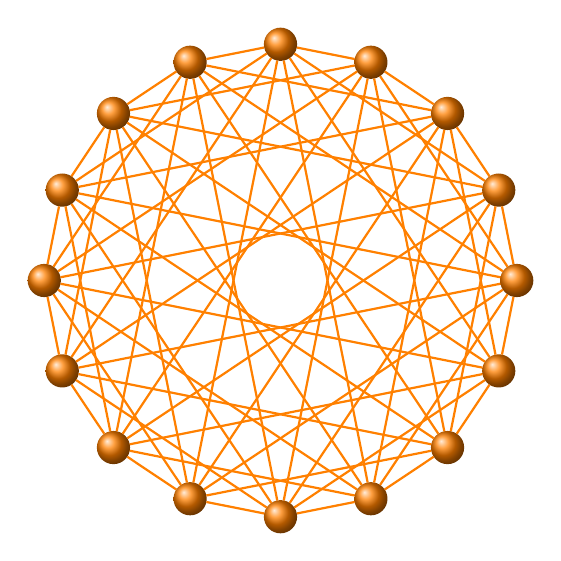
\begin{tikzpicture}
       \GraphInit[vstyle=Art]
\grCirculant[RA=3]{16}{1,3,5,7}
\end{tikzpicture}
\end{tkzexample}


\endinput


\newpage\section{Bull}
%<–––––––––––––––––––––––––––––––––––––––––––––––––––––––––––––––––––––––––>
%                               Bull
%<–––––––––––––––––––––––––––––––––––––––––––––––––––––––––––––––––––––––––>
The bull graph, 5 vertices, 5 edges, resembles to the head of a bull if drawn properly. 
The bull graph is a simple graph on 5 nodes and 5 edges whose name derives from its resemblance to a schematic illustration of a bull 

\begin{center}
\begin{tkzexample}[vbox]
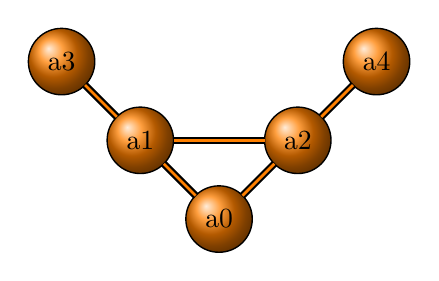
\begin{tikzpicture}[node distance=4cm]
  \GraphInit[vstyle=Shade]
  \Vertex{a0}
  \NOEA(a0){a2}
  \NOEA(a2){a4}
  \NOWE(a0){a1}
  \NOWE(a1){a3}
  \Edges(a0,a1,a3)
  \Edges(a0,a2,a4)
  \Edge(a1)(a2)
 \end{tikzpicture}
\end{tkzexample} 
\end{center}

\endinput

\newpage\section{Cage}\label{cage}
%<––––––––––––––––––––––––––––––––––––––––––––––––––––––––––––––––––––––––––>
%<––––––––––––––––––––   Cage                –––––––––––––––––––––––––––––––>
%<––––––––––––––––––––––––––––––––––––––––––––––––––––––––––––––––––––––––––>
\begin{NewMacroBox}{Cage Graphs}{}

\medskip
From Wikipedia  \url{http://en.wikipedia.org/wiki/Cage_(graph_theory)}\\
\emph{In the mathematical area of graph theory, a cage is a regular graph that has as few vertices as possible for its girth.\\
Formally, an $(r,g)$-graph is defined to be a graph in which each vertex has exactly $r$ neighbors, and in which the shortest cycle has length exactly $g$. It is known that an $(r,g)$-graph exists for any combination of $r \geq 2$ and $g \geq 3$. An $(r,g)$-cage is an $(r,g)$-graph with the fewest possible number of vertices, among all $(r,g)$-graphs.}

\medskip
From MathWorld \url{http://mathworld.wolfram.com/CageGraph.html}\\
\emph{A $(r,g)$-cage graph is a $v$-regular graph of girth $g$ having the minimum possible number of nodes. When $v$ is not explicitly stated, the term "$g$-cage" generally refers to a $(3,g)$-cage.}
\href{http://mathworld.wolfram.com/topics/GraphTheory.html}%
           {\textcolor{blue}{MathWorld}} by \href{http://en.wikipedia.org/wiki/Eric_W._Weisstein}%
           {\textcolor{blue}{E.Weisstein}}

\medskip
Examples :

\medskip
\begin{tabular}{ll}
  \bottomrule
$(r,g)$ & Names                                                     \\
\midrule
$(3,3)$     & complete graph $K_4$                                  \\
$(3,4)$     & complete bipartite graph $K_{3,3}$ Utility Graph\ref{bipart} \\
$(3,5)$     & Petersen graph \ref{petersen}                          \\
$(3,6)$     & Heawood graph  \ref{heawood}                           \\
$(3,7)$     & McGee graph \ref{mcgee}                                \\
$(3,8)$     & Levi graph \ref{levi}                                  \\
$(3,10)$    & Balaban 10-cage     \ref{balaban}                      \\
$(3,11)$    & Balaban 11-cage     \ref{balaban}                      \\
$(3,12)$    & Tutte 12-cage                                          \\
$(4,3)$     & complete graph $K_5$                                   \\
$(4,4)$     & complete bipartite graph $K_{4,4}$ \ref{bipart}          \\
$(4,5)$     & Robertson graph\ref{robertson}                         \\
$(4,6)$     & Wong (1982)\ref{wong}                                  \\
\end{tabular}
\end{NewMacroBox}

\endinput   
\newpage\section{Cocktail Party graph}\label{cocktail}
%<––––––––––––––––––––––––––––––––––––––––––––––––––––––––––––––––––––––––––>
%<–––––––––––––––––––––––––––––   Cocktail Party  –––––––––––––––––––––––––––>
%<––––––––––––––––––––––––––––––––––––––––––––––––––––––––––––––––––––––––––>
\begin{NewMacroBox}{grCocktailParty}{\oarg{options}\var{integer}}

\medskip
From MathWord : \url{http://mathworld.wolfram.com/CocktailPartyGraph.html}  

\emph{The cocktail party graph of order , also called the hyperoctahedral graph (Biggs 1993, p. 17) is the graph consisting of two rows of paired nodes in which all nodes but the paired ones are connected with a graph edge. It is the graph complement of the ladder graph , and the dual graph of the hypercube graph.\hfill\break
This graph arises in the handshake problem. It is a complete n-partite graph that is denoted  by Brouwer et al. (1989, pp. 222-223), and is distance-transitive, and hence also distance-regular.\hfill\break
The cocktail party graph of order  is isomorphic to the circulant graph.}
\href{http://mathworld.wolfram.com/topics/GraphTheory.html}%
           {\textcolor{blue}{MathWorld}} by \href{http://en.wikipedia.org/wiki/Eric_W._Weisstein}%
           {\textcolor{blue}{E.Weisstein}}

\medskip
The Chvátal graph is implemented in \tkzname{tkz-berge} as \tkzcname{grCocktailParty} with two forms.
\end{NewMacroBox}

\subsection{\tkzname{Cocktail Party graph form 1 }}
\tikzstyle{VertexStyle}   = [shape          = circle,
                             shading         = ball,%
                             ball color      = green,%
                             minimum size    = 24pt,%
                             draw]
\SetVertexMath
\tikzstyle{EdgeStyle}     = [thick,%
                             double          = orange,%
                             double distance = 1pt] 
\begin{center}
   \begin{tkzexample}[vbox]
    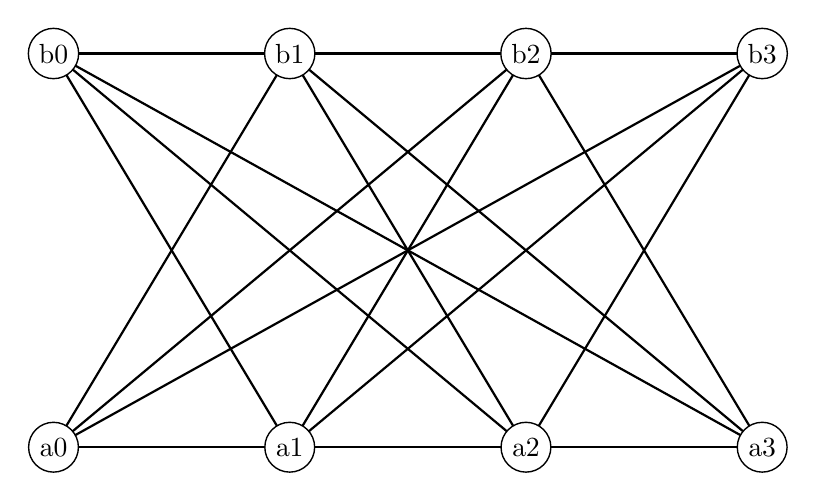
\begin{tikzpicture}
       \grCocktailParty[RA=3,RS=5]{4}
 \end{tikzpicture}
\end{tkzexample} 
\end{center}

\vfill\newpage
\subsection{\tkzname{Cocktail Party graph form 2 }}

\vspace*{2cm}
\begin{center}
   \begin{tkzexample}[vbox]
   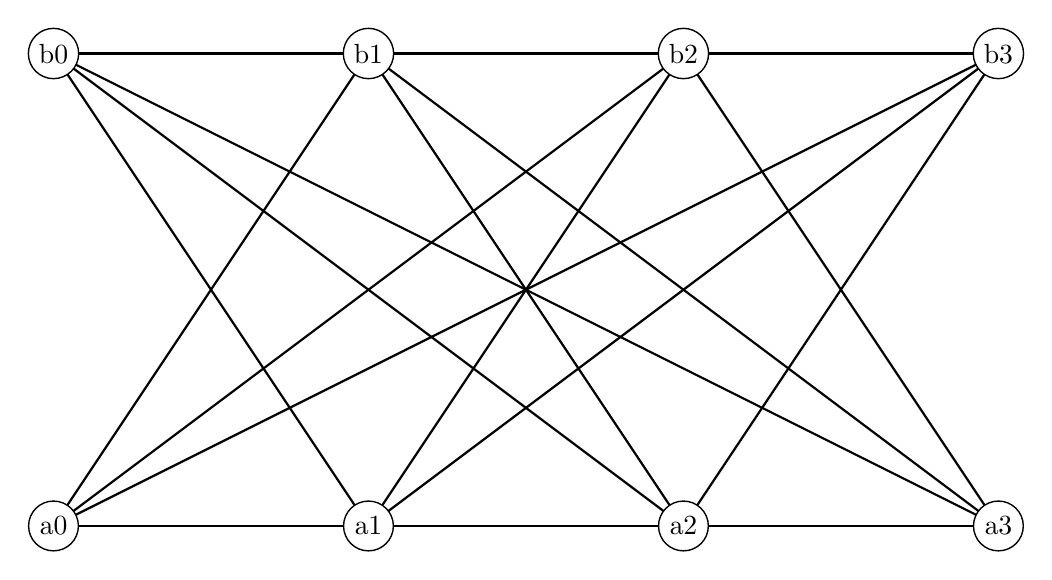
\begin{tikzpicture}
      \grCocktailParty[form=2,RA=4,RS=6]{4}
     \end{tikzpicture}
\end{tkzexample} 
\end{center}
\endinput

\newpage\section{Coxeter}
%<––––––––––––––––––––––––––––––––––––––––––––––––––––––––––––––––––––––––––>
%<–––––––––––––––––––––––––––––    Coxeter  ––––––––––––––––––––––––––––––––>
%<––––––––––––––––––––––––––––––––––––––––––––––––––––––––––––––––––––––––––>
From MathWorld : \url{http://mathworld.wolfram.com/CoxeterGraph.html}

The Coxeter graph is a nonhamiltonian cubic symmetric graph on 28 vertices and 42 edges.


\subsection{\tkzname{Coxeter graph I}}

\bigskip
\begin{center}
\begin{tkzexample}[vbox]
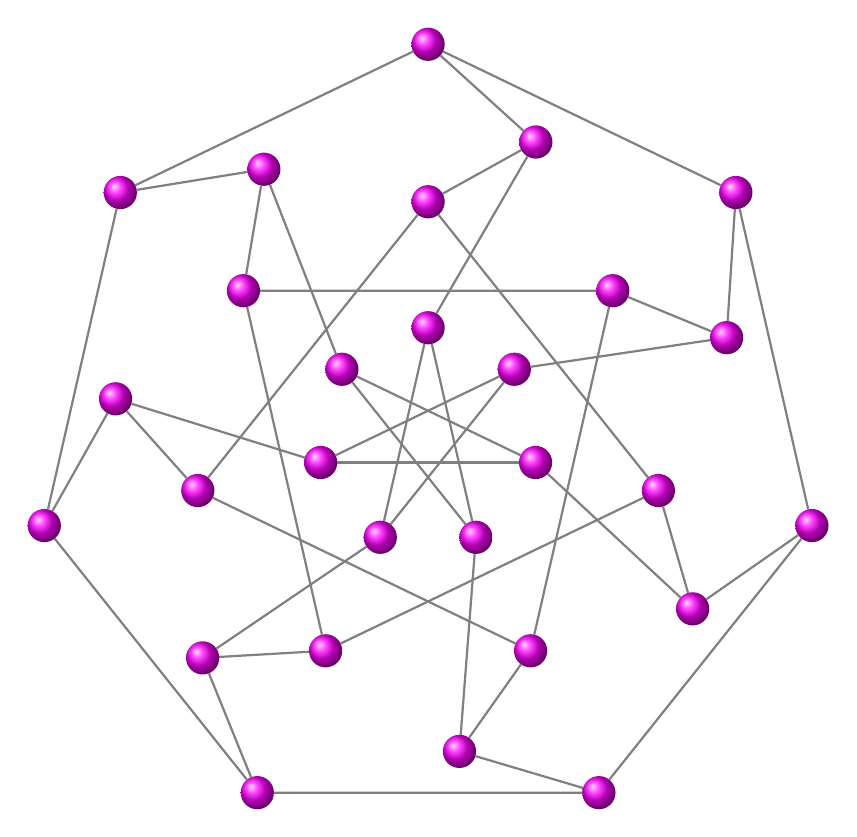
\begin{tikzpicture}[rotate=90,scale=1]
  \GraphInit[vstyle=Art]
  \SetGraphArtColor{magenta}{gray}
  \grCycle[RA=5,prefix=a]{7}
  \begin{scope}[rotate=-20]\grEmptyCycle[RA=4,prefix=b]{7}\end{scope}
  \grCirculant[RA=3,prefix=c]{7}{2}
  \grCirculant[RA=1.4,prefix=d]{7}{3}
  \EdgeIdentity{a}{b}{7} 
  \EdgeIdentity{b}{c}{7} 
  \EdgeIdentity{b}{d}{7} 
 \end{tikzpicture}
\end{tkzexample} 
\end{center}


\vfill\newpage
\subsection{\tkzname{Coxeter graph II}}

\bigskip
\begin{center}
\begin{tkzexample}[vbox]
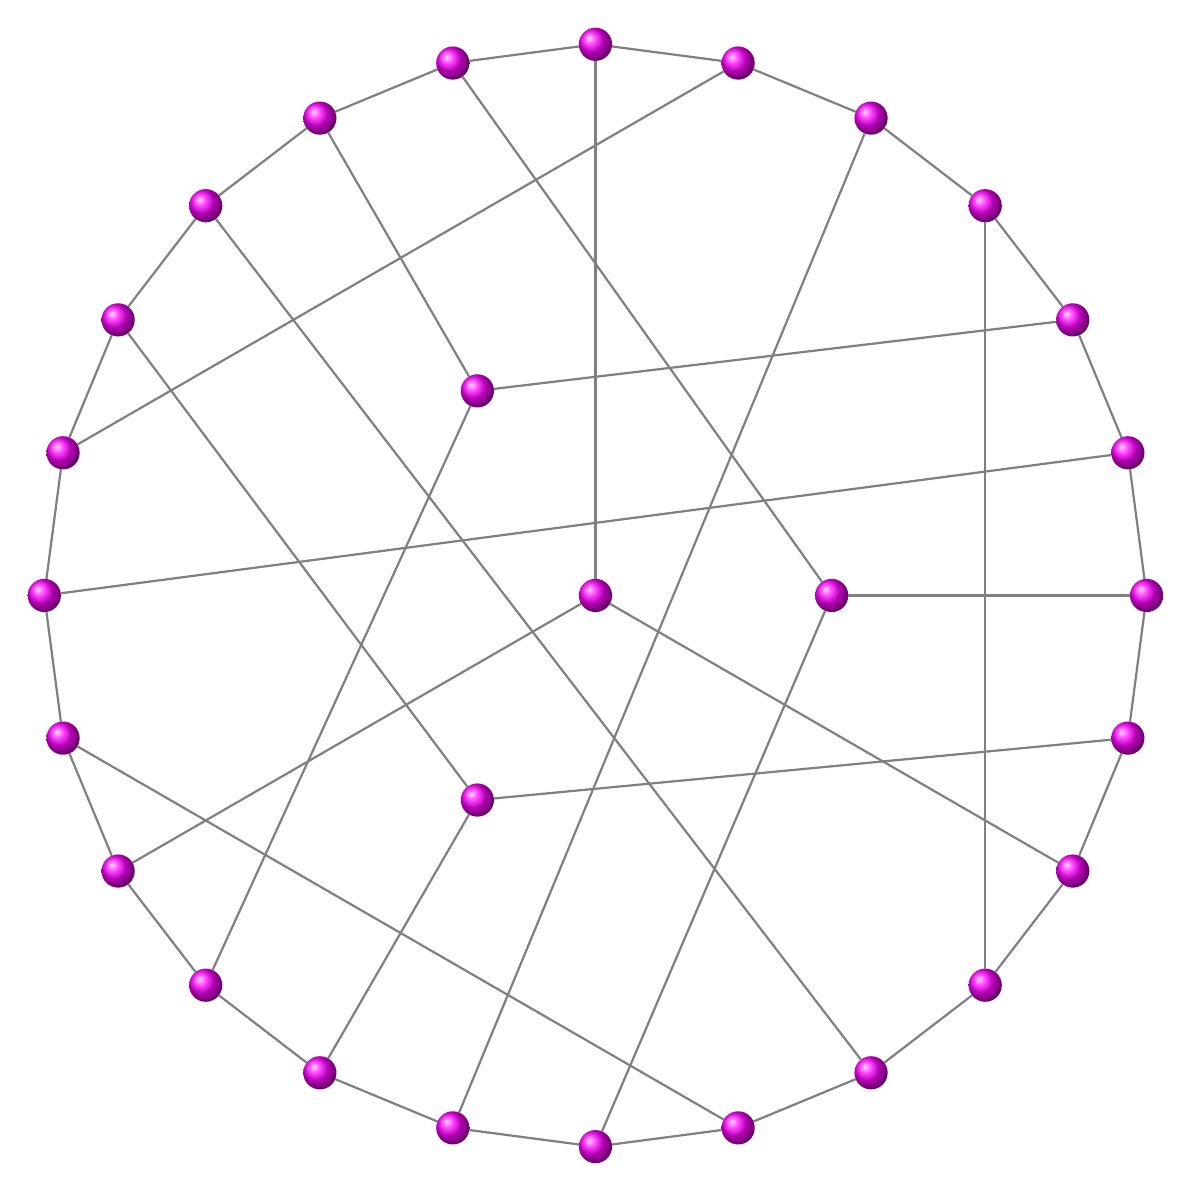
\begin{tikzpicture}
  \GraphInit[vstyle=Art]
  \SetGraphArtColor{magenta}{gray}
  \grCycle[RA=7,prefix=b]{24}
  \grEmptyStar[RA=3,prefix=a]{4}
  \EdgeDoubleMod{a}{3}{0}{1}{b}{24}{0}{8}{2}
  \EdgeDoubleMod{a}{3}{0}{1}{b}{24}{7}{8}{2}
  \EdgeDoubleMod{a}{3}{0}{1}{b}{24}{18}{8}{2}
  \EdgeDoubleMod{a}{4}{3}{0}{b}{24}{22}{8}{2}
  \EdgeInGraphMod*{b}{24}{6}{5}{8}
  \EdgeInGraphMod*{b}{24}{11}{1}{8}
 \end{tikzpicture}
\end{tkzexample} 
\end{center}


\vfill\newpage

\subsection{\tkzname{Coxeter graph III}}

\bigskip
\begin{center}
\begin{tkzexample}[vbox]
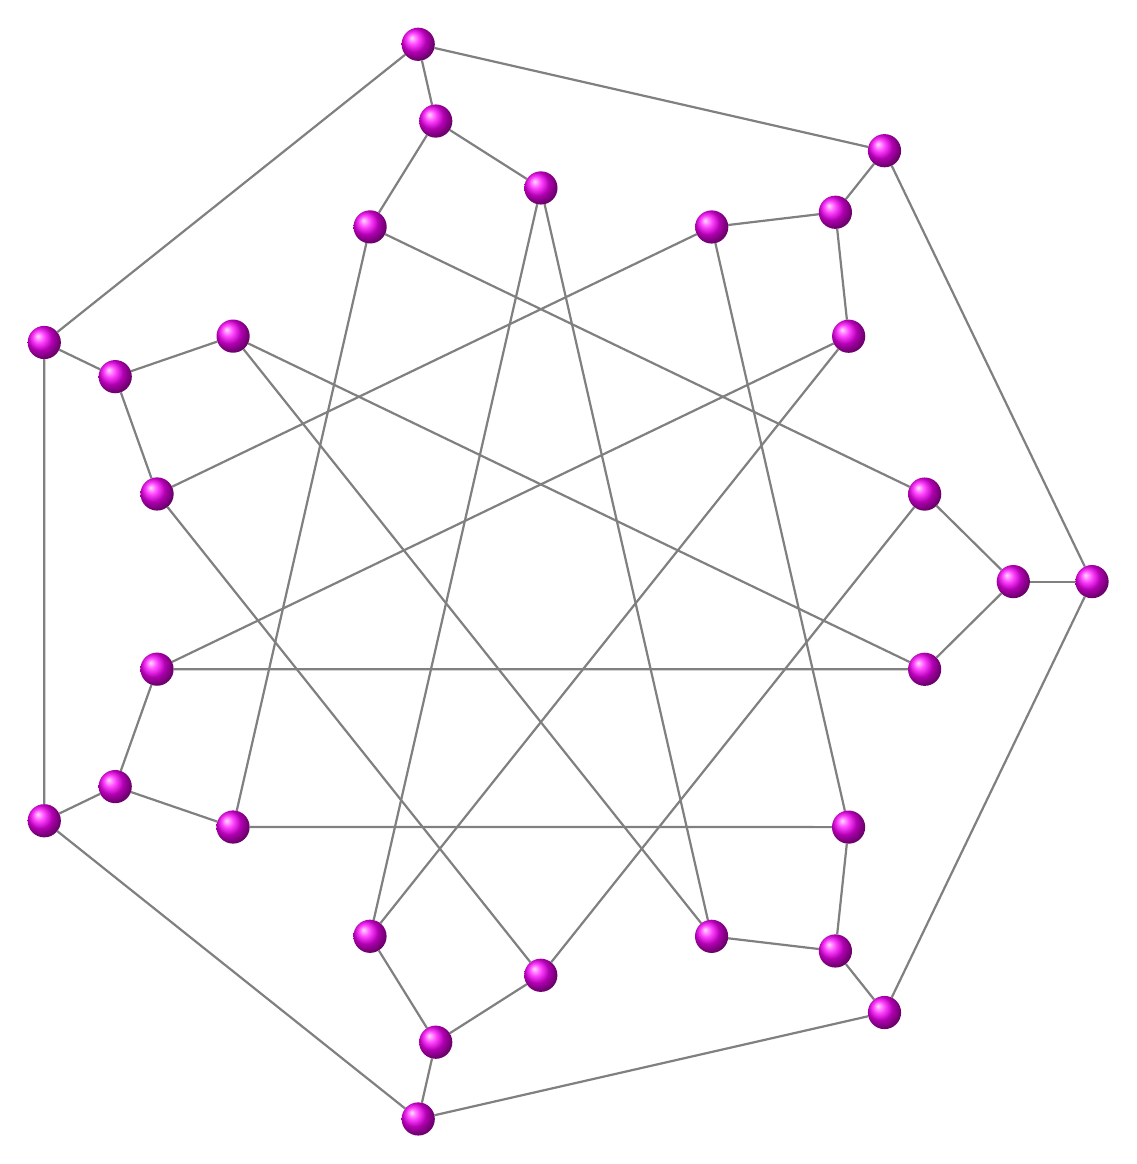
\begin{tikzpicture}
  \GraphInit[vstyle=Art]
  \SetGraphArtColor{magenta}{gray}
  \grCycle[RA=7,prefix=c]{7}
  \grEmptyCycle[RA=6,prefix=b]{7}
  \begin{scope}[rotate=12.85]\grEmptyCycle[RA=5,prefix=a]{14}\end{scope}
  \EdgeIdentity{b}{c}{7}
  \EdgeDoubleMod{b}{7}{0}{1}{a}{14}{0}{2}{6}
  \EdgeDoubleMod{b}{7}{0}{1}{a}{14}{13}{2}{6}
  \EdgeInGraphModLoop{a}{14}{4}{0}{0}
  \EdgeInGraphModLoop{a}{14}{6}{1}{1}
 \end{tikzpicture}
\end{tkzexample} 
\end{center}

%<––––––––––––––––––––––––––––––––––––––––––––––––––––––––––––––––––––––––––>
%<––––––––––––––––––––   Tutte-Coxeter graph    ––––––––––––––––––––––––––––>
%<––––––––––––––––––––––––––––––––––––––––––––––––––––––––––––––––––––––––––>

\vfill\newpage
\subsection{\tkzname{Tutte-Coxeter graph I}}

\tikzstyle{VertexStyle} = [very thin,draw,
                           shape                =  circle,
                           color                =  white,
                           fill                 =  black,
                           inner sep            =  0pt,
                           minimum size         =  18pt]
\tikzstyle{EdgeStyle}   = [thick,
                           double               = brown,
                           double distance      = 1pt]

\bigskip
\begin{center}
\begin{tkzexample}[vbox]
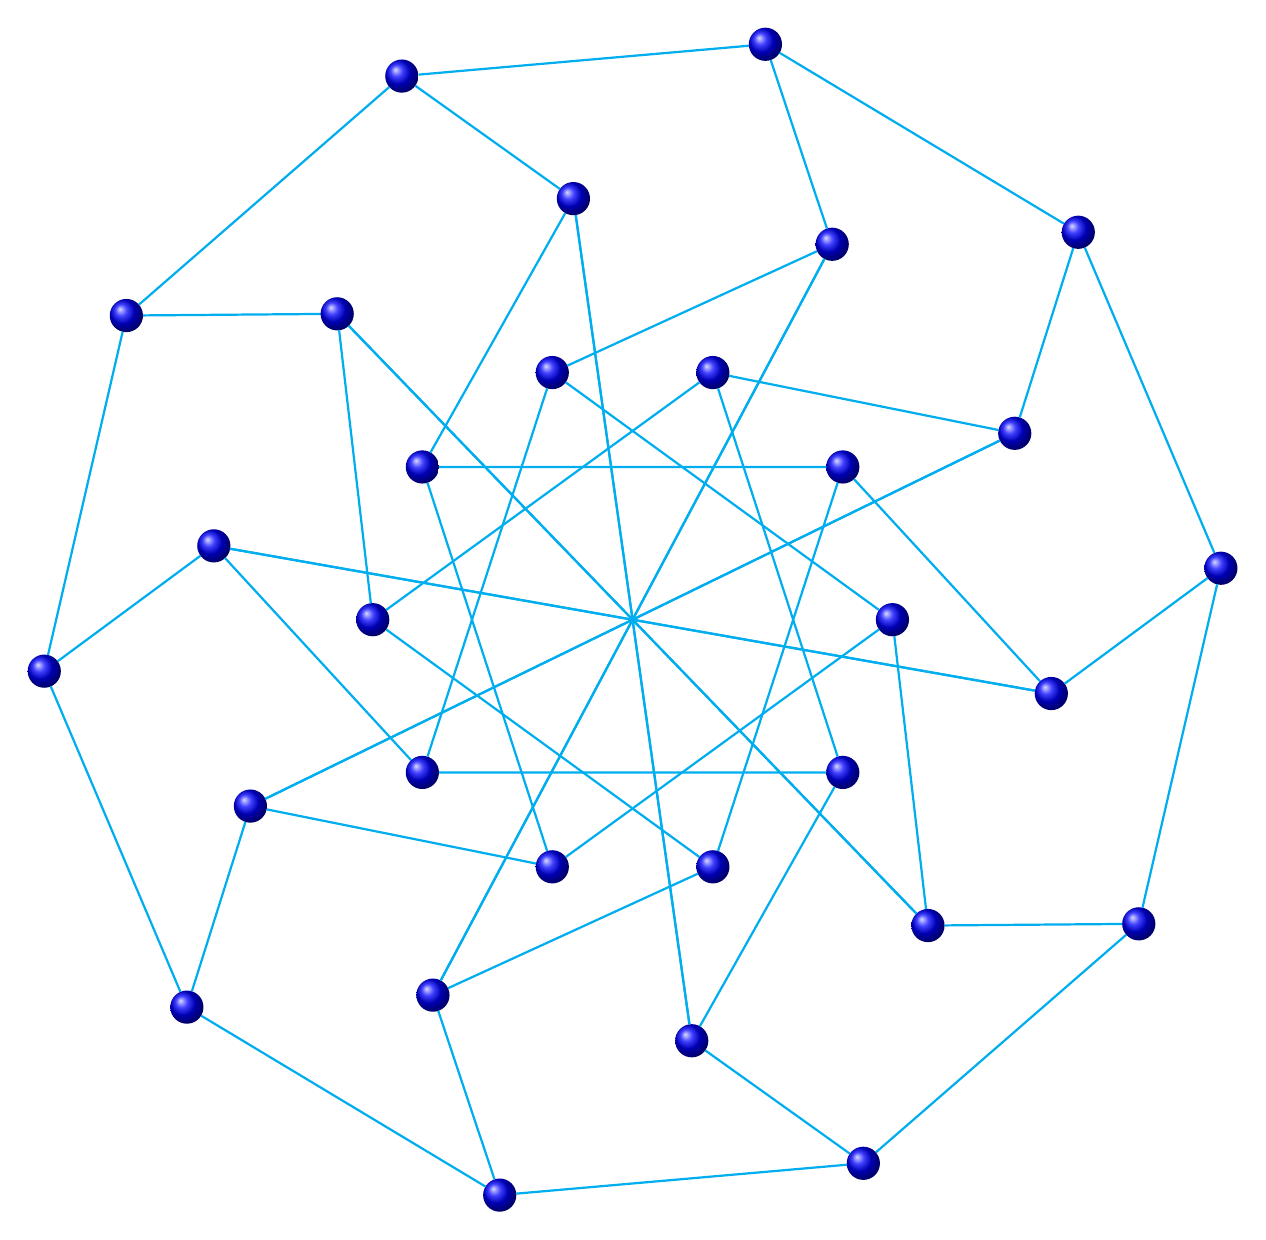
\begin{tikzpicture}[scale=3]
  \GraphInit[vstyle=Art]
  \SetGraphArtColor{blue}{cyan}
  \begin{scope}[rotate=5]\grCycle[RA=2.5,prefix=a]{10}\end{scope}
  \begin{scope}[rotate=-10]\grCirculant[RA=1.8,prefix=b]{10}{5}\end{scope}
  \begin{scope}[rotate=36]\grCirculant[RA=1.1,prefix=c]{10}{3}\end{scope}
  \EdgeIdentity{a}{b}{10} 
  \EdgeIdentity{b}{c}{10} 
 \end{tikzpicture}
\end{tkzexample} 
\end{center}
% 

\vfill\newpage
\subsection{\tkzname{Tutte-Coxeter graph II}}

\bigskip
\begin{center}
\begin{tkzexample}[vbox]
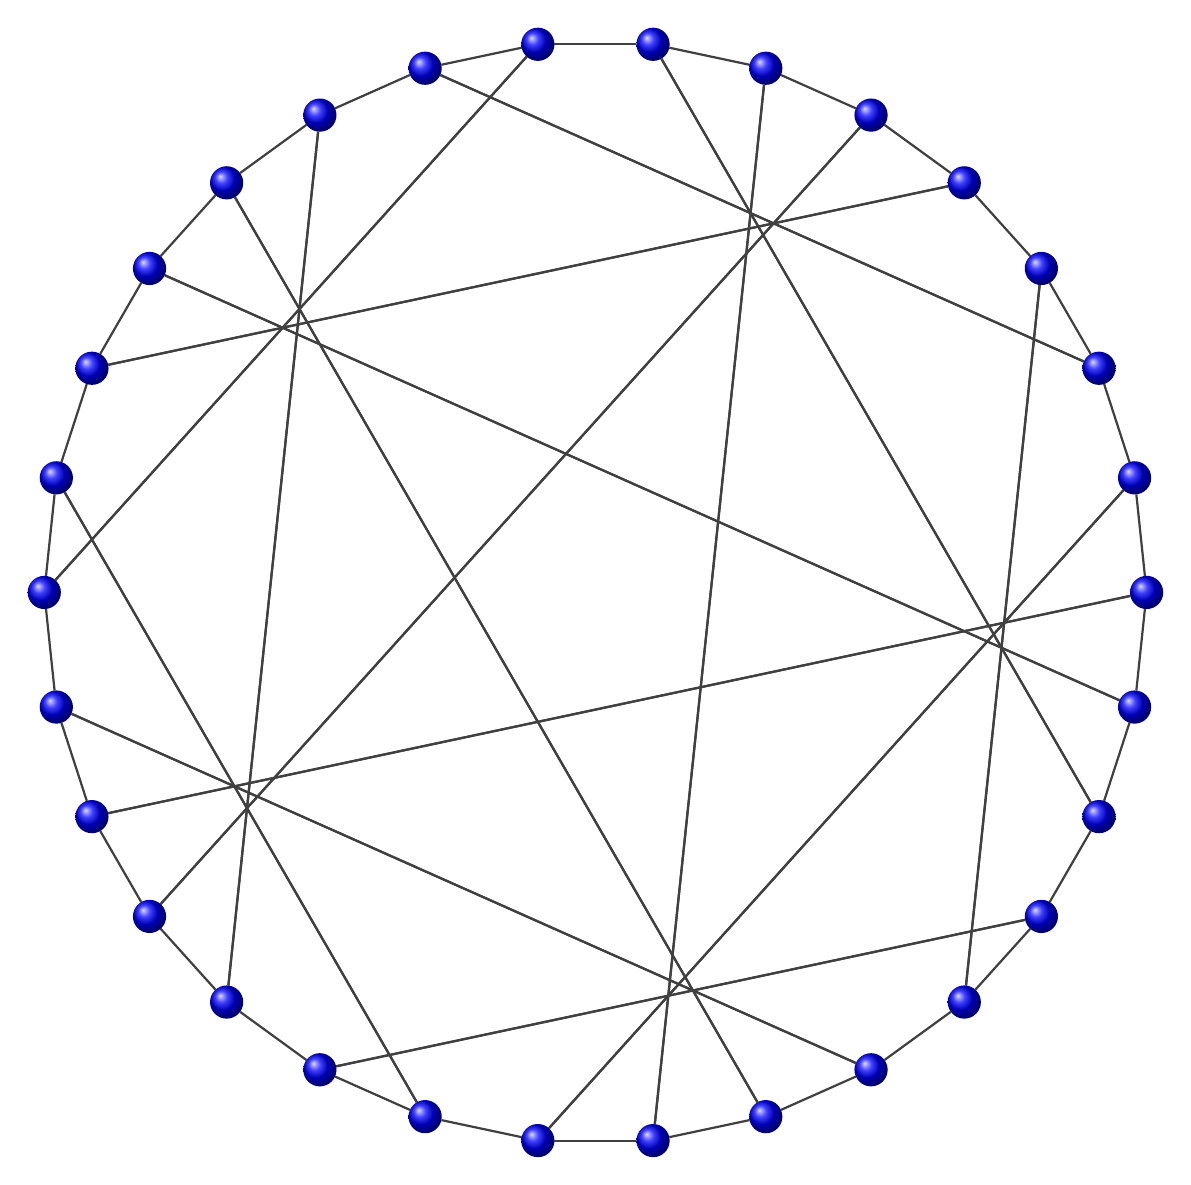
\begin{tikzpicture}
     \GraphInit[vstyle=Art]
     \SetGraphArtColor{blue}{darkgray}
     \grLCF[RA=7]{-13,-9,7,-7,9,13}{5}
 \end{tikzpicture}
\end{tkzexample} 
\end{center}


\endinput
\newpage\section{Chvatal}
%<–––––––––––––––––––––––––––––––––––––––––––––––––––––––––––––––––––––––––>
\begin{NewMacroBox}{grChvatal}{\oarg{options}}

\medskip
From Wikipedia : \url{http://en.wikipedia.org/wiki/Václav_Chvátal} 

\emph{Chvátal first learned of graph theory in 1964, on finding a book by Claude Berge in a Pilsen bookstore, and his first mathematical publication, at the age of 19, concerned directed graphs that cannot be mapped to themselves by any nontrivial graph homomorphism.\hfill\break
Gallery Theorem—which determines the number of guards required to survey the 
walls of a polygonal art gallery (and has prompted much research), and constructed the smallest triangle-free 4-chromatic 4-regular graph, a beautiful graph now known as the Chvatal graph.}


\medskip
From MathWord : \url{http://mathworld.wolfram.com/ChvatalGraph.html}  

\emph{The Chvátal graph is a quartic graph on 12 nodes and 24 edges. It has chromatic number 4, and girth 4.}
\href{http://mathworld.wolfram.com/topics/GraphTheory.html}%
           {\textcolor{blue}{MathWorld}} by \href{http://en.wikipedia.org/wiki/Eric_W._Weisstein}%
           {\textcolor{blue}{E.Weisstein}}

\medskip
The Chvátal graph is implemented in \tkzname{tkz-berge} as \tkzcname{grChvatal} with three forms.
\end{NewMacroBox}

\medskip
\subsection{\tkzname{Chvatal  graph I}}

\bigskip

\begin{center}
  \begin{tkzexample}[vbox]
    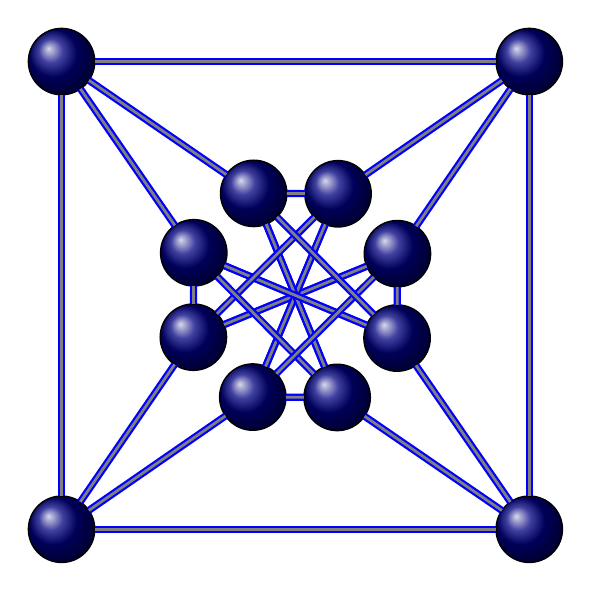
\begin{tikzpicture}[scale=.7]
       \GraphInit[vstyle=Shade]
       \SetVertexNoLabel
       \SetGraphShadeColor{blue!50!black}{blue}{gray} 
       \grChvatal[RA=6,RB=2]
    \end{tikzpicture}  
  \end{tkzexample}

\end{center}

\vfill\newpage
\subsection{\tkzname{Chvatal  graph II}}

\bigskip
\begin{center}
  \begin{tkzexample}[vbox]
    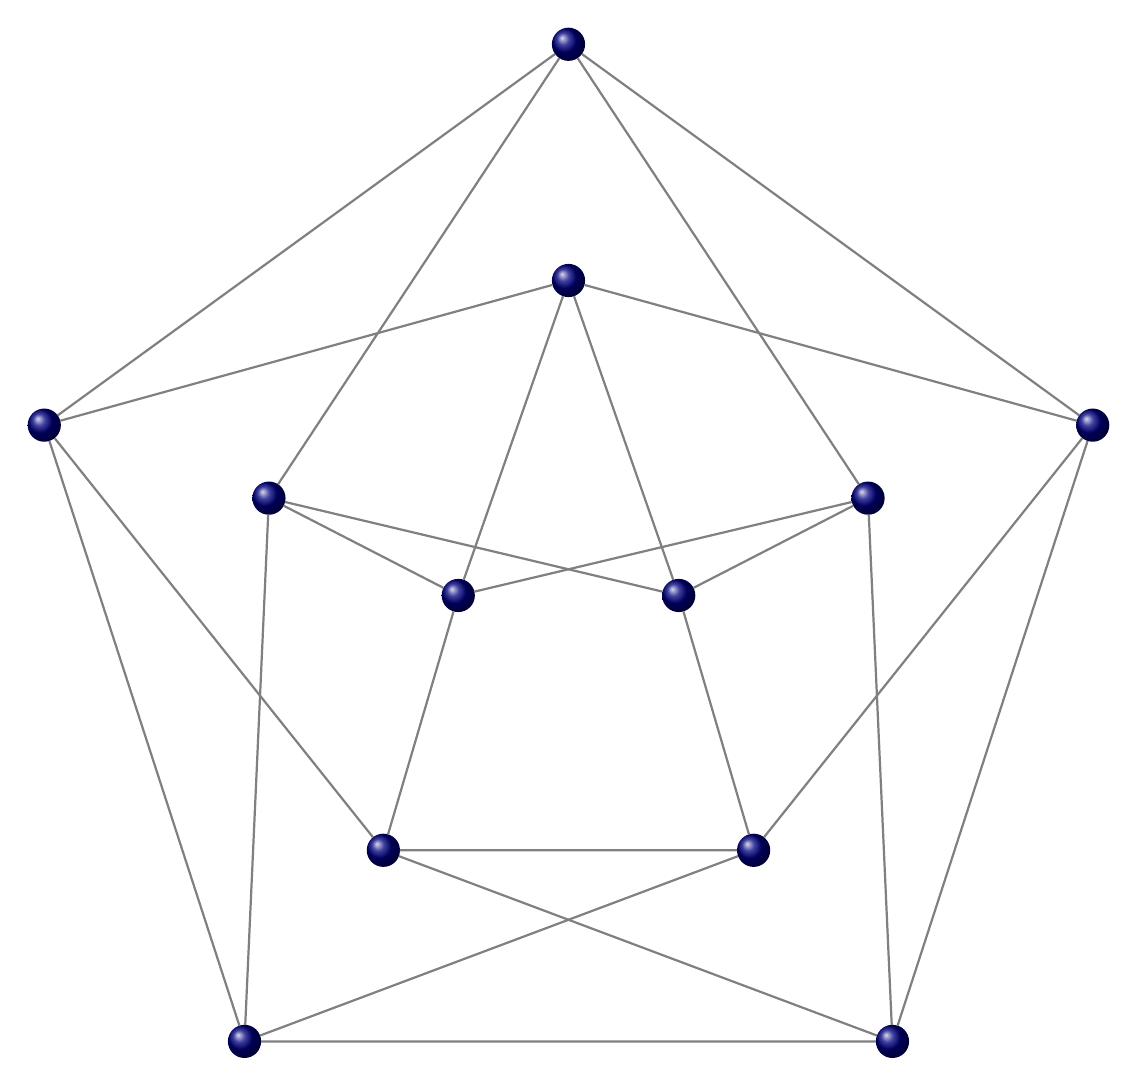
\begin{tikzpicture}
      \GraphInit[vstyle=Art]
      \SetGraphArtColor{blue!50!black}{gray}
      \grChvatal[form=2,RA=7,RB=4,RC=1.4] 
    \end{tikzpicture}
  \end{tkzexample}

\end{center}


\vfill\newpage
\subsection{\tkzname{Chvatal  graph III}}

\bigskip
\begin{center}
  \begin{tkzexample}[vbox]
    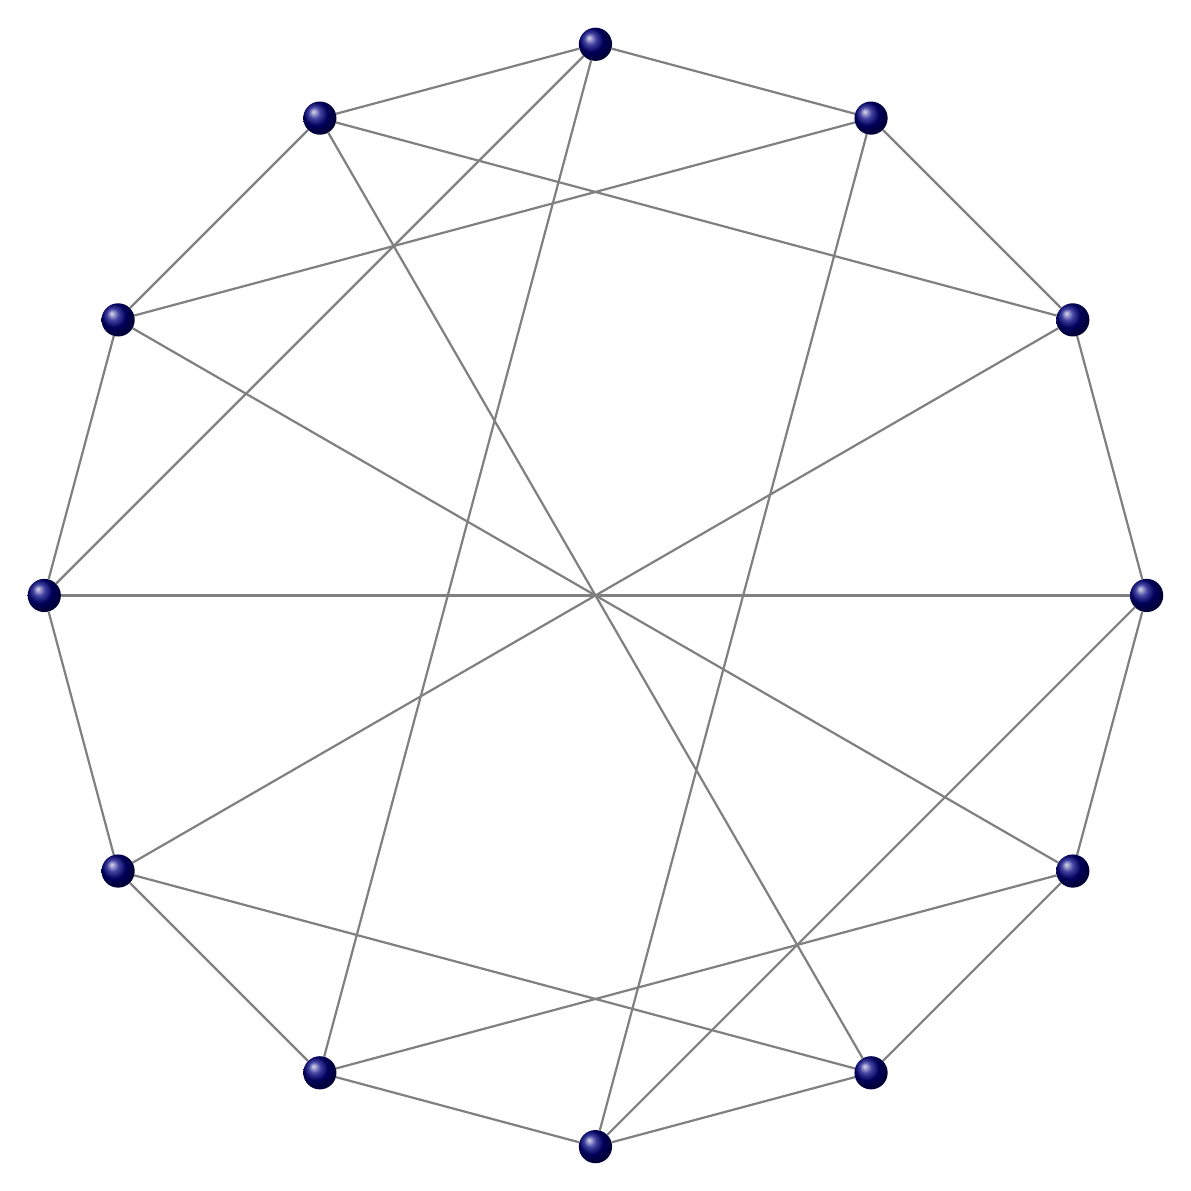
\begin{tikzpicture}
     \GraphInit[vstyle=Art]
     \SetGraphArtColor{blue!50!black}{gray}  
     \grChvatal[form=3,RA=7] 
    \end{tikzpicture}
  \end{tkzexample}

\end{center}

\endinput
\newpage\section{Crown}\label{crown}
%<––––––––––––––––––––––––––––––––––––––––––––––––––––––––––––––––––––––––––>
%<–––––––––––––––––––––––––––––    Crown    ––––––––––––––––––––––––––––––––>
%<––––––––––––––––––––––––––––––––––––––––––––––––––––––––––––––––––––––––––>
\begin{NewMacroBox}{grCrown}{\oarg{options}\var{integer}}


\medskip
From MathWord : \url{http://mathworld.wolfram.com/CrownGraph.html}  

\emph{The Crown graph  for an integer  is the graph with vertex set
$\{x_0,x_1,\dots,x_{n-1},y_0,y_1,\dots,y_{n-1}\}$\hfill\break
and edge set \hfill\break
$\{(x_i,x_j): 0\leq i,j\leq n-1,i \not=j\}$.}
\href{http://mathworld.wolfram.com/topics/GraphTheory.html}%
           {\textcolor{blue}{MathWorld}} by \href{http://en.wikipedia.org/wiki/Eric_W._Weisstein}%
           {\textcolor{blue}{E.Weisstein}}

\medskip
The Crown graph is implemented in \tkzname{tkz-berge} as \tkzcname{grCrown} with two forms.
\end{NewMacroBox}


\subsection{\tkzname{Crown graph form 1}}

\begin{center}
\begin{tkzexample}[vbox]
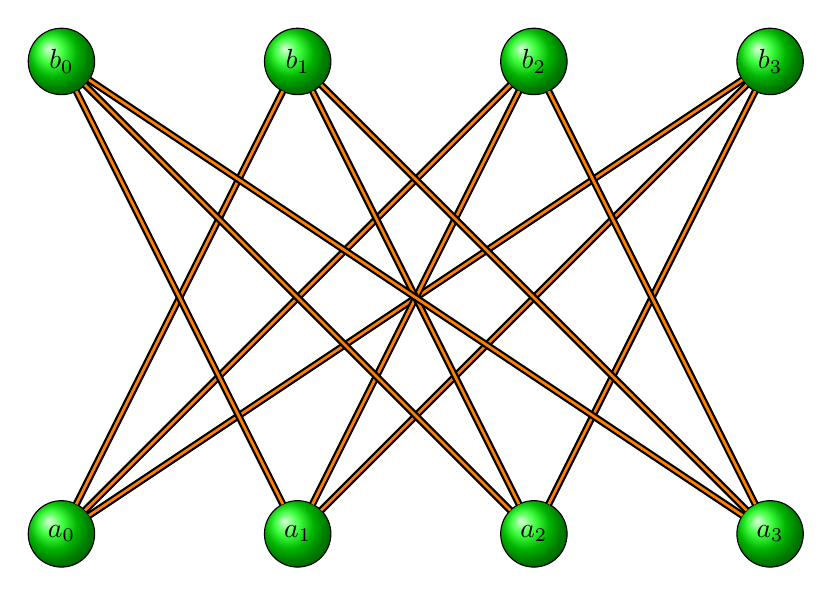
\begin{tikzpicture}
\tikzstyle{VertexStyle}   = [shape           = circle,
                             shading         = ball,
                             ball color      = green,
                             minimum size    = 24pt,
                             draw]
\tikzstyle{EdgeStyle}     = [thick,
                             double          = orange,
                             double distance = 1pt] 
\SetVertexLabel\SetVertexMath   
\grCrown[RA=3,RS=6]{4}
 \end{tikzpicture}
\end{tkzexample} 

\end{center}

\vfill\newpage
\subsection{\tkzname{Crown graph form 2}}

\begin{center}
\begin{tkzexample}[vbox]
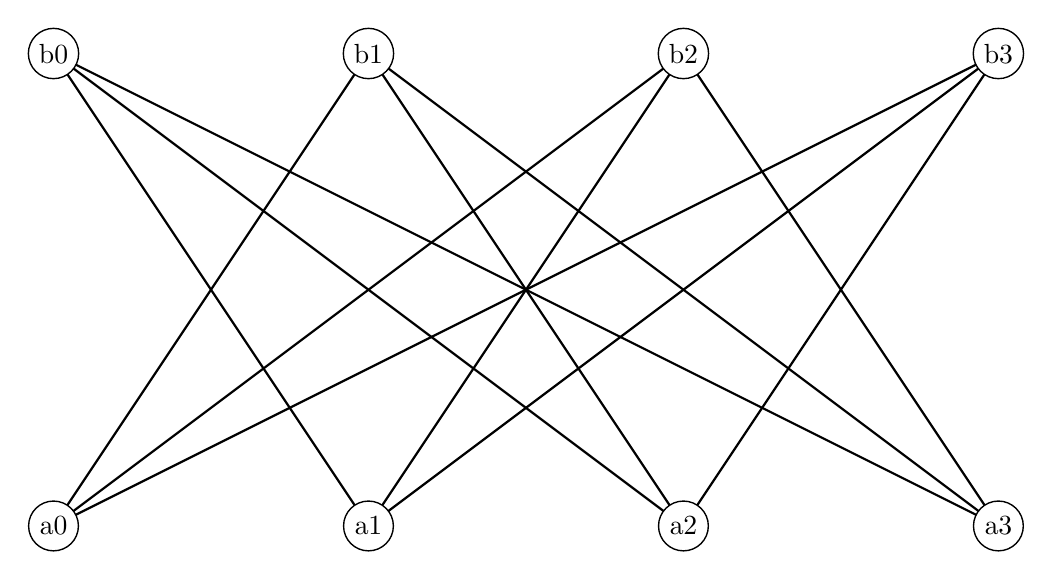
\begin{tikzpicture}
  \grCrown[form=2,RA=4,RS=6]{4}
 \end{tikzpicture}
\end{tkzexample} 
\end{center}

\endinput
\input{NamedGraphs-Cubicsymmetric.tex}
\newpage\section{Desargues}\label{desargues}
%<––––––––––––––––––––––––––––––––––––––––––––––––––––––––––––––––––––––––––>
%<–––––––––––––––––––––––––––––    Desargues –––––––––––––––––––––––––––––––>
%<––––––––––––––––––––––––––––––––––––––––––––––––––––––––––––––––––––––––––>
\begin{NewMacroBox}{grDesargues}{\oarg{options}}

\medskip
From Wikipedia : \url{http://en.wikipedia.org/wiki/Desargues_graph} 

\emph{ In the mathematical field of graph theory, the Desargues graph is a 3-regular graph with 20 vertices and 30 edges, formed as the Levi graph of the Desargues configuration.The Desargues graph can also be formed as a double cover of the Petersen graph, as the generalized Petersen graph G(10,3), or as the bipartite Kneser graph $H_{5,2}$.}

\medskip
From MathWord : \url{http://mathworld.wolfram.com/DesarguesGraph.html}  

\emph{ The Desargues graph is a cubic symmetric graph distance-regular graph on 20 vertices and 30 edges, illustrated above in several embeddings. It can be represented in LCF notation as  (Frucht 1976) and is isomorphic to the bipartite Kneser graph . It is the incidence graph of the Desargues configuration.}
\href{http://mathworld.wolfram.com/topics/GraphTheory.html}%
           {\textcolor{blue}{MathWorld}} by \href{http://en.wikipedia.org/wiki/Eric_W._Weisstein}%
           {\textcolor{blue}{E.Weisstein}}

\medskip
The Desargues graph is implemented in \tkzname{tkz-berge} as \tkzcname{grDesargues} with two forms.
\end{NewMacroBox}


\tikzstyle{VertexStyle} = [shape                = circle,%
                           color                = white,
                           fill                 = black,
                           very thin,
                           inner sep            = 0pt,%
                           minimum size         = 18pt,
                           draw]
\tikzstyle{EdgeStyle}   = [thick,%
                           double               = brown,%
                           double distance      = 1pt]
\SetVertexMath
\subsection{\tkzname{The Desargues graph : form 1}}
\begin{center}
\begin{tkzexample}[vbox]
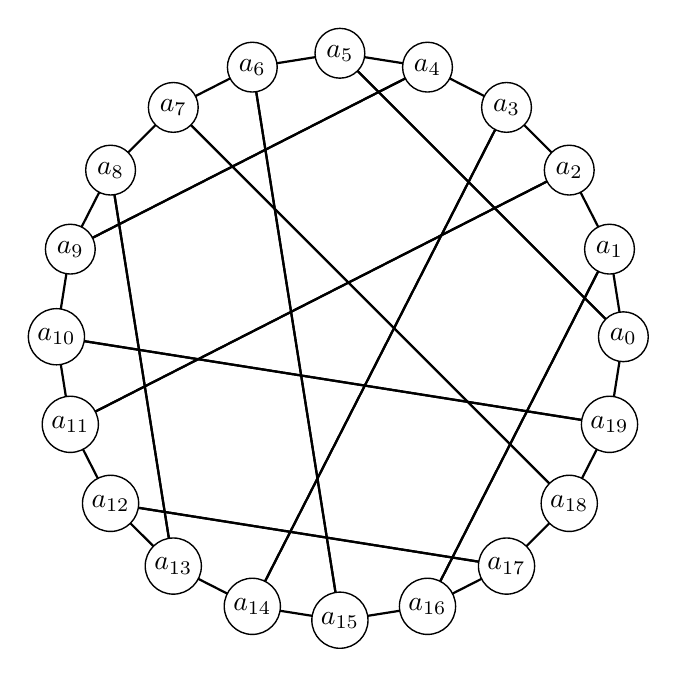
\begin{tikzpicture}[scale=.6]
    \grDesargues[Math,RA=6]
 \end{tikzpicture}
\end{tkzexample} 
\end{center}

\vfill\newpage
\subsection{\tkzname{The Desargues graph : form 2}}

\begin{center}
\begin{tkzexample}[vbox]
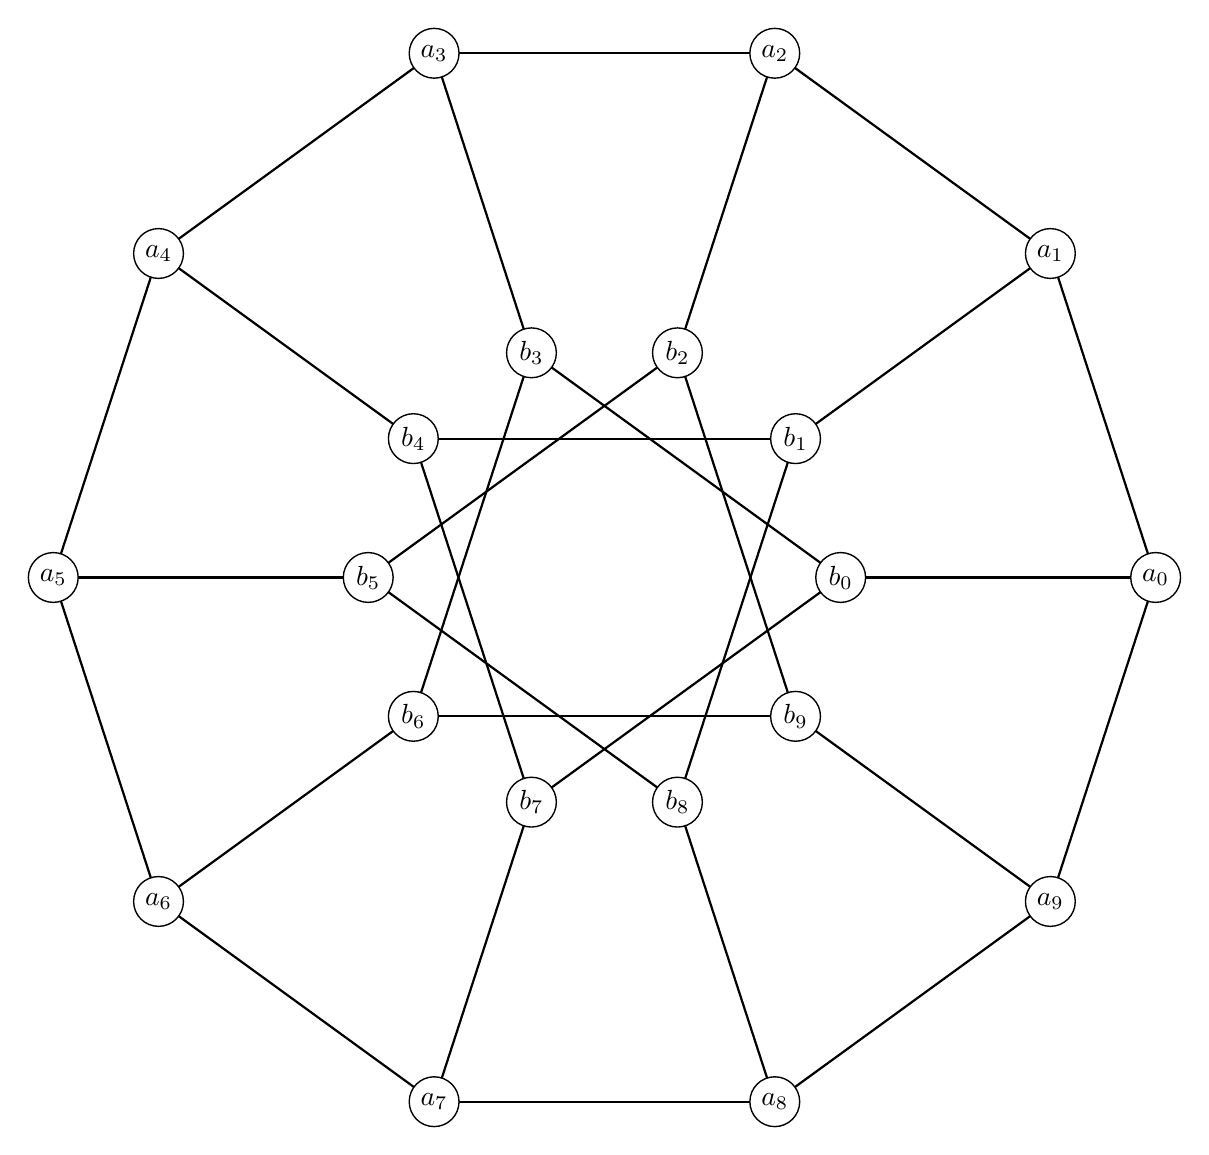
\begin{tikzpicture}
   \grDesargues[form=2,Math,RA=7]
 \end{tikzpicture}
\end{tkzexample} 
\end{center}

\vfill\newpage  
\subsection{The Desargues graph wth \tkzname{LCF notation}}

\begin{center}
\begin{tkzexample}[vbox]
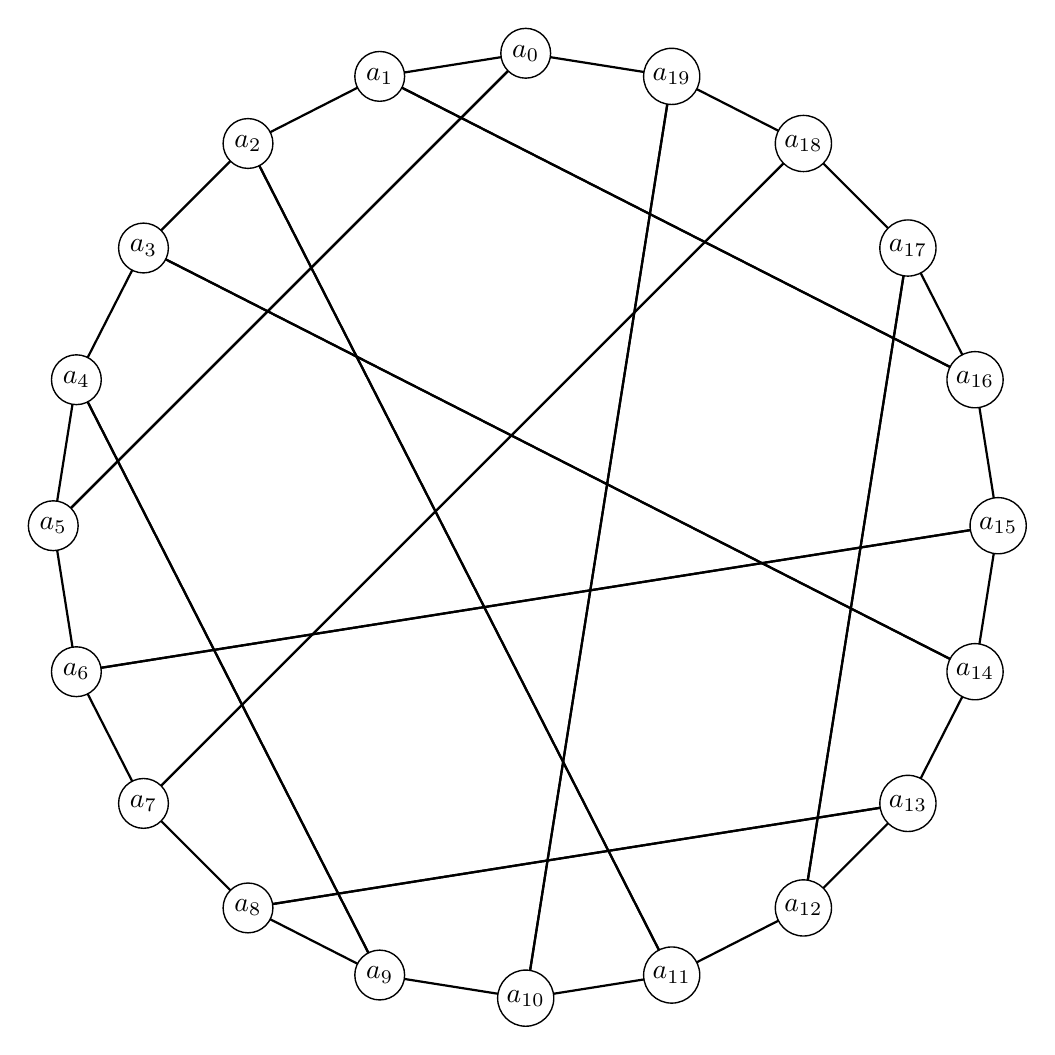
\begin{tikzpicture}[rotate=90]
   \grLCF[Math,RA=6]{5,-5,9,-9}{5}
 \end{tikzpicture}
\end{tkzexample} 
\end{center}


\vfill\newpage  
\subsection{The Desargues graph with \tkzcname{grGeneralizedPetersen}}
\begin{center}
\begin{tkzexample}[vbox]
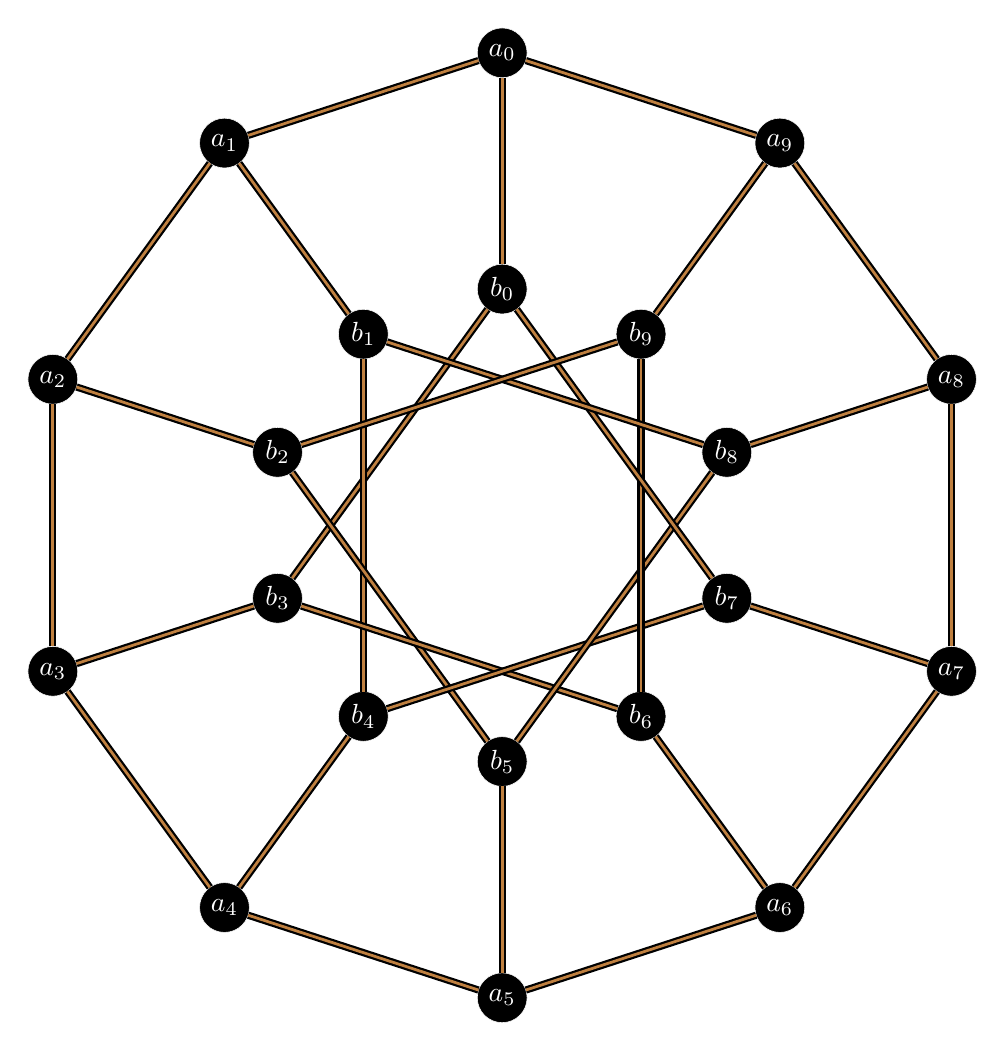
\begin{tikzpicture}[rotate=90]
  \tikzstyle{VertexStyle} = [shape                = circle,%
                             color                = white,
                             fill                 = black,
                             very thin,
                             inner sep            = 0pt,%
                             minimum size         = 18pt,
                             draw]
  \tikzstyle{EdgeStyle}    = [thick,%
                              double               = brown,%
                              double distance      = 1pt]  
  \grGeneralizedPetersen[Math,RA=6]{10}{3}
 \end{tikzpicture}
\end{tkzexample} 
\end{center}

\endinput
\newpage\section{Doyle}\label{doyle}
%<––––––––––––––––––––––––––––––––––––––––––––––––––––––––––––––––––––––––––>
%<–––––––––––––––––––––––––––––    Doyle  ––––––––––––––––––––––––––––––––>
%<––––––––––––––––––––––––––––––––––––––––––––––––––––––––––––––––––––––––––>
\begin{NewMacroBox}{grDoyle}{\oarg{options}}

\medskip
From MathWord : \url{http://mathworld.wolfram.com/DoyleGraph.html}  

\emph{The Doyle graph, sometimes also known as the Holt graph (Marušič et al. 2005), is the symmetric quartic graph on 27 nodes illustrated. It is a Symmetric Graph. Three embeddings are illustrated below.}
\href{http://mathworld.wolfram.com/topics/GraphTheory.html}%
           {\textcolor{blue}{MathWorld}} by \href{http://en.wikipedia.org/wiki/Eric_W._Weisstein}%
           {\textcolor{blue}{E.Weisstein}}

\medskip
The Doyle graph is implemented in \tkzname{tkz-berge} as \tkzcname{grDoyle} with three forms.
\end{NewMacroBox}

\subsection{\tkzname{The Doyle graph : form 1}}
\begin{center}
\begin{tkzexample}[vbox]
\begin{tikzpicture}[scale=.6] 
  \GraphInit[vstyle=Shade]
  \SetGraphShadeColor{red}{Maroon}{fondpaille}  
  \SetVertexNoLabel  
  \grDoyle[RA=7,RB=5,RC=3]
 \end{tikzpicture}
\end{tkzexample} 
\end{center}

\vfill\newpage
\subsection{\tkzname{The Doyle graph : form 2}}

\begin{center}
\begin{tkzexample}[vbox]
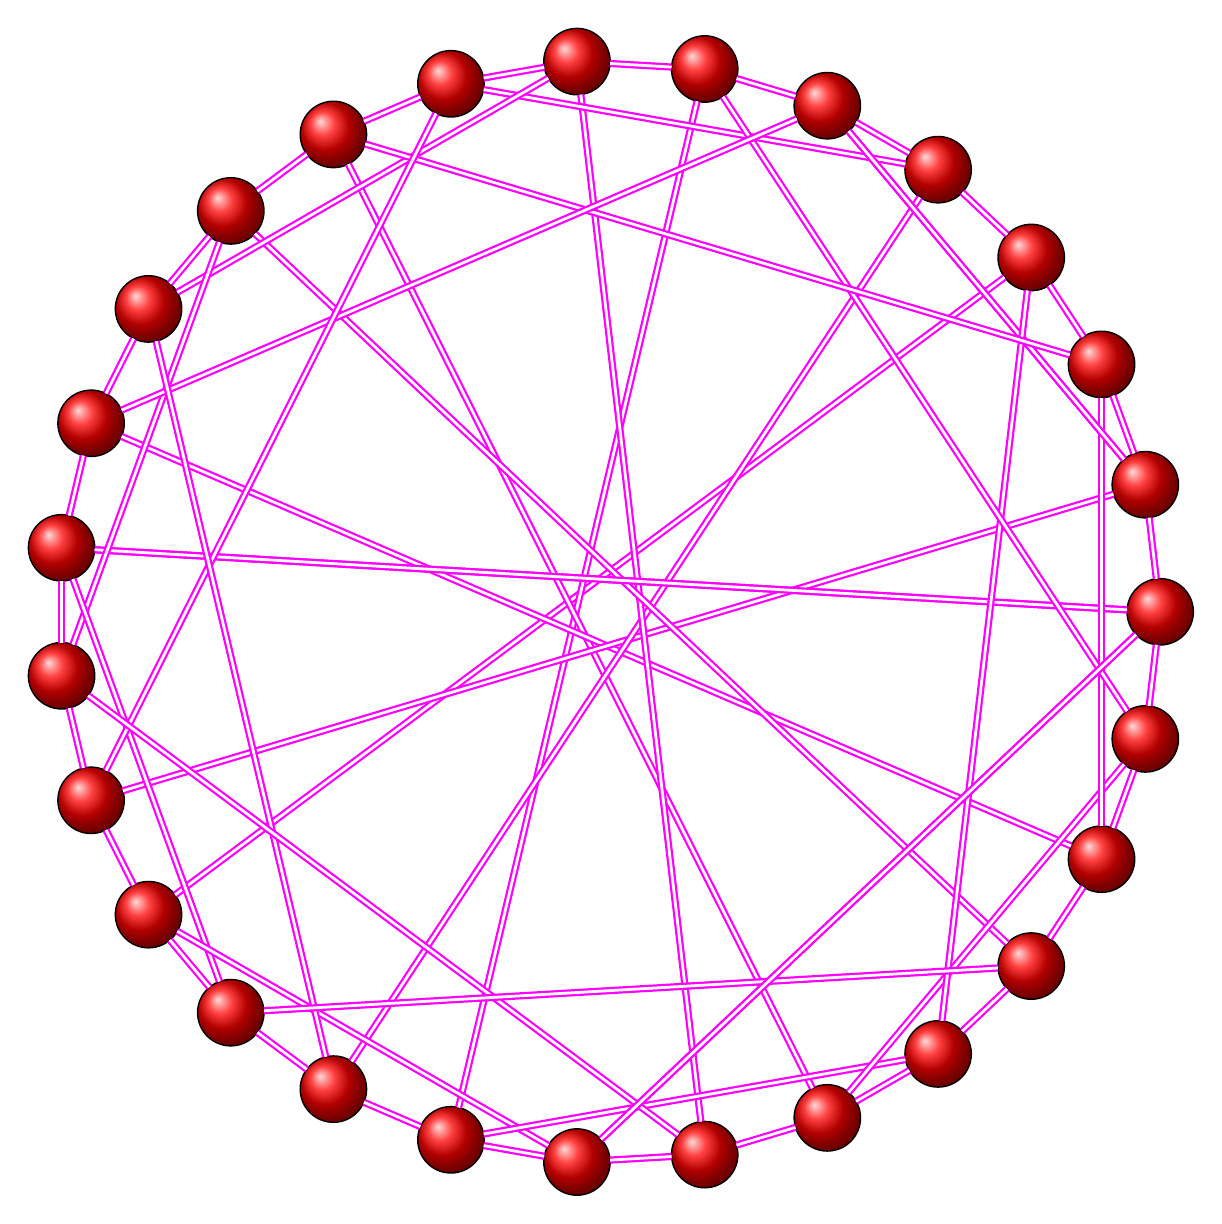
\begin{tikzpicture}
   \GraphInit[vstyle=Shade]
   \SetGraphShadeColor{red}{Magenta}{white} 
   \SetVertexNoLabel
   \grDoyle[form=2,RA=7]
 \end{tikzpicture}
\end{tkzexample} 
\end{center}

\vfill\newpage
\subsection{\tkzname{The Doyle graph : form 3}}
\begin{center}
 \begin{tkzexample}[vbox]
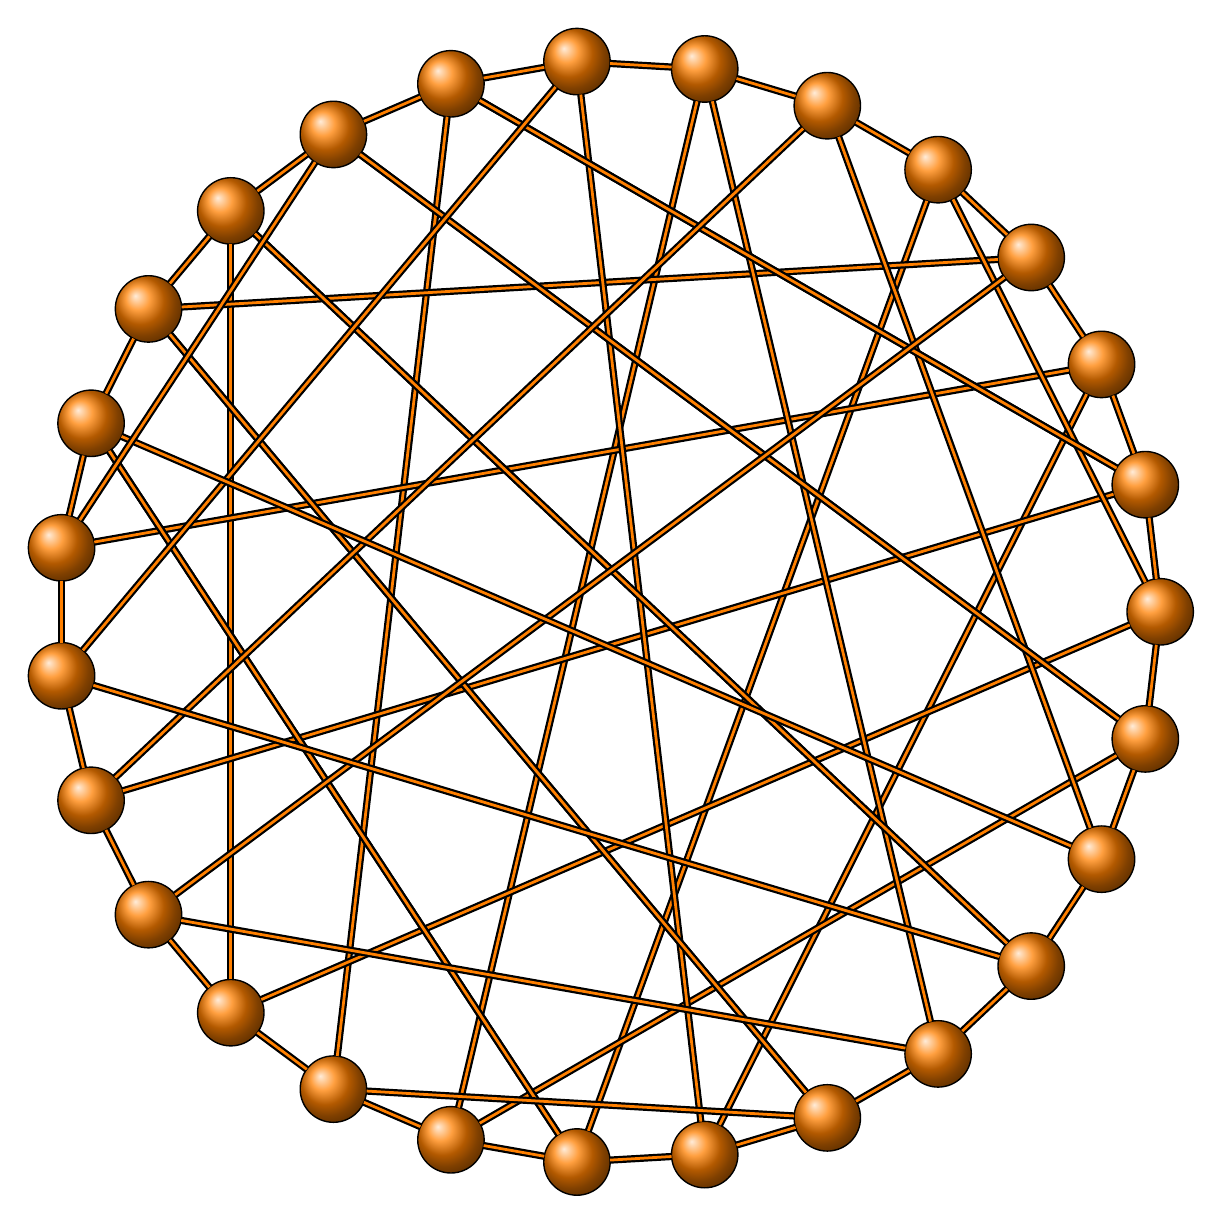
\begin{tikzpicture} 
  \SetGraphArtColor{red}{Magenta}{red}
   \GraphInit[vstyle=Shade]
   \SetVertexNoLabel 
   \grDoyle[form=3,RA=7,RB=2]
 \end{tikzpicture}
\end{tkzexample} 
\end{center}


\vfill\newpage

\subsection{27 nodes but not isomorphic to the Doyle graph}

\begin{center}
\begin{tkzexample}[vbox]
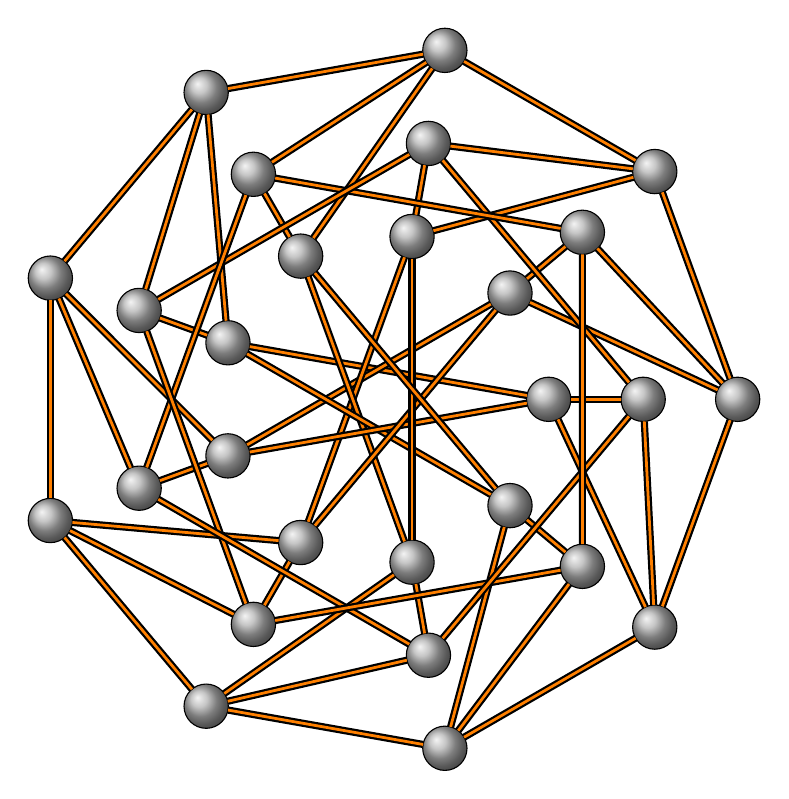
\begin{tikzpicture}[scale=.6] 
   \tikzstyle{VertexStyle} = [shape           = circle,
                              ball color      = gray!60,
                              minimum size    = 16pt,draw]
   \tikzstyle{EdgeStyle}   = [thick,color=black,%
                              double          = orange,%
                              double distance = 1pt] 
   \SetVertexNoLabel
   \grCycle[RA=7.5]{9}
   \grEmptyCycle[prefix=b,RA=5.5]{9}
   \grCirculant[prefix=c,RA=3.5]{9}{4}
   \EdgeIdentity{b}{c}{9}
   \EdgeMod{a}{c}{9}{1}
   \EdgeMod{a}{b}{9}{1}
   \EdgeInGraphMod{b}{9}{2}
   \end{tikzpicture}
\end{tkzexample} 
\end{center}


\endinput
\newpage\section{Folkman}\label{folkman}
%<––––––––––––––––––––––––––––––––––––––––––––––––––––––––––––––––––––––––––>
%<––––––––––––––––––––    Folkman            –––––––––––––––––––––––––––––––>
%<––––––––––––––––––––––––––––––––––––––––––––––––––––––––––––––––––––––––––>
\begin{NewMacroBox}{grFolkman}{\oarg{options}}

\medskip
From MathWorld : \url{http://mathworld.wolfram.com/FolkmanGraph.html}

\emph{The Folkman graph is a semisymmetric graph that has the minimum possible number of nodes 20.} 
\href{http://mathworld.wolfram.com/topics/GraphTheory.html}%
           {\textcolor{blue}{MathWorld}} by \href{http://en.wikipedia.org/wiki/Eric_W._Weisstein}%
           {\textcolor{blue}{E.Weisstein}}
\end{NewMacroBox}


\subsection{\tkzname{Folkman Graph LCF embedding}}
The code is

\begin{tkzexample}[code only]
\grLCF[RA=7]{5,-7,-7,5}{5}\end{tkzexample}

\begin{center}
\begin{tkzexample}[vbox]
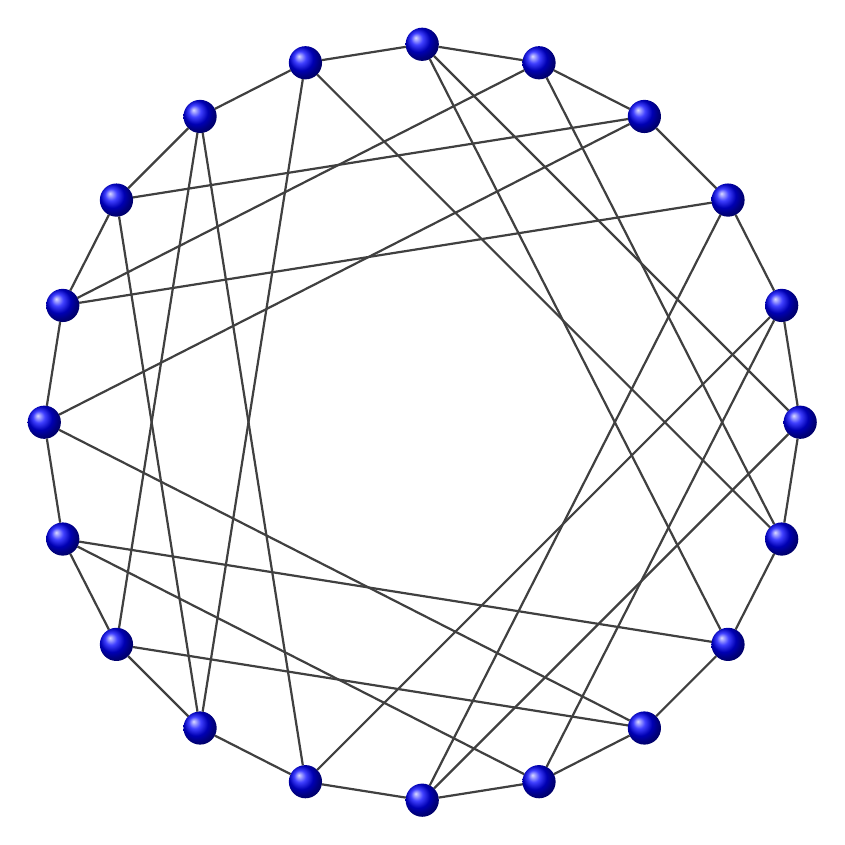
\begin{tikzpicture}[scale=.8]
      \GraphInit[vstyle=Art]
      \SetGraphArtColor{blue}{darkgray}
      \grFolkman[RA=6]
 \end{tikzpicture}
\end{tkzexample} 
\end{center}

\vfill\newpage


\subsection{\tkzname{Folkman Graph embedding 1}}
\begin{center}
\begin{tkzexample}[vbox]
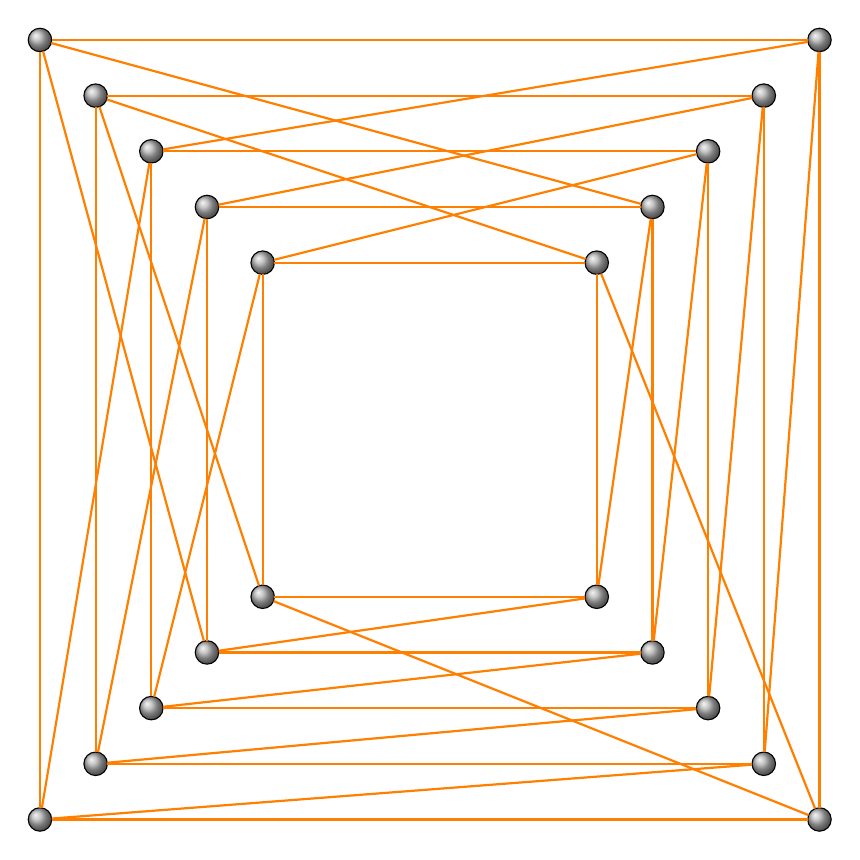
\begin{tikzpicture}[rotate=45]% 
     \tikzstyle{VertexStyle} = [shape           = circle,
                                shading         = ball,
                                ball color      = gray!60,
                                inner sep       = 3pt,
                                draw]
     \tikzstyle{EdgeStyle}  = [thick,orange]
     \SetVertexNoLabel 
     \grCycle[prefix=a,RA=3]{4}%
     \grCycle[prefix=b,RA=4]{4}%
     \grCycle[prefix=c,RA=5]{4}%
     \grCycle[prefix=d,RA=6]{4}%
     \grCycle[prefix=e,RA=7]{4}%
     \foreach \r/\s/\t in {a/d/e,b/e/a,c/a/b,d/b/c,e/c/d}{%
        \Edges(\r0,\s1,\r2,\t3,\r0)
        }
 \end{tikzpicture}
\end{tkzexample} 
\end{center}

\vfill\newpage

\subsection{\tkzname{Folkman Graph embedding 1 new code}}
{  \tikzstyle{VertexStyle} =[shape        = circle,%
                            shading       = ball,%
                            inner sep     = 4pt,%
                            draw]
  \tikzstyle{EdgeStyle}  = [thin,blue]

\begin{center}
\begin{tkzexample}[vbox]
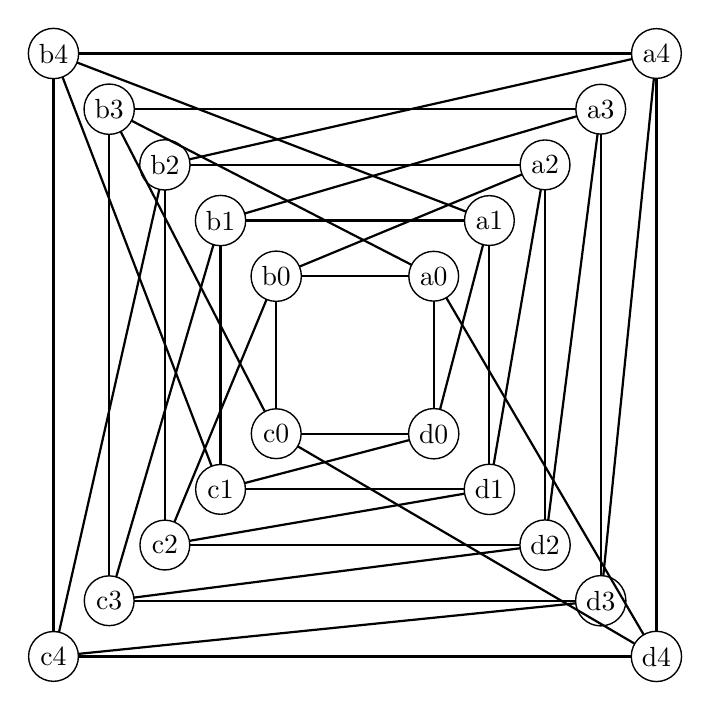
\begin{tikzpicture}
\begin{scope}[shift={(1,1)},rotate=45]\grEmptyPath[prefix=a,RA=1]{5}
  \end{scope}
\begin{scope}[shift={(-1,1)},rotate=135]\grEmptyPath[prefix=b,RA=1]{5}
  \end{scope}
\begin{scope}[shift={(-1,-1)},rotate=225]\grEmptyPath[prefix=c,RA=1]{5}
  \end{scope}
\begin{scope}[shift={(1,-1)},rotate=315]\grEmptyPath[prefix=d,RA=1]{5}
  \end{scope}
  \EdgeIdentity*{a}{b}{0,...,4}  \EdgeIdentity*{b}{c}{0,...,4}
  \EdgeIdentity*{c}{d}{0,...,4}  \EdgeIdentity*{d}{a}{0,...,4}
  \EdgeDoubleMod{a}{5}{0}{1}{b}{5}{3}{1}{1}
  \EdgeDoubleMod{a}{5}{2}{1}{b}{5}{0}{1}{2}
  \EdgeDoubleMod{a}{5}{1}{1}{d}{5}{0}{1}{3}
  \EdgeDoubleMod{c}{5}{2}{1}{b}{5}{0}{1}{2}
  \EdgeDoubleMod{c}{5}{0}{1}{b}{5}{3}{1}{1}
  \EdgeDoubleMod{c}{5}{1}{1}{d}{5}{0}{1}{3}
  \Edges(a0,d4,c0)
 \end{tikzpicture}
\end{tkzexample} 
\end{center}
}
\vfill\newpage

\subsection{\tkzname{Folkman Graph embedding 3}}

\begin{center}
\begin{tkzexample}[vbox]
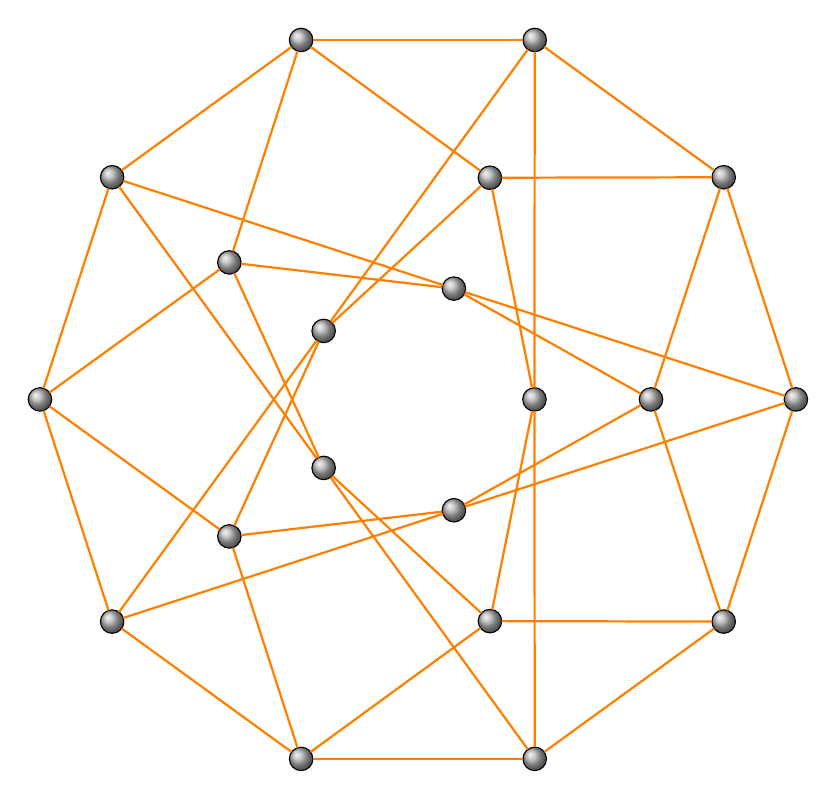
\begin{tikzpicture}[scale=.8]
   \SetVertexNoLabel
   \tikzstyle{VertexStyle} = [shape           = circle,
                              shading         = ball,
                              ball color      = gray!60,
                              inner sep       = 3pt,
                              draw]
   \tikzstyle{EdgeStyle}    = [thick,orange]  
   \grEmptyCycle[prefix=a,RA=1.85]{5} \grEmptyCycle[prefix=b,RA=3.7]{5}
   \grCycle[prefix=c,RA=6]{10}
   \EdgeDoubleMod{a}{5}{0}{1}{b}{5}{1}{1}{4}
   \EdgeDoubleMod{a}{5}{0}{1}{b}{5}{4}{1}{4}
   \EdgeDoubleMod{b}{5}{0}{1}{c}{10}{9}{2}{4}
   \EdgeDoubleMod{b}{5}{0}{1}{c}{10}{1}{2}{4}
   \EdgeDoubleMod{a}{5}{0}{1}{c}{10}{8}{2}{4}
   \EdgeDoubleMod{a}{5}{0}{1}{c}{10}{2}{2}{4}
\end{tikzpicture}
\end{tkzexample}
\end{center}

\endinput
\newpage\section{Foster}\label{foster}
%<––––––––––––––––––––––––––––––––––––––––––––––––––––––––––––––––––––––––––>
%<––––––––––––––––––––    Foster            –––––––––––––––––––––––––––––––>
%<––––––––––––––––––––––––––––––––––––––––––––––––––––––––––––––––––––––––––>

\begin{NewMacroBox}{grFoster}{\oarg{options}}

\medskip
From MathWord : \url{http://mathworld.wolfram.com/FosterGraph.html}

\emph{The Foster graph is a graph on 90 vertices and 135 arcs.  It has a unique order-15 LCF notations.}

\href{http://mathworld.wolfram.com/topics/GraphTheory.html}%
           {\textcolor{blue}{MathWorld}} by \href{http://en.wikipedia.org/wiki/Eric_W._Weisstein}%
           {\textcolor{blue}{E.Weisstein}} 
 \end{NewMacroBox}

\subsection{\tkzname{Foster graph}}

The macros is based on 

\begin{tkzexample}[code only]
\grLCF[Math,RA=7]{17, -9, 37, -37, 9, -17}{15}\end{tkzexample}

\vspace*{1cm}
\begin{center}
\begin{tkzexample}[vbox]
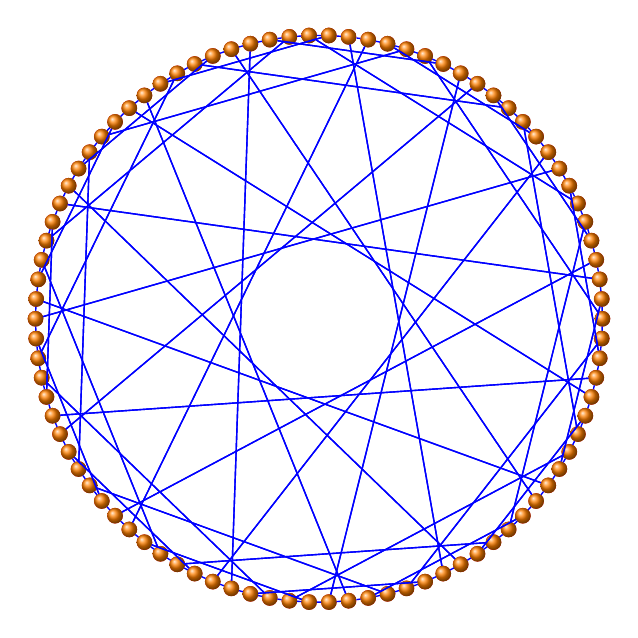
\begin{tikzpicture}[scale=.6]
  \renewcommand*{\VertexInnerSep}{2pt}
  \renewcommand*{\EdgeLineWidth}{0.5pt}
  \GraphInit[vstyle=Art] 
  \tikzset{VertexStyle/.append style={minimum size=2pt}} 
  \SetGraphColor{red}{blue}
  \grLCF[Math,RA=6]{17, -9, 37, -37, 9, -17}{15}
 \end{tikzpicture}
\end{tkzexample} 
\end{center}

\endinput

\newpage\section{Franklin}\label{franklin}
%<––––––––––––––––––––––––––––––––––––––––––––––––––––––––––––––––––––––––––>
%<–––––––––––––––––––––––––––––    Franklin  ––––––––––––––––––––––––––––––––>
%<––––––––––––––––––––––––––––––––––––––––––––––––––––––––––––––––––––––––––>
\begin{NewMacroBox}{grFranklin}{\oarg{options}}

\medskip
From MathWord : \url{http://mathworld.wolfram.com/FranklinGraph.html}  

\emph{The Franklin graph is the 12-vertex cubic graph shown above whose embedding on the Klein bottle divides it into regions having a minimal coloring using six colors, thus providing the sole counterexample to the Heawood conjecture.}
\href{http://mathworld.wolfram.com/topics/GraphTheory.html}%
           {\textcolor{blue}{MathWorld}} by \href{http://en.wikipedia.org/wiki/Eric_W._Weisstein}%
           {\textcolor{blue}{E.Weisstein}} 

\medskip
The Franklin graph is implemented in \tkzname{tkz-berge} as \tkzcname{grFranklin}.
\end{NewMacroBox}

\tikzstyle{VertexStyle} = [shape                =  circle,%
                           color                =  white,
                           fill                 =  black,
                           very thin,
                           inner sep            =  0pt,%
                           minimum size         =  18pt,
                           draw]
\tikzstyle{EdgeStyle}    = [thick,%
                            double               = brown,%
                            double distance      = 1pt]
\newcounter{tempi}\setcounter{tempi}{0}

\subsection{\tkzname{The Franklin graph : embedding 1}}
\begin{center}
\begin{tkzexample}[vbox]
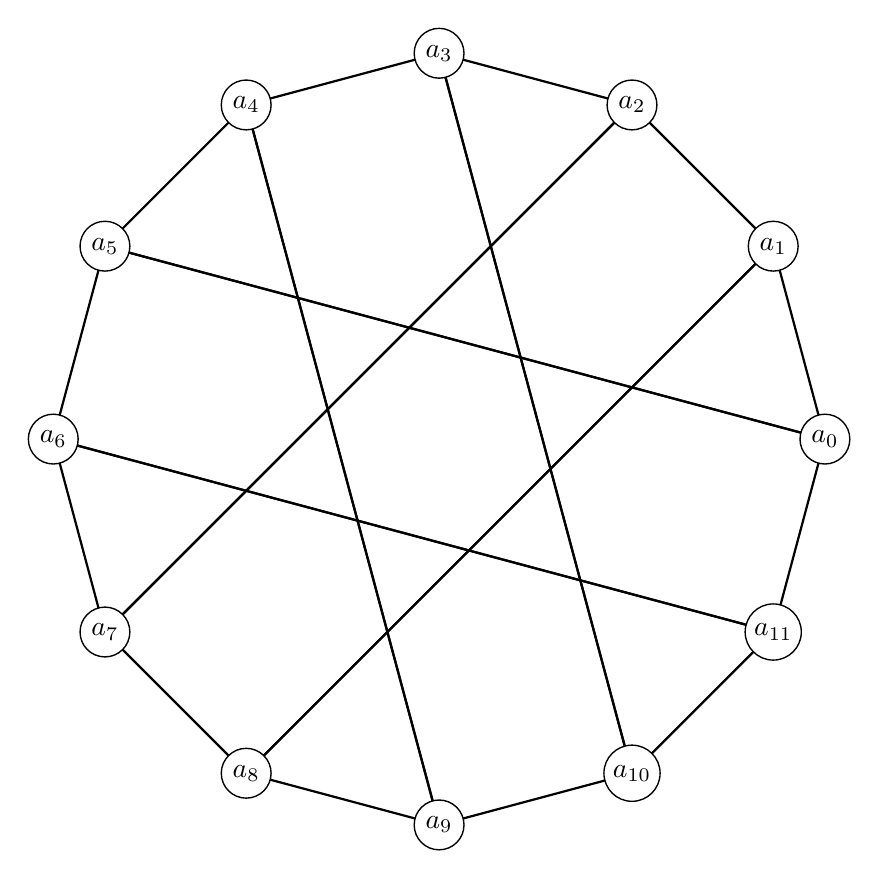
\begin{tikzpicture}[scale=.7]
   \grFranklin[Math,RA=7]
 \end{tikzpicture}
\end{tkzexample} 
\end{center}

\vfill\newpage
\subsection{\tkzname{The Franklin graph : embedding 2}}

\begin{center}
\begin{tkzexample}[vbox]
\begin{tikzpicture}
  \grCycle[Math,RA=4,prefix=a]{6}
  \grCycle[Math,RA=6,prefix=b]{6}
  \foreach \x in {0,...,5}{%
    \ifthenelse{\isodd{\x}}{%
     \pgfmathsetcounter{tempi}{\x-1}}{%
     \pgfmathsetcounter{tempi}{\x+1}}
     \Edge(a\x)(b\thetempi)
}
 \end{tikzpicture}
\end{tkzexample} 
\end{center}


\vfill\newpage
\subsection{\tkzname{The Franklin graph : with LCF notation embedding 3}}

\space*{2cm}
\begin{center}
\begin{tkzexample}[vbox]
\begin{tikzpicture}
   \grLCF[Math,RA=7]{-5,-3,3,5}{3}
 \end{tikzpicture}
\end{tkzexample} 
\end{center}

\endinput

\newpage\section{Gray}
%<––––––––––––––––––––––––––––––––––––––––––––––––––––––––––––––––––––––––––>
%<––––––––––––––––––––   Gray                –––––––––––––––––––––––––––––––>
%<––––––––––––––––––––––––––––––––––––––––––––––––––––––––––––––––––––––––––>
From MathWorld :\url{ http://mathworld.wolfram.com/GrayGraph.html}

\href{http://mathworld.wolfram.com/topics/GraphTheory.html}%
           {\textcolor{blue}{MathWorld}} by \href{http://en.wikipedia.org/wiki/Eric_W._Weisstein}%
           {\textcolor{blue}{E.Weisstein}} 
           
           
The Gray graph is a cubic semisymmetric graph on 54 vertices. It was discovered by Marion C. Gray in 1932, and was first published by Bouwer (1968). Malnic et al. (2004) showed that the Gray graph is indeed the smallest possible cubic semisymmetric graph.

It is the incidence graph of the Gray configuration.

The Gray graph has a single order-9 LCF Notation  and five distinct order-1 LCF notations.

The Gray graph has girth 8, graph diameter 6

It can be   represented in LCF notation as  $\big[-25,7,-7,13,-13,25\big]^9$ 

\begin{center}
\begin{tkzexample}[vbox]
\begin{tikzpicture}[rotate=90]
    \GraphInit[vstyle=Art]
    \SetGraphArtColor{gray}{red}
    \grLCF[Math,RA=6]{-25,7,-7,13,-13,25}{9}
 \end{tikzpicture}
\end{tkzexample} 
\end{center}

\endinput
\newpage\section{Groetzsch}
%<––––––––––––––––––––––––––––––––––––––––––––––––––––––––––––––––––––––––––>
%<––––––––––––––––––––   groetzsch            ––––––––––––––––––––––––––––––>
%<––––––––––––––––––––––––––––––––––––––––––––––––––––––––––––––––––––––––––>
\begin{NewMacroBox}{grGrotzsch}{\oarg{options}\var{$k$}}

\medskip
From  Wikipedia : \url{http://en.wikipedia.org/wiki/Grötzsch_graph}  

\emph{The Grötzsch graph is a triangle-free graph with 11 vertices, 20 edges, and chromatic number 4. It is named after German mathematician Herbert Grötzsch, and its existence demonstrates that the assumption of planarity is necessary in Grötzsch's theorem (Grötzsch 1959) that every triangle-free planar graph is 3-colorable.}

\medskip
From MathWord : \url{http://mathworld.wolfram.com/GroetzschGraph.html} 

\emph{The Grötzsch graph is smallest triangle-free graph with chromatic number four. It is identical to the Mycielski Graph of order four.}
\href{http://mathworld.wolfram.com/topics/GraphTheory.html}%
           {\textcolor{blue}{MathWorld}} by \href{http://en.wikipedia.org/wiki/Eric_W._Weisstein}%
           {\textcolor{blue}{E.Weisstein}} 

\end{NewMacroBox}


%GrotzschGraph
\tikzstyle{VertexStyle} = [shape           = circle,
                           shading         = ball,
                           ball color      = gray!60,
                           inner sep       = 3pt,
                           draw]
\SetVertexNoLabel
\tikzstyle{EdgeStyle}        = [thick,orange] 

\subsection{\tkzname{Grotzsch Graph : first form}}

\begin{center}
    \begin{tkzexample}[vbox]
  \begin{tikzpicture}
   \grGrotzsch[RA=3,RB=6]{6}%
 \end{tikzpicture}
\end{tkzexample} 
\end{center}


\vfill\newpage\null 
\subsection{\tkzname{Grotzsch Graph : second form}}
\SetVertexLabel
\begin{center}
\begin{tkzexample}[vbox]
\begin{tikzpicture}
   \grGrotzsch[form=2,RA=6,RB=3]{6}%
 \end{tikzpicture}
\end{tkzexample} 
\end{center}



\vfill\newpage\null
\subsection{\tkzname{Grotzsch Graph : third form}} 
From Wikipedia : \url{http://en.wikipedia.org/wiki/Complete_bipartite_graph} 

\tikzstyle{VertexStyle} = [shape           = circle,
                           shading         = ball,
                           ball color      = blue!60,
                           inner sep       = 6pt,
                           draw]
\SetVertexNoLabel
\tikzstyle{EdgeStyle}    = [thick,double= red,
                            double distance = 1pt] 

\begin{center}
  \begin{tkzexample}[vbox]
    \begin{tikzpicture}[rotate=-18]
     \draw[scale=.5,samples at={-6.4,-6.3,...,6.4},
                smooth,thick,
                variable=\t,
                double= red,
                double distance = 1pt]
           plot ({3*(1.5*cos(\t r) +3*cos(1.5*\t r))},%
                 {3*(1.5*sin(\t r) -3*sin(1.5*\t r))});
    \begin{scope}[rotate=36]
       \grStar[prefix=a,RA=2.2]{6}%
       \grEmptyCycle[prefix=b,RA=4.4]{5}%
    \end{scope}
    \end{tikzpicture}
  \end{tkzexample}

\end{center}

\endinput
\newpage\section{Heawood graph}\label{heawood}
%<––––––––––––––––––––––––––––––––––––––––––––––––––––––––––––––––––––––––––>
%<–––––––––––––––––––––––––––––    HEAWOOD  ––––––––––––––––––––––––––––––––>
%<––––––––––––––––––––––––––––––––––––––––––––––––––––––––––––––––––––––––––>
\begin{NewMacroBox}{grHeawood}{\oarg{options}}

\medskip
From Wikipedia \url{http://en.wikipedia.org/wiki/Heawood_graph}

\emph{The Heawood graph is an undirected graph with 14 vertices and 21 edges. Each vertex is adjacent to exactly three edges (that is, it is a cubic graph), and all cycles in the graph have six or more edges.  Percy John Heawood (1861-1955) was an English mathematician who spent a large amount of time on questions related to the four colour theorem.}

\medskip
From MathWorld \url{http://mathworld.wolfram.com/HeawoodGraph.html}

\emph{The Heawood graph is the unique $(3,6)$-cage graph and Moore graph and is  graph illustrated below in one of his embeddings.}
\href{http://mathworld.wolfram.com/topics/GraphTheory.html}%
           {\textcolor{blue}{MathWorld}} by \href{http://en.wikipedia.org/wiki/Eric_W._Weisstein}%
           {\textcolor{blue}{E.Weisstein}}
\end{NewMacroBox}

\subsection{\tkzname{Heawood graph}}
\begin{center}
\begin{tkzexample}[vbox]
\begin{tikzpicture}%
   \GraphInit[vstyle=Shade]
   \grHeawood[RA=7]
 \end{tikzpicture}
\end{tkzexample} 
\end{center}

\vfill\newpage
It can be represented in LCF notation as  $\big[5,-5\big]^7$

\tkzcname{grLCF[RA=5]\{5,9\}\{7\}} gives the result because  $-5 = 9\ mod\  14$.

\subsection{\tkzname{Heawood graph with LCF notation}}\label{lcf2}
\begin{center}
\begin{tkzexample}[vbox]
\begin{tikzpicture}%
   \GraphInit[vstyle=Art]
   \grLCF[RA=7]{5,9}{7}%
 \end{tikzpicture}
\end{tkzexample} 
\end{center}


\vfill\endinput
\newpage\section{Hypercube}
%<––––––––––––––––––––––––––––––––––––––––––––––––––––––––––––––––––––––––––>
%<––––––––––––––––––––  Hypercube            –––––––––––––––––––––––––––––––>
%<––––––––––––––––––––––––––––––––––––––––––––––––––––––––––––––––––––––––––>
From Wikipedia :\url{http://en.wikipedia.org/wiki/Hypercube_graph}

In the mathematical field of graph theory, the hypercube graph $Q_n$ is a  special regular graph with $2n$ vertices, which correspond to the subsets of a set with $n$ elements. Two vertices labelled by subsets S and T are joined by an edge if and only if S can be obtained from T by adding or removing a single element. Each vertex of $Q_n$ is incident to exactly $n$ edges (that is, $Q_n$ is $n$-regular), so the total number of edges is $2^{n-1}n$.
The name comes from the fact that the hypercube graph is the one-dimensional skeleton of the geometric hypercube.
Hypercube graphs should not be confused with cubic graphs, which are graphs that are 3-regular. The only hypercube that is a cubic graph is $Q_3$.

\tikzstyle{VertexStyle}       = [shape        = circle,%
                                 fill         = red,%
                                 inner sep    = 3pt,%
                                 outer sep    = 0pt,%
                                 draw]
\SetVertexNoLabel

\subsection{\tkzname{The hypercube graph $Q_4$} }

The code is on the next page.

\begin{center}
\begin{tkzexample}[vbox]
\begin{tikzpicture}
  \grCycle[RA=8]{8}
  \pgfmathparse{8*(1-4*sin(22.5)*sin(22.5))}
  \let\tkzbradius\pgfmathresult
  \grCirculant[prefix=b,RA=\tkzbradius]{8}{3}
  \makeatletter
  \foreach \vx in {0,...,7}{%
    \pgfmathsetcounter{tkz@gr@n}{mod(\vx+1,8)}
    \pgfmathsetcounter{tkz@gr@a}{mod(\vx+7,8)}
    \pgfmathsetcounter{tkz@gr@b}{mod(\thetkz@gr@n+1,8)}
    \Edge(a\thetkz@gr@n)(b\thetkz@gr@b)
    \Edge(b\thetkz@gr@a)(a\vx)
    }
  \makeatother
\end{tikzpicture}
\end{tkzexample}
\end{center}
\endinput
\newpage\section{The Seven Bridges of Königsberg}\label{seven}
%<––––––––––––––––––––––––––––––––––––––––––––––––––––––––––––––––––––––––––>
%<––––––––––––––––––         Königsberg       ––––––––––––––––––––––––––––––>
%<––––––––––––––––––––––––––––––––––––––––––––––––––––––––––––––––––––––––––>
\begin{NewMacroBox}{grKonisberg}{\oarg{options}\var{$k$}}

\medskip
From MathWorld : \url{http://mathworld.wolfram.com/KoenigsbergBridgeProblem.html}

\emph{The Königsberg bridge problem asks if the seven bridges of the city of Königsberg (left figure; Kraitchik 1942), formerly in Germany but now known as Kaliningrad and part of Russia, over the river Preger can all be traversed in a single trip without doubling back, with the additional requirement that the trip ends in the same place it began. This is equivalent to asking if the multigraph on four nodes and seven edges (right figure) has an Eulerian circuit. This problem was answered in the negative by Euler (1736), and represented the beginning of graph theory.}
\href{http://mathworld.wolfram.com/topics/GraphTheory.html}%
           {\textcolor{blue}{MathWorld}} by \href{http://en.wikipedia.org/wiki/Eric_W._Weisstein}%
           {\textcolor{blue}{E.Weisstein}} 

\medskip
From Wikipedia : \url{http://en.wikipedia.org/wiki/Seven_Bridges_of_Königsberg}

\emph{The paper written by Leonhard Euler on the Seven Bridges of Königsberg and published in 1736 is regarded as the first paper in the history of graph theory.\hfill\break
The Seven Bridges of Königsberg is a famous solved mathematics problem inspired by an actual place and situation. The city of Königsberg, Prussia (now Kaliningrad, Russia) is set on the Pregel River, and included two large islands which were connected to each other and the mainland by seven bridges. The problem is to decide whether it is possible to walk a route that crosses each bridge exactly once.\hfill\break
In 1736, Leonhard Euler proved that it was not possible. In proving the result, Euler formulated the problem in terms of graph theory, by abstracting the case of Königsberg — first, by eliminating all features except the landmasses and the bridges connecting them; second, by replacing each landmass with a dot, called a vertex or node, and each bridge with a line, called an edge or link. The resulting mathematical structure is called a graph.}
\end{NewMacroBox}

\subsection{\tkzname{Königsberg graph} with \tkzcname{grKonisberg}}
\begin{center}
\begin{tkzexample}[vbox]
 \begin{tikzpicture}[node distance=4cm]
  \grKonisberg
 \end{tikzpicture}
\end{tkzexample} 
\end{center}

\vfill\newpage
\subsection{\tkzcname{Königsberg graph} : fine embedding}
\begin{center}
\begin{tkzexample}[vbox]
 \begin{tikzpicture}
   \renewcommand*{\VertexBallColor}{orange!50!red} 
   \renewcommand*{\EdgeDoubleDistance}{2pt} 
   \SetGraphUnit{4}
   \GraphInit[vstyle=Shade]
   \tikzset{LabelStyle/.style =   {draw,
                                   fill  = yellow,
                                   text  = red}}
   \Vertex{A}
   \EA(A){B}
   \EA(B){C}
   {\SetGraphUnit{8} 
   \NO(B){D}}
   \Edge[label=1](B)(D)
   \tikzset{EdgeStyle/.append style = {bend left}}
   \Edge[label=4](A)(B)
   \Edge[label=5](B)(A)
   \Edge[label=6](B)(C)
   \Edge[label=7](C)(B)
   \Edge[label=2](A)(D)
   \Edge[label=3](D)(C)
 \end{tikzpicture}
\end{tkzexample} 
\end{center}

\endinput
\newpage\section{Levi Graph}\label{levi}
%<––––––––––––––––––––––––––––––––––––––––––––––––––––––––––––––––––––––––––>
%<––––––––––––––––––––      Levy             –––––––––––––––––––––––––––––––>
%<––––––––––––––––––––––––––––––––––––––––––––––––––––––––––––––––––––––––––>
\begin{NewMacroBox}{grLevi}{\oarg{options}}

\medskip

From Wikipedia \url{http://en.wikipedia.org/wiki/Levi_graph}

\emph{In combinatorics a Levi graph or incidence graph is a bipartite graph associated with an incidence structure. From a collection of points and lines in an incidence geometry or a projective configuration, we form a graph with one vertex per point, one vertex per line, and an edge for every incidence between a point and a line.\hfil\break 
In the mathematical field of graph theory, the Tutte–Coxeter graph or Tutte eight-cage is a 3-regular graph with 30 vertices and 45 edges. As the unique smallest cubic graph of girth 8 it is a cage and a Moore graph. It is bipartite, and can be constructed as the Levi graph of the generalized quadrangle. }

From MathWord : \url{http://mathworld.wolfram.com/LeviGraph.html} 

\emph{It has 30 nodes and 45 edges. It has girth 8, diameter 4, chromatic number 2. The Levi graph is a generalized polygon which is the point/line incidence graph of the generalized quadrangle . The graph  was first discovered by Tutte (1947), and is also called the Tutte-Coxeter graph , Tutte's cage  or "Tutte's (3,8)-cage".The Levi graph is the unique (3,8)-cage graph.\hfil\break
The incidence graph of a generic configuration is sometimes known as a Levi graph (Coxeter 1950).} 

\href{http://mathworld.wolfram.com/topics/GraphTheory.html}%
           {\textcolor{blue}{MathWorld}} by \href{http://en.wikipedia.org/wiki/Eric_W._Weisstein}%
           {\textcolor{blue}{E.Weisstein}}   
           
Some examples of Levi Graphs with this definition are~: 
\begin{itemize}
\item Desargues graph
\item Heawood graph
\item Heawood graph
\item Pappus graph
\item Gray graph 
\item Tutte eight-cage 
\end{itemize}

\end{NewMacroBox}

The two forms can be draw with :

 \begin{tkzexample}[code only]
   \grLevi[RA=7]\end{tkzexample}

and

 \begin{tkzexample}[code only]
    \grLevi[form=2,RA=7,RB=5,RC=3]\end{tkzexample}

You can see on the next pages, the two forms.
\vfill\newpage
Now I show you how to code this graph.

\subsection{\tkzname{Levy graph :form 1}}

\bigskip
\begin{center}
\begin{tkzexample}[vbox]
  \begin{tikzpicture}
    \GraphInit[vstyle=Art]
    \grLCF[prefix=a,RA=6]{-13,-9,7,-7,9,13}{5}
 \end{tikzpicture}
\end{tkzexample} 
\end{center}


\vfill\newpage

\subsection{\tkzname{Levy graph :form 2}}

\bigskip
\begin{center}
\begin{tkzexample}[vbox]
\begin{tikzpicture}
  \GraphInit[vstyle=Art]
  \grCycle[prefix=a,RA=7]{10}
  \EdgeInGraphMod{a}{10}{5}
  \grEmptyCycle[prefix=b,RA=5]{10}
  \grEmptyCycle[prefix=c,RA=3]{10}
  \EdgeInGraphMod{c}{10}{4}
 \end{tikzpicture}
\end{tkzexample} 
\end{center}
\endinput
\input{NamedGraphs-Mcgee.tex} 
\newpage\section{Möbius-Kantor Graph}\label{moebius}
%<––––––––––––––––––––––––––––––––––––––––––––––––––––––––––––––––––––––––––>
%<––––––––––––––––––––   Moebius             –––––––––––––––––––––––––––––––>
%<––––––––––––––––––––––––––––––––––––––––––––––––––––––––––––––––––––––––––>
\begin{NewMacroBox}{grMobiusKantor}{\oarg{options}}

\medskip
From MathWord : \url{http://mathworld.wolfram.com/Moebius-KantorGraph.html} 

\emph{The unique cubic symmetric graph on 16 nodes, illustrated above in several embeddings. It is 24 edges, girth 6, diameter 4, chromatic number 2, and is nonplanar but Hamiltonian. It can be represented in LCF notation  and is identical to a generalized Petersen graph .
} 

\href{http://mathworld.wolfram.com/topics/GraphTheory.html}%
           {\textcolor{blue}{MathWorld}} by \href{http://en.wikipedia.org/wiki/Eric_W._Weisstein}%
           {\textcolor{blue}{E.Weisstein}}   
\end{NewMacroBox}




\subsection{\tkzname{Möbius Graph : form I}}

\begin{center}
\begin{tkzexample}[vbox]
\begin{tikzpicture}
   \GraphInit[vstyle=Shade]
   \SetGraphArtColor{red}{olive} 
   \SetVertexNoLabel
   \grMobiusKantor[RA=7]
\end{tikzpicture} 
\end{tkzexample}
\end{center}
 
\vfill\newpage
\subsection{\tkzname{Möbius Graph : form II}}
 
\begin{center}
\begin{tkzexample}[vbox]
\begin{tikzpicture}[rotate=22.5]
   \GraphInit[vstyle=Shade]
  \SetGraphArtColor{red!50}{brown!50} 
   \SetVertexNoLabel
   \grMobiusKantor[form=2,RA=7,RB=3]
 \end{tikzpicture}
\end{tkzexample} 
\end{center} 

\vfill\newpage
 \subsection{\tkzname{Möbius Graph : form III}}
\begin{center}
\begin{tkzexample}[vbox]
\begin{tikzpicture}
   \GraphInit[vstyle=Shade]
   \SetVertexNoLabel
   \grMobiusKantor[form=3,RA=7,RB=2]
 \end{tikzpicture}
\end{tkzexample} 
\end{center}
 
\vfill\newpage
\subsection{\tkzname{Möbius Graph with LCF notation}} 

\begin{center}
\begin{tkzexample}[vbox]
\begin{tikzpicture}[rotate=90]
   \GraphInit[vstyle=Shade]
   \SetVertexNoLabel
 \grLCF[RA=7]{5,-5}{8}
 \end{tikzpicture}
\end{tkzexample} 
\end{center}

\vfill\newpage
\subsection{\tkzname{Möbius Graph with \tkzcname{grGeneralizedPetersen}} } 

\begin{center}
\begin{tkzexample}[vbox] 
\begin{tikzpicture}
   \GraphInit[vstyle=Shade]
   \SetVertexNoLabel  
  \grGeneralizedPetersen[RA=7,RB=4]{8}{3} 
 \end{tikzpicture}
\end{tkzexample} 
\end{center}  

\vfill\newpage
%<––––––––––––––––––––––––––––––––––––––––––––––––––––––––––––––––––––––––––>
%<––––––––––––––––––––   Moebius     Ladder   –––––––––––––––––––––––––––––––>
%<––––––––––––––––––––––––––––––––––––––––––––––––––––––––––––––––––––––––––>
A Möbius ladder of order $2n$ is a simple graph obtained by introducing a twist in a prism graph of order $2n$ that is isomorphic to the circulant graph  with order $2n$   and $L=\{1,n\}$

\url{http://mathworld.wolfram.com/MoebiusLadder.html}

\subsection{\tkzname{Möbius Ladder Graph}} 


\begin{center}
\begin{tkzexample}[vbox]
\begin{tikzpicture}
   \GraphInit[vstyle=Shade]
   \grMobiusLadder[RA=7,RB=2]{8}%
 \end{tikzpicture}
\end{tkzexample} 
\end{center} 


\vfill\newpage  
\subsection{\tkzname{Circulant Graph isomorphic to the last graph}}

\begin{center}
\begin{tkzexample}[vbox]
\begin{tikzpicture}
   \GraphInit[vstyle=Shade]
   \grCirculant[RA=7]{16}{1,8}%
\end{tikzpicture}  
\end{tkzexample}
\end{center} 

\endinput

\newpage\section{Möbius-Kantor Graph}\label{MK}
%<––––––––––––––––––––––––––––––––––––––––––––––––––––––––––––––––––––––––––>
%<––––––––––––––––––––––Möbius-Kantor Graph –––––––––––––––––––––––––––––––>
%<––––––––––––––––––––––––––––––––––––––––––––––––––––––––––––––––––––––––––>
\begin{NewMacroBox}{%
\newmacro{Möbius-Kantor Graph : \tkzcname{grMobiusKantor}}}{lightgray}
 \tkzcname{grMobiusKantor[|RA|=\meta{Number}]\var{Number}}

\medskip
From MathWord : \url{http://mathworld.wolfram.com/Moebius-KantorGraph.html}  

\emph{The unique cubic symmetric graph on 16 nodes, illustrated above in two embeddings. It is 24 edges, girth 6, diameter 4, chromatic number 2, and is nonplanar but Hamiltonian. It is identical to the generalized Petersen graph.}
\href{http://mathworld.wolfram.com/Moebius-KantorGraph.html}%
           {\textcolor{blue}{MathWorld}} by \href{http://en.wikipedia.org/wiki/Eric_W._Weisstein}%
           {\textcolor{blue}{E.Weisstein}}

\medskip
The Möbius-Kantor Graph is implemented in \tkzname{tkz-berge} as \tkzcname{grMobiusKantor}.
\end{NewMacroBox}

\subsection{Möbius-Kantor Graph with \tkzcname{grGeneralizedPetersen}}
\begin{center}
\begin{tkzexample}[vbox]
\begin{tikzpicture}
   \GraphInit[vstyle=Shade] 
   \SetVertexNoLabel
   \grGeneralizedPetersen[RA=7,RB=4]{3}{1}
 \end{tikzpicture}
\end{tkzexample} 
\end{center}

\vfill\newpage\null 


\subsection{\tkzname{MobiusKantor graph}}
\begin{center}
\begin{tkzexample}[vbox]
\begin{tikzpicture}
   \GraphInit[vstyle=Shade] 
   \SetVertexNoLabel
  \grMobiusKantor[RA=5]
 \end{tikzpicture}
\end{tkzexample} 
\end{center}


\endinput
\newpage\section{Pappus}
%<––––––––––––––––––––––––––––––––––––––––––––––––––––––––––––––––––––––––––>
%<–––––––––––––––––––––––––––––    Pappus   ––––––––––––––––––––––––––––––––>
%<––––––––––––––––––––––––––––––––––––––––––––––––––––––––––––––––––––––––––>
\begin{NewMacroBox}{grPappus}{\oarg{options}}

\medskip
From MathWord : \url{http://mathworld.wolfram.com/PappusGraph.html}

\emph{A cubic symmetric distance-regular graph on 18 vertices, illustrated below in three embeddings. It can be represented in LCF notation $[5,7,-7,7,-7,-5]^3$  (Frucht 1976).}
\href{http://mathworld.wolfram.com/topics/GraphTheory.html}%
           {\textcolor{blue}{MathWorld}} by \href{http://en.wikipedia.org/wiki/Eric_W._Weisstein}%
           {\textcolor{blue}{E.Weisstein}}   

From Wikipedia : \url{http://en.wikipedia.org/wiki/Pappus_graph}
\emph{In the mathematical field of graph theory, the Pappus graph is a 3-regular graph with 18 vertices and 27 edges, formed as the Levi graph of the Pappus configuration. It is a distance-regular graph, one of only 14 such cubic graphs according to Cubic symmetric graphs.}

This macro can be used with three different forms.
\end{NewMacroBox}

\bigskip


\subsection{\tkzname{Pappus Graph : form 1}} 
\begin{center}
\begin{tkzexample}[vbox]
\begin{tikzpicture}[scale=.7]
   \GraphInit[vstyle=Art]
   \grPappus[RA=7]
\end{tikzpicture} 
\end{tkzexample}  
\end{center}
 
\vfill\newpage     
\subsection{\tkzname{Pappus Graph : form 2}} 

\begin{center}
\begin{tkzexample}[vbox]
\begin{tikzpicture}
   \GraphInit[vstyle=Art]
   \SetGraphArtColor{red}{olive}
   \grPappus[form=2,RA=7,RB=5,RC=3]
 \end{tikzpicture}
\end{tkzexample} 
\end{center}

\vfill\newpage
\subsection{\tkzname{Pappus Graph : form 3}} 

\begin{center}
\begin{tkzexample}[vbox]
\begin{tikzpicture}
   \GraphInit[vstyle=Art]
   \SetGraphArtColor{gray}{blue}
   \grPappus[form=3,RA=7,RB=5,RC=2.5] 
 \end{tikzpicture}
\end{tkzexample} 
\end{center}


\endinput 
%!TEX root = /Users/ego/Boulot/TKZ/tkz-berge/NamedGraphs/doc/NamedGraphs-main.tex
\newpage\section{Petersen}\label{petersen} 
%<––––––––––––––––––––––––––––––––––––––––––––––––––––––––––––––––––––––––––>
%<––––––––––––––––––––    Petersen            –––––––––––––––––––––––––––––––>
%<––––––––––––––––––––––––––––––––––––––––––––––––––––––––––––––––––––––––––>
\begin{NewMacroBox}{grPetersen}{\oarg{options}}

\medskip
From MathWord : \url{http://mathworld.wolfram.com/PetersenGraph.html}

\emph{The Petersen graph is the graph , illustrated below in several embeddings, possessing 10 nodes, all of whose nodes have degree three. The Petersen graph is implemented in \tkzname{tkz-berge} as \tkzcname{grPetersen}.
The Petersen graph has girth 5, diameter 2, edge chromatic number 4, chromatic number 3.}

\href{http://mathworld.wolfram.com/topics/GraphTheory.html}%
           {\textcolor{blue}{MathWorld}} by \href{http://en.wikipedia.org/wiki/Eric_W._Weisstein}%
           {\textcolor{blue}{E.Weisstein}}   

From Wikipedia : \url{http://en.wikipedia.org/wiki/Petersen_graph}

\emph{In graph theory, the Petersen graph is an undirected graph with 10 vertices and 15 edges. It is a small graph that serves as a useful example and counterexample for many problems in graph theory. The Petersen graph is named for Julius Petersen, who in 1898 constructed it to be the smallest bridgeless cubic graph with no three-edge-coloring. Although the graph is generally credited to Petersen, it had in fact first appeared 12 years earlier, in 1886.}

This macro can be used with three different forms.
\end{NewMacroBox}

 \subsection{\tkzname{Petersen graph : form 1}}
\begin{center}
\begin{tkzexample}[latex=8cm]
\begin{tikzpicture}[scale=.8]
    \GraphInit[vstyle=Art]
    \SetGraphArtColor{red}{olive}
    \grPetersen[form=1,RA=5,RB=3]%
 \end{tikzpicture}
\end{tkzexample} 
\end{center}
\vfill\newpage
\subsection{\tkzname{Petersen graph : form 2}}

\bigskip
\begin{center}
\begin{tkzexample}[vbox]
\begin{tikzpicture}%
   \GraphInit[vstyle=Art]
   \SetGraphArtColor{red}{olive}
   \grPetersen[form=2,RA=7,RB=3]%
\end{tikzpicture}
\end{tkzexample}
\end{center}

\vfill\newpage
\subsection{\tkzname{Petersen graph : form 3}}

\bigskip
\begin{center}
\begin{tkzexample}[vbox]
\begin{tikzpicture}%
    \GraphInit[vstyle=Art]
    \SetGraphArtColor{red}{olive}
    \grPetersen[form=3,RA=7]%
\end{tikzpicture}
\end{tkzexample}
\end{center}

\vfill\newpage
\subsection{\tkzname{The line graph of the Petersen graph}}

\bigskip
\begin{center}
\begin{tkzexample}[vbox]
\begin{tikzpicture}
\GraphInit[vstyle=Art]\SetGraphArtColor{white}{blue}
  \begin{scope}[rotate=-90] \grCirculant[RA=1.5,prefix=a]{5}{2}\end{scope}
  \begin{scope}[rotate=-18] \grEmptyCycle[RA=4,prefix=b]{5}{2} \end{scope}
  \begin{scope}[rotate=18]  \grCycle[RA=7,prefix=c]{5}         \end{scope}
  \EdgeIdentity{a}{b}{5} 
  \EdgeIdentity{b}{c}{5}
  \EdgeDoubleMod{b}{5}{0}{1}{a}{5}{2}{1}{5}
  \EdgeDoubleMod{c}{5}{0}{1}{b}{5}{1}{1}{5}
 \end{tikzpicture}
\end{tkzexample} 
\end{center}

\vfill\newpage
%<––––––––––––––––––––––––––––––––––––––––––––––––––––––––––––––––––––––––––>
%<––––––––––––––––––––    Petersen   Gen     –––––––––––––––––––––––––––––––>
%<––––––––––––––––––––––––––––––––––––––––––––––––––––––––––––––––––––––––––>

\begin{NewMacroBox}{grGeneralizedPetersen}{\oarg{RA=\meta{Number},RB=\meta{Number}}\var{integer}\var{integer}}

\medskip
From MathWord : \url{http://mathworld.wolfram.com/GeneralizedPetersenGraph.html}

\emph{The generalized Petersen graph , also denoted $GP(n,k)$  , for $n \geq 3$ and $1\leq k \leq \lfloor (n-1)/2\rfloor $ is a graph consisting of an inner star polygon  (circulant graph ) and an outer regular polygon  (cycle graph ) with corresponding vertices in the inner and outer polygons connected with edges.  has  nodes and  edges. The Petersen graph is implemented in \tkzname{tkz-berge} as \tkzcname{grGeneralizedPetersen}.}
\href{http://mathworld.wolfram.com/GeneralizedPetersenGraph.html}%
           {\textcolor{blue}{MathWorld}} by \href{http://en.wikipedia.org/wiki/Eric_W._Weisstein}%
           {\textcolor{blue}{E.Weisstein}}

\medskip
From Wikipedia : \url{http://en.wikipedia.org/wiki/Petersen_graph}
\emph{In 1950 H. S. M. Coxeter introduced a family of graphs generalizing the Petersen graph. These graphs are now called generalized Petersen graphs, a name given to them in 1969 by Mark Watkins. In Watkins' notation, $G(n,k)$ is a graph with vertex set\hfill\break
 ${u_0, u_1,\dots, u_{n-1}, v_0, v_1, \dots, v_{n-1}}$\hfill\break
and edge set\hfill\break
${u_i u_{i+1}, u_i v_i, v_i u_{i+k}: i = 0,\dots,n-1}$\hfill\break
where subscripts are to be read modulo $n$ and $k<n/2$. Coxeter's notation for the same graph would be $\{n\}+\{n/k\}.$
The Petersen Graph itself is $G(5,2)$ or $\{5\}+\{5/2\}$.
}

This macro can be used with three different forms.
\end{NewMacroBox}

\subsection{\tkzname{Generalized Petersen graph} GP(5,1)}
\begin{center}
\begin{tkzexample}[vbox]
\begin{tikzpicture}[rotate=90,scale=.6]
  \GraphInit[vstyle=Art]\SetGraphArtColor{red}{olive}
  \renewcommand*{\VertexInnerSep}{4pt}
  \grGeneralizedPetersen[RA=5,RB=2]{5}{1}
 \end{tikzpicture}
\end{tkzexample} 
\end{center}

\vfill\newpage
\subsection{\tkzname{The Petersen graph} GP(5,2)}

\vspace*{2cm}
\begin{center}
\begin{tkzexample}[vbox]
\begin{tikzpicture}[rotate=90]
    \GraphInit[vstyle=Art]\SetGraphArtColor{red}{olive}
    \renewcommand*{\VertexInnerSep}{8pt}
    \grGeneralizedPetersen[RA=7,RB=4]{5}{2}
 \end{tikzpicture}
\end{tkzexample} 
\end{center}

\vfill\newpage
\subsection{\tkzname{Generalized Petersen graph} GP(6,2)}

\vspace*{2cm}\begin{center}
\begin{tkzexample}[vbox]
\begin{tikzpicture}[rotate=90]
  \GraphInit[vstyle=Art]\SetGraphArtColor{red}{olive}
  \renewcommand*{\VertexInnerSep}{8pt}
  \grGeneralizedPetersen[RA=7,RB=4]{6}{2}
 \end{tikzpicture}
\end{tkzexample} 
\end{center}

\vfill\newpage
\subsection{\tkzname{Generalized Petersen graph} GP(7,3)}

\vspace*{2cm}\begin{center}
\begin{tkzexample}[vbox]
\begin{tikzpicture}[rotate=90]
  \GraphInit[vstyle=Art]\SetGraphArtColor{red}{olive}
  \renewcommand*{\VertexInnerSep}{8pt}
  \grGeneralizedPetersen[RA=7,RB=4]{7}{3}
 \end{tikzpicture}
\end{tkzexample} 
\end{center}

\vfill\newpage
\subsection{\tkzname{Generalized Petersen graph} GP(11,5)}

\vspace*{2cm}\begin{center}
\begin{tkzexample}[vbox]
\begin{tikzpicture}[rotate=90]
  \renewcommand*{\VertexInnerSep}{8pt}
  \GraphInit[vstyle=Art]\SetGraphArtColor{red}{olive}
  \grGeneralizedPetersen[RA=7,RB=4]{11}{5}
 \end{tikzpicture}
\end{tkzexample} 
\end{center}


\endinput
 
%!TEX root = /Users/ego/Boulot/TKZ/tkz-berge/NamedGraphs/doc/NamedGraphs-main.tex
\newpage\section{ The five Platonics Graphs}
%<––––––––––––––––––––––––––––––––––––––––––––––––––––––––––––––––––––––––––>
%<––––––––––––––––––––  Platonic graphs      –––––––––––––––––––––––––––––––>
%<––––––––––––––––––––––––––––––––––––––––––––––––––––––––––––––––––––––––––>

The Platonic Graphs are the graphs formed by the edges and vertices of the five regular Platonic solids. The five Platonics Graphs  are illustrated below.  

\begin{enumerate}
  \item tetrahedral
  \item octahedral
  \item cube
  \item icosahedral
  \item dodecahedral
\end{enumerate} 


%<––––––––––––––––––––––––––––––––––––––––––––––––––––––––––––––––––––––––––>
%<––––––––––––––––––––––––––––––––––––––––––––––––––––––––––––––––––––––––––>
\begin{NewMacroBox}{grTetrahedral}{\oarg{RA=Number}}
From MathWord : \url{http://mathworld.wolfram.com/TetrahedralGraph.html} 

\emph{\tkzname{Tetrahedral Graph}  is the unique polyhedral graph on four nodes which is also the complete graph  and therefore also the wheel graph . It is implemented as \tkzcname{grTetrahedral}}
\href{http://mathworld.wolfram.com/TetrahedralGraph.html}%
           {\textcolor{blue}{MathWorld}} by \href{http://en.wikipedia.org/wiki/Eric_W._Weisstein}%
           {\textcolor{blue}{E.Weisstein}
}
It has :

\begin{enumerate}
 \item  4 nodes,
 \item  6 edges,
 \item  graph diameter 1.
\end{enumerate}

The  Tetrahedral Graph is 3-Regular
\end{NewMacroBox}

\subsection{\tkzname{Tetrahedral}}
\begin{center}
\begin{tkzexample}[vbox]
\begin{tikzpicture}[scale=.6]
      \GraphInit[vstyle=Shade]
      \renewcommand*{\VertexInnerSep}{4pt} 
      \SetVertexNoLabel\SetGraphShadeColor{red!50}{black}{red}
      \grTetrahedral[RA=5]
 \end{tikzpicture}
\end{tkzexample} 
\end{center}

\clearpage\newpage
\subsection{\tkzname{Tetrahedral LCF embedding}}

\vspace*{2cm}
\begin{center}
  \begin{tkzexample}[vbox]
\begin{tikzpicture}[rotate=18]
     \renewcommand*{\VertexInnerSep}{8pt} 
     \GraphInit[vstyle=Art]
     \SetGraphArtColor{red!50}{orange}
     \grLCF[RA=7]{2,-2}{2}
 \end{tikzpicture}
\end{tkzexample} 
\end{center}

\clearpage\newpage   
%<––––––––––––––––––––––––––––––––––––––––––––––––––––––––––––––––––––––––––>
%<––––––––––––––––––––––––––––––––––––––––––––––––––––––––––––––––––––––––––>

\begin{NewMacroBox}{grOctahedral}{\oarg{RA=\meta{Number},RB=\meta{Number}}}

\medskip
From MathWord : \url{http://mathworld.wolfram.com/OctahedralGraph.html} 

\emph{\tkzname{Octahedral Graph}  is isomorphic to the circulant graph $CI_{[1,2]}(6)$ . Two embeddings of this graph are illustrated below. It is implemented as \tkzcname{grOctahedral} or as \tkzcname{grSQCycle\{6\}}.}
\href{http://mathworld.wolfram.com/topics/GraphTheory.html}%
           {\textcolor{blue}{MathWorld}} by \href{http://en.wikipedia.org/wiki/Eric_W._Weisstein}%
           {\textcolor{blue}{E.Weisstein}}   

It has :

\begin{enumerate}
 \item  6 nodes,
 \item  12 edges,
 \item  graph diameter 2.
\end{enumerate}

\medskip
 The  Octahedral Graph is 4-Regular.
\end{NewMacroBox}


\medskip
\subsection{\tkzname{Octahedral}}
\begin{center}
\begin{tkzexample}[vbox]
\begin{tikzpicture}
  \grOctahedral[RA=6,RB=2]
 \end{tikzpicture}
\end{tkzexample} 
\end{center}

\vfill\newpage\null
\begin{center}
\begin{tkzexample}[vbox]
\begin{tikzpicture}
       \grSQCycle[RA=5]{6}
 \end{tikzpicture}
\end{tkzexample} 
\end{center}

\vfill\newpage\null
%<––––––––––––––––––––––––––––––––––––––––––––––––––––––––––––––––––––––––––>
%<––––––––––––––––––––––––––––––––––––––––––––––––––––––––––––––––––––––––––>

\medskip
\begin{NewMacroBox}{grCubicalGraph}{\oarg{RA=\meta{Number},RB=\meta{Number}}}

\medskip
From MathWord : \url{http://mathworld.wolfram.com/CubicalGraph.html} 

\emph{\tkzname{Cubical Graph}  is isomorphic to a generalized Petersen graph  $PG_{[4,1]}$, to a bipartite Kneser graph , to a crown graph and it is equivalent to the Cycle Ladder $CL(4)$. Two embeddings of this graph are illustrated below. It is implemented as \tkzcname{grCubicalGraph} or \tkzcname{grPrism\{4\}}.}
\href{http://mathworld.wolfram.com/CubicalGraph.html}%
           {\textcolor{blue}{MathWorld}} by \href{http://en.wikipedia.org/wiki/Eric_W._Weisstein}%
           {\textcolor{blue}{E.Weisstein}}

It has :

\begin{enumerate}
 \item  8 nodes,
 \item  12 edges,
 \item  graph diameter 3.
\end{enumerate}

 The  Cubical Graph is 3-Regular.
\end{NewMacroBox}

\subsection{\tkzname{Cubical Graph : form 1}}
\begin{center}
  \begin{tkzexample}[vbox]
\begin{tikzpicture}
  \grCubicalGraph[RA=5,RB=2]
 \end{tikzpicture}
\end{tkzexample} 
\end{center}

\vfill\newpage\null 
\subsection{\tkzname{Cubical Graph : form 2}}
\begin{center}
  \begin{tkzexample}[vbox]
\begin{tikzpicture}
  \grCubicalGraph[form=2,RA=7,RB=4]
 \end{tikzpicture}
\end{tkzexample} 
\end{center}

\vfill\newpage
\subsection{\tkzname{Cubical LCF embedding}}

\vspace*{2cm}
\begin{center}
\begin{tkzexample}[vbox]
\begin{tikzpicture}[rotate=18]
    \GraphInit[vstyle=Art]\renewcommand*{\VertexInnerSep}{8pt} 
    \SetGraphArtColor{red!50}{orange}
    \grLCF[RA=7]{3,-3}{4}
 \end{tikzpicture}
\end{tkzexample} 
\end{center}

\clearpage\newpage
%<––––––––––––––––––––––––––––––––––––––––––––––––––––––––––––––––––––––––––>

\begin{NewMacroBox}{grIcosahedral}{\oarg{RA=\meta{Number},RB=\meta{Number},RC=\meta{Number}}}

\medskip
From MathWord : \url{http://mathworld.wolfram.com/IcosahedralGraph.html} 

\emph{The \tkzname{Icosahedral Graph}  is the Platonic graph whose nodes have the connectivity of the icosahedron, illustrated above in a number of embeddings. The icosahedral graph has 12 vertices and 30 edges. Since the icosahedral graph is regular and Hamiltonian, it has a generalized LCF notation.}
\href{http://mathworld.wolfram.com/IcosahedralGraph.html}%
           {\textcolor{blue}{MathWorld}} by \href{http://en.wikipedia.org/wiki/Eric_W._Weisstein}%
           {\textcolor{blue}{E.Weisstein}}

\medskip
It has :

\begin{enumerate}
 \item  12 nodes,
 \item  30 edges,
 \item  graph diameter 3.
\end{enumerate}

\medskip
 The  Icosahedral Graph is 5-Regular.
\end{NewMacroBox}

\medskip

\subsection{\tkzname{Icosahedral forme 1 }}

\tikzstyle{EdgeStyle}= [thick,%
                        double          = orange,%
                        double distance = 1pt] 

\begin{center}
\begin{tkzexample}[vbox]
\begin{tikzpicture}[scale=.8]
 \GraphInit[vstyle=Art]\renewcommand*{\VertexInnerSep}{4pt} 
 \SetGraphArtColor{red}{orange}
 \grIcosahedral[RA=5,RB=1]
 \end{tikzpicture}
\end{tkzexample} 
\end{center}

\clearpage\newpage    

\subsection{\tkzname{Icosahedral forme 2 }}
\vspace*{2cm}
\begin{center}
\begin{tkzexample}[vbox]
\begin{tikzpicture}[rotate=-30]
   \GraphInit[vstyle=Art]  \renewcommand*{\VertexInnerSep}{8pt} 
   \SetGraphArtColor{red!50}{orange}
   \grIcosahedral[form=2,RA=8,RB=2,RC=.8]
 \end{tikzpicture}
\end{tkzexample} 
\end{center}

\vfill\newpage

\subsection{\tkzname{Icosahedral} \tkzname{RA=1} et \tkzname{RB=7}}
\begin{center}
\begin{tkzexample}[vbox]
 \begin{tikzpicture}
    \GraphInit[vstyle=Art]  \renewcommand*{\VertexInnerSep}{8pt} 
    \SetGraphArtColor{red!50}{orange}
    \grIcosahedral[RA=1,RB=7]
 \end{tikzpicture}
\end{tkzexample} 
\end{center}

\clearpage\newpage    
\subsection{\tkzname{Icosahedral LCF embedding 1}}

\vspace*{2cm}
\begin{center}
\begin{tkzexample}[vbox]
\begin{tikzpicture}[rotate=18]
    \GraphInit[vstyle=Art]  \renewcommand*{\VertexInnerSep}{8pt} 
    \SetGraphArtColor{red!50}{orange}
    \grLCF[RA=7]{-4,-3,4}{6}
 \end{tikzpicture}
\end{tkzexample} 
\end{center}

\clearpage\newpage    
\subsection{\tkzname{Icosahedral LCF embedding 2}}

\vspace*{2cm}
\begin{center}
\begin{tkzexample}[vbox]
\begin{tikzpicture}[rotate=18]
   \GraphInit[vstyle=Art]
   \SetGraphArtColor{red!50}{orange}
   \grLCF[RA=7]{-2,2,3}{6}
 \end{tikzpicture}
\end{tkzexample} 
\end{center}

\clearpage\newpage 
%<––––––––––––––––––––––––––––––––––––––––––––––––––––––––––––––––––––––––––>

\begin{NewMacroBox}{grDodecahedral}{\oarg{RA=\meta{Number},RB=\meta{Number},RC=\meta{Number},RD=\meta{Number}}}

\medskip
From MathWord : \url{http://mathworld.wolfram.com/DodecahedralGraph.html} 

\emph{The \tkzname{Icosahedral Graph}  is the Platonic graph corresponding to the connectivity of the vertices of a dodecahedron, illustrated above in four embeddings. The left embedding shows a stereographic projection of the dodecahedron, the second an orthographic projection, the third is from Read and Wilson, and the fourth is derived from LCF notation.}
\href{http://mathworld.wolfram.com/DodecahedralGraph.html}%
           {\textcolor{blue}{MathWorld}} by \href{http://en.wikipedia.org/wiki/Eric_W._Weisstein}%
           {\textcolor{blue}{E.Weisstein}}

\medskip
It has :

\begin{enumerate}
 \item  20 nodes,
 \item  30 edges,
 \item  graph diameter 5.
\end{enumerate}

\medskip
 The  Dodecahedral Graph is 3-Regular.
\end{NewMacroBox}

\medskip
\subsection{\tkzname{Dodecahedral}}

\begin{center}
\begin{tkzexample}[vbox]
\begin{tikzpicture}[rotate=18,scale=.6]
   \GraphInit[vstyle=Art]
   \SetGraphArtColor{red!50}{orange}
   \grDodecahedral[RA=7,RB=4,RC=2,RD=1]
 \end{tikzpicture}
\end{tkzexample} 
\end{center}

\subsection{\tkzname{Dodecahedral other embedding}}

\vspace*{2cm}
\begin{center}
\begin{tkzexample}[vbox]
\begin{tikzpicture}
   \grCycle[RA=7,prefix=a]{10}
   \grSQCycle[RA=4,prefix=b]{10}
     \foreach \v in {0,...,9}
       {\Edge(a\v)(b\v)}
 \end{tikzpicture}
\end{tkzexample} 
\end{center}

\vfill\newpage
\subsection{\tkzname{Dodecahedral LCF embedding}}

\vspace*{2cm}
\begin{center}
\begin{tkzexample}[vbox]
\begin{tikzpicture}[rotate=18]
   \GraphInit[vstyle=Art]
   \SetGraphArtColor{red!50}{orange}
   \grLCF[RA=7]{10,7,4,-4,-7,10,-4,7,-7,4}{2}
 \end{tikzpicture}
\end{tkzexample} 
\end{center}


\endinput
   
\newpage\section{Robertson}\label{robertson}
%<––––––––––––––––––––––––––––––––––––––––––––––––––––––––––––––––––––––––––>
%<––––––––––––––––––––    Robertson          –––––––––––––––––––––––––––––––>
%<––––––––––––––––––––––––––––––––––––––––––––––––––––––––––––––––––––––––––>
\begin{NewMacroBox}{grRobertson}{\oarg{options}\var{$k$}}

\medskip
From MathWord : \url{http://mathworld.wolfram.com/RobertsonGraph.html} 

\medskip
\emph{The Robertson graph is the unique (4,5)-cage graph, illustrated below. It has 19 vertices and 38 edges. It has girth 5, diameter 3, chromatic number 3, and is a quartic graph.} 
\href{http://mathworld.wolfram.com/topics/GraphTheory.html}%
           {\textcolor{blue}{MathWorld}} by \href{http://en.wikipedia.org/wiki/Eric_W._Weisstein}%
           {\textcolor{blue}{E.Weisstein}}   

\end{NewMacroBox}

\subsection{\tkzname{Robertson  graph with \tkzcname{grRobertson} }}

The cage 

\medskip
\begin{center}
\begin{tkzexample}[vbox]
\begin{tikzpicture}[scale=.6]
  \GraphInit[vstyle=Art]
  \SetGraphArtColor{black}{gray}
  \grRobertson[RA=7]
 \end{tikzpicture}
\end{tkzexample} 
\end{center}

\clearpage\newpage
\subsection{\tkzname{Fine embedding of the Robertson  graph from RV}}

\begin{center}
 \begin{tikzpicture}[scale=.8]
     \tikzstyle{TempEdgeStyle}= [thick,black,%
                               double               = gray,%
                               double distance      = 1.5pt]%
   \SetVertexNoLabel
   \renewcommand*{\VertexBigMinSize}{10pt}
   \GraphInit[vstyle=Shade]
   \SetVertexNoLabel
   \SetUpEdge[style  = {thick,%
                        double          = orange,%
                        double distance = 1pt}]
   \SetGraphShadeColor{gray}{black}{gray}
   \tikzstyle{EdgeStyle} = [TempEdgeStyle]
   \begin{scope}[rotate=-30]
     \grEmptyCycle[RA=5.4]{3}
   \end{scope}
   \tikzstyle{EdgeStyle}= [TempEdgeStyle,bend right=10]
   \grCycle[prefix=b,RA=4]{12}
   \tikzstyle{EdgeStyle}= [TempEdgeStyle]
   \grCirculant[prefix=c,RA=2]{4}{2}
   \tikzstyle{EdgeStyle}= [TempEdgeStyle,bend left]
   \EdgeDoubleMod{c}{4}{0}{1}%
                 {b}{12}{4}{3}{4}
    \tikzstyle{EdgeStyle}= [TempEdgeStyle,bend right]
    \EdgeDoubleMod{c}{4}{0}{1}
                  {b}{12}{8}{3}{4}
    \tikzstyle{EdgeStyle}= [TempEdgeStyle]
    \EdgeDoubleMod{a}{3}{0}{1}%
                  {b}{12}{11}{4}{3}
    \EdgeDoubleMod{c}{4}{0}{1}%
                  {b}{12}{0}{3}{4}
    \tikzstyle{EdgeStyle}= [TempEdgeStyle,bend left=60]
    \EdgeDoubleMod{a}{3}{0}{1}%
                  {b}{12}{8}{4}{3}
    \tikzstyle{EdgeStyle}= [TempEdgeStyle,bend right=60]
    \EdgeDoubleMod{a}{3}{0}{1}%
                  {b}{12}{2}{4}{3}
    \tikzstyle{EdgeStyle}=[TempEdgeStyle,in=-50,out=-120,
                           relative,looseness=2.5]
    \EdgeDoubleMod{a}{3}{0}{1}%
                   {b}{12}{5}{4}{3}
   \end{tikzpicture}
\end{center}

\clearpage\newpage
Code for the Robertson Graph

\medskip
\begin{tkzexample}[code only]
\begin{tikzpicture}[scale=.9]
  \tikzstyle{TempEdgeStyle}= [thick,black,%
                              double               = gray,%
                              double distance      = 1.5pt]%
   \SetVertexNoLabel
   \renewcommand*{\VertexBigMinSize}{14pt}
   \GraphInit[vstyle=Shade]
   \SetVertexNoLabel
   \SetUpEdge[style  = {thick,%
                        double          = orange,%
                        double distance = 1pt}]

   \SetGraphShadeColor{gray}{black}{gray}
   \tikzstyle{EdgeStyle} = [TempEdgeStyle]
   \begin{scope}[rotate=-30]
     \grEmptyCycle[RA=5.4]{3}
   \end{scope}
   \tikzstyle{EdgeStyle}= [TempEdgeStyle,bend right=10]
   \grCycle[prefix=b,RA=4]{12}
   \tikzstyle{EdgeStyle}= [TempEdgeStyle]
   \grCirculant[prefix=c,RA=2]{4}{2}
   \tikzstyle{EdgeStyle}= [TempEdgeStyle,bend left]
   \EdgeDoubleMod{c}{4}{0}{1}%
                 {b}{12}{4}{3}{4}
    \tikzstyle{EdgeStyle}= [TempEdgeStyle,bend right]
    \EdgeDoubleMod{c}{4}{0}{1}
                  {b}{12}{8}{3}{4}
    \tikzstyle{EdgeStyle}= [TempEdgeStyle]
    \EdgeDoubleMod{a}{3}{0}{1}%
                  {b}{12}{11}{4}{3}
    \EdgeDoubleMod{c}{4}{0}{1}%
                  {b}{12}{0}{3}{4}
    \tikzstyle{EdgeStyle}= [TempEdgeStyle,bend left=60]
    \EdgeDoubleMod{a}{3}{0}{1}%
                  {b}{12}{8}{4}{3}
    \tikzstyle{EdgeStyle}= [TempEdgeStyle,bend right=60]
    \EdgeDoubleMod{a}{3}{0}{1}%
                  {b}{12}{2}{4}{3}
    \tikzstyle{EdgeStyle}=[TempEdgeStyle,in=-50,out=-120,
                           relative,looseness=2.5]
    \EdgeDoubleMod{a}{3}{0}{1}%
                   {b}{12}{5}{4}{3}
 \end{tikzpicture}
\end{tkzexample}  

\clearpage\newpage   
\subsection{\tkzname{Robertson  graph with new styles}}

The code  with new styles, the result is on the next page.

\bigskip
\begin{tkzexample}[code only]
  \begin{tikzpicture}[scale=1]
  \GraphInit[vstyle=Art]
  \SetGraphArtColor{gray}{red}
  \begin{scope}[rotate=-30]
    \grEmptyCycle[RA=5]{3}
  \end{scope}
  {\tikzset{EdgeStyle/.append style = {bend right=10}}
  \grCycle[prefix=b,RA=3.5]{12}}
  \grCirculant[prefix=c,RA=2]{4}{2}
  {\tikzset{EdgeStyle/.append style = {bend left}}
  \EdgeDoubleMod{c}{4}{0}{1}%
                {b}{12}{4}{3}{4}}
  {\tikzset{EdgeStyle/.append style = {bend right}}
   \EdgeDoubleMod{c}{4}{0}{1}
                 {b}{12}{8}{3}{4}}
   \EdgeDoubleMod{a}{3}{0}{1}%
                 {b}{12}{11}{4}{3}
   \EdgeDoubleMod{c}{4}{0}{1}%
                 {b}{12}{0}{3}{4}
  {\tikzset{EdgeStyle/.append style = {bend left=60}}
   \EdgeDoubleMod{a}{3}{0}{1}%
                 {b}{12}{8}{4}{3}}
  {\tikzset{EdgeStyle/.append style = {bend right=60}}
   \EdgeDoubleMod{a}{3}{0}{1}%
                 {b}{12}{2}{4}{3}}
   {\tikzset{EdgeStyle/.append style = {in=-50,out=-120,%
                                        relative,looseness=2.5}}
   \EdgeDoubleMod{a}{3}{0}{1}%
                  {b}{12}{5}{4}{3}}
 \end{tikzpicture}
\end{tkzexample} 

\begin{center}
\begin{tikzpicture}[scale=1]
\GraphInit[vstyle=Art]
\SetGraphArtColor{gray}{red}
\begin{scope}[rotate=-30]
  \grEmptyCycle[RA=5]{3}
\end{scope}
{\tikzset{EdgeStyle/.append style = {bend right=10}}
\grCycle[prefix=b,RA=3.5]{12}}
\grCirculant[prefix=c,RA=2]{4}{2}
{\tikzset{EdgeStyle/.append style = {bend left}}
\EdgeDoubleMod{c}{4}{0}{1}%
              {b}{12}{4}{3}{4}}
{\tikzset{EdgeStyle/.append style = {bend right}}
 \EdgeDoubleMod{c}{4}{0}{1}
               {b}{12}{8}{3}{4}}
 \EdgeDoubleMod{a}{3}{0}{1}%
               {b}{12}{11}{4}{3}
 \EdgeDoubleMod{c}{4}{0}{1}%
               {b}{12}{0}{3}{4}
{\tikzset{EdgeStyle/.append style = {bend left=60}}
 \EdgeDoubleMod{a}{3}{0}{1}%
               {b}{12}{8}{4}{3}}
{\tikzset{EdgeStyle/.append style = {bend right=60}}
 \EdgeDoubleMod{a}{3}{0}{1}%
               {b}{12}{2}{4}{3}}
 {\tikzset{EdgeStyle/.append style = {in=-50,out=-120,%
                                      relative,looseness=2.5}}
 \EdgeDoubleMod{a}{3}{0}{1}%
                {b}{12}{5}{4}{3}}
\end{tikzpicture} 
\end{center} 
\clearpage\newpage
%<––––––––––––––––––––––––––––––––––––––––––––––––––––––––––––––––––––––––––>
%<––––––––––––––––––––    Robertson  Wegner  –––––––––––––––––––––––––––––––>
%<––––––––––––––––––––––––––––––––––––––––––––––––––––––––––––––––––––––––––>
\begin{NewMacroBox}{grRobertsonWegner}{\oarg{options}\var{$k$}}

\medskip
From MathWord : \url{http://mathworld.wolfram.com/Robertson-WegnerGraph.html} 

\medskip
\emph{he Robertson-Wegner graph is of the four (5,5)-cage graphs, also called Robertson's cage . Like the other (5,5)-cages, the Robertson-Wegner graph has 30 nodes. It has 75 edges, girth 5, diameter 3, and chromatic number 4.}
\href{http://mathworld.wolfram.com/Robertson-WegnerGraph.html}%
           {\textcolor{blue}{MathWorld}} by \href{http://en.wikipedia.org/wiki/Eric_W._Weisstein}%
           {\textcolor{blue}{E.Weisstein}}

\end{NewMacroBox}

\subsection{\tkzname{Robertson-Wegner graph}}

\begin{center}
\begin{tkzexample}[vbox]
\begin{tikzpicture}[rotate=90,scale=.6]
    \GraphInit[vstyle=Art]
    \tikzset{VertexStyle/.append style={minimum size=2pt}} 
    \grRobertsonWegner[RA=6]
 \end{tikzpicture}
\end{tkzexample} 
\end{center}

The next code gives the same result

\begin{tkzexample}[code only]
\begin{tikzpicture}[rotate=90]
    \GraphInit[vstyle=Art] 
    \grLCF[RA=6]{6,12}{15}
    \EdgeInGraphMod{a}{30}{9}{1}{6} \EdgeInGraphMod*{a}{30}{15}{2}{6}
    \EdgeInGraphMod*{a}{30}{9}{3}{6}
 \end{tikzpicture}
\end{tkzexample} 


\endinput   
\newpage\section{Tutte-Coxeter}\label{tutte}
%<––––––––––––––––––––––––––––––––––––––––––––––––––––––––––––––––––––––––––>
%<––––––––––––––––––––      Tutte             –––––––––––––––––––––––––––––––>
%<––––––––––––––––––––––––––––––––––––––––––––––––––––––––––––––––––––––––––>


\begin{NewMacroBox}{grTutteCoxeter}{\oarg{options}}

\medskip
From MathWord : \url{http://mathworld.wolfram.com/LeviGraph.html}

\emph{The Levi graph is the unique (3,8)-cage graph and Moore graph. It is also distance-regular and is also called the Tutte-Coxeter graph or Tutte's 8-cage.}

\href{http://mathworld.wolfram.com/topics/GraphTheory.html}%
           {\textcolor{blue}{MathWorld}} by \href{http://en.wikipedia.org/wiki/Eric_W._Weisstein}%
           {\textcolor{blue}{E.Weisstein}}   
           
\medskip
From Wikipedia : \url{http://en.wikipedia.org/wiki/Tutte–Coxeter_graph}

\emph{In the mathematical field of graph theory, the Tutte–Coxeter graph or Tutte eight-cage is a 3-regular graph with 30 vertices and 45 edges. As the unique smallest cubic graph of girth 8 it is a cage and a Moore graph. It is bipartite, and can be constructed as the Levi graph of the generalized quadrangle. The graph is named after William Thomas Tutte and H. S. M. Coxeter; it was discovered by Tutte (1947) but its connection to geometric configurations was investigated by both authors in a pair of jointly published papers (Tutte 1958; Coxeter 1958a).}
\end{NewMacroBox}

\subsection{\tkzname{Tutte-Coxeter graph (3,8)-cage or Levi graph}}
An other method to get the same result is~:

\medskip
\begin{tkzexample}[code only]
 \grLCF[RA=7]{-13,-9,7,-7,9,13}{5}\end{tkzexample}

\bigskip
\begin{center}
\begin{tkzexample}[vbox]
\begin{tikzpicture}[scale=.7]
   \GraphInit[vstyle=Art] 
   \tikzset{VertexStyle/.append style={minimum size=2pt}}  
   \SetGraphArtColor{blue}{darkgray}
   \grTutteCoxeter
\end{tikzpicture}
\end{tkzexample}

\end{center}

\endinput
\newpage\section{Wong}\label{wong}
%<––––––––––––––––––––––––––––––––––––––––––––––––––––––––––––––-––––––––––––>
%<––––––––––––––––––––    Wong   (5,5)-cages  –––––––––––––––––––––––––––––––>
%<–––––––––––––––––––––––––––––––––––––––––––––––––––––––––––––––––––-–––––––>
\begin{NewMacroBox}{grWong}{\oarg{options}}

\medskip
From MathWord : \url{http://mathworld.wolfram.com/WongGraph.html} 

\emph{The Wong graph is one of the four $(5,5)$-cage graphs. Like the other -cages, the Wong graph has 30 nodes. It has 75 edges, girth 5, diameter 3, chromatic number 4.}
\href{http://mathworld.wolfram.com/topics/GraphTheory.html}%
           {\textcolor{blue}{MathWorld}} by \href{http://en.wikipedia.org/wiki/Eric_W._Weisstein}%
           {\textcolor{blue}{E.Weisstein}}   
\end{NewMacroBox}


\subsection{\tkzname{Wong graph}}
You can see the cage definition here : \ref{cage}

\bigskip
\begin{center}
\begin{tkzexample}[vbox]
\begin{tikzpicture}[rotate=90,scale=.6]
   \GraphInit[vstyle=Art]
   \SetGraphArtColor{red}{blue}
   \grWong[RA=7]
 \end{tikzpicture}
\end{tkzexample} 
\end{center}


\endinput  

\clearpage\newpage
\printindex
\end{document}

